\documentclass{article}

% if you need to pass options to natbib, use, e.g.:
%     \PassOptionsToPackage{numbers, compress}{natbib}
% before loading neurips_2026

% The authors should use one of these tracks.
% Before accepting by the NeurIPS conference, select one of the options below.
% 0. "default" for submission
\usepackage{neurips_2026}
% the "default" option is equal to the "main" option, which is used for the Main Track with double-blind reviewing.
% 1. "main" option is used for the Main Track
%  \usepackage[main]{neurips_2026}
% 2. "position" option is used for the Position Paper Track
%  \usepackage[position]{neurips_2026}
% 3. "eandd" option is used for the Evaluations & Datasets Track
 % \usepackage[eandd]{neurips_2026}
 % if you need to opt-in for a single-blind submission in the E&D track:
 %\usepackage[eandd, nonanonymous]{neurips_2026}
% 4. "creativeai" option is used for the Creative AI Track
%  \usepackage[creativeai]{neurips_2026}
% 5. "sglblindworkshop" option is used for the Workshop with single-blind reviewing
 % \usepackage[sglblindworkshop]{neurips_2026}
% 6. "dblblindworkshop" option is used for the Workshop with double-blind reviewing
%  \usepackage[dblblindworkshop]{neurips_2026}

% After being accepted, the authors should add "final" behind the track to compile a camera-ready version.
% 1. Main Track
 % \usepackage[main, final]{neurips_2026}
% 2. Position Paper Track
%  \usepackage[position, final]{neurips_2026}
% 3. Evaluations & Datasets Track
 % \usepackage[eandd, final]{neurips_2026}
% 4. Creative AI Track
%  \usepackage[creativeai, final]{neurips_2026}
% 5. Workshop with single-blind reviewing
%  \usepackage[sglblindworkshop, final]{neurips_2026}
% 6. Workshop with double-blind reviewing
%  \usepackage[dblblindworkshop, final]{neurips_2026}
% Note. For the workshop paper template, both \title{} and \workshoptitle{} are required, with the former indicating the paper title shown in the title and the latter indicating the workshop title displayed in the footnote.
% For workshops (5., 6.), the authors should add the name of the workshop, "\workshoptitle" command is used to set the workshop title.
% \workshoptitle{WORKSHOP TITLE}

% "preprint" option is used for arXiv or other preprint submissions
 % \usepackage[preprint]{neurips_2026}

% to avoid loading the natbib package, add option nonatbib:
%    \usepackage[nonatbib]{neurips_2026}

\usepackage[utf8]{inputenc} % allow utf-8 input
\usepackage[T1]{fontenc}    % use 8-bit T1 fonts
\usepackage{hyperref}       % hyperlinks
\usepackage{url}            % simple URL typesetting
\usepackage{booktabs}       % professional-quality tables
\usepackage{amsfonts}       % blackboard math symbols
\usepackage{nicefrac}       % compact symbols for 1/2, etc.
\usepackage{microtype}      % microtypography
\usepackage{xcolor}         % colors


%% Stella added below
\usepackage{graphicx}
\bibliographystyle{plainnat}
\usepackage{amssymb}
\usepackage{amsmath}
\usepackage{amsthm}
\setlength{\abovecaptionskip}{11pt}
\setlength{\belowcaptionskip}{0pt}
\setlength{\textfloatsep}{6pt plus 1pt minus 2pt}
\setlength{\floatsep}{6pt plus 1pt minus 1pt}
\setlength{\intextsep}{6pt plus 1pt minus 2pt}
% hyperref must load after natbib (natbib is loaded by neurips_2025)
\newtheorem{lemma}{Lemma}
\newtheorem{proposition}{Proposition}
\newtheorem{definition}{Definition}


% Note. For the workshop paper template, both \title{} and \workshoptitle{} are required, with the former indicating the paper title shown in the title and the latter indicating the workshop title displayed in the footnote. 
\title{PIMSM: Physics-Informed Multi-Scale Mamba for Stable Neural Representations under Distribution Shift}


% The \author macro works with any number of authors. There are two commands
% used to separate the names and addresses of multiple authors: \And and \AND.
%
% Using \And between authors leaves it to LaTeX to determine where to break the
% lines. Using \AND forces a line break at that point. So, if LaTeX puts 3 of 4
% authors names on the first line, and the last on the second line, try using
% \AND instead of \And before the third author name.


\author{%
  Sangyoon Bae \\
  Interdisciplinary Program in Artificial Intelligence \\
  Seoul National University \\
  Seoul, South Korea, 08826 \\
  \texttt{stellasybae@snu.ac.kr} \\
  \And
  Shinjae Yoo \\
  Computational Science Initiative \\
  Brookhaven National Laboratory \\
  Shirley, New York, United States, 11967 \\
  \texttt{sjyoo@bnl.gov} \\
  \And
  Jiook Cha \\
  Department of Psychology \\
  Seoul National University \\
  Seoul, South Korea, 08826 \\
  \texttt{connectome@snu.ac.kr} \\
}


\begin{document}


\maketitle


\begin{abstract}
Scientific foundation models are expected to reuse representations under changes in dataset, acquisition protocol, and deployment domain, yet many sequence backbones treat the temporal structure of scientific signals as an unconstrained pattern to be fitted. We argue that this misses a central property of natural dynamical systems: neural and atmospheric time series are organized by interacting processes across multiple physical timescales, and failure to preserve this multiscale structure is a key mechanistic contributor to brittleness under distribution shift. We formalize this failure mode as \emph{temporal kernel mismatch}, where a model fits in-distribution dynamics with an effective memory policy that is not anchored to the signal's physical timescales, leading to representation drift and degraded transfer. We propose \textbf{Physics-Informed Multi-Scale Mamba (PIMSM)}, a state-space architecture that maps spectrum-estimated transition points between frequency regimes (knee frequencies) to scale-specific discretization parameters and anchors them to acquisition time units. On Human Connectome Project fMRI, PIMSM improves robustness and representation stability under severe temporal-context truncation, extreme low-resource transfer, and resting-state to task-state generalization. Without modality-specific adaptation, the same architecture also attains the lowest variable-wise MAE across all reported horizons and variables on Weather-5K held-out-station spatial out-of-distribution forecasting. These results support temporal-scale alignment as a practical inductive bias for scientific foundation models that must preserve structure, not only fit correlations, under deployment shift.
\end{abstract}

\section{Introduction}
\label{sec:introduction}

Scientific foundation models promise reusable representations across datasets, acquisition protocols, and downstream tasks. For multiscale scientific time series, however, reuse depends on learning the underlying temporal structure, not only on fitting correlations in a large training distribution. Neural recordings exhibit scale-free dynamics that can require more than a single scaling exponent, including multifractal organization in fMRI~\citep{he2011scale,ciuciu2012scale,bae2025spatiotemporal}, and stratified atmospheric turbulence exhibits distinct spectral regimes across physical scales~\citep{cheng2020model}. If a sequence backbone treats these dynamics as unconstrained patterns rather than physically organized multiscale processes, it can fit in-distribution data while learning a memory policy that is misaligned with the signal's relevant timescales.

This mismatch becomes most visible under deployment shift. Temporal resolution, sampling rate, scanner/site, brain state, season, station, and available labels can change between training and use, while many foundation-model claims are still driven by in-distribution or narrowly shifted evaluations. Recent brain foundation models~\citep{tak2026generalizable,wang2025towards,wang2025slim,wang2026omni} and time-series forecasting foundation models~\citep{abhimanyu2024decoder,ansari2024chronos,woo2024unified} show the value of large-scale representation learning and zero-/low-data adaptation.
However, this development path mainly scales data, parameters, or adaptation mechanisms; it rarely asks whether the backbone itself preserves the physical temporal structure that should remain meaningful across shifts. We therefore ask a complementary question: what architectural constraint helps a scientific foundation model preserve the multiscale structure that makes its representation reusable under shift?

We frame this failure mode as \textbf{temporal kernel mismatch}. It arises when an unconstrained sequence backbone learns a poorly constrained or dominant effective memory policy over the whole time series: the model can fit the average temporal statistics of an in-distribution split while remaining poorly anchored to physical timescales. When temporal context, acquisition condition, brain state, or deployment domain changes, this policy may no longer preserve task-relevant dynamics, producing representation drift and degraded transfer. This motivates architectures that expose and constrain temporal scale, rather than leaving all scale selection to unconstrained end-to-end training.

Following recent frequency-resolved fMRI modeling of multifractal structure~\citep{bae2025spatiotemporal}, we fit a piecewise power-law form to the spectrum:
\begin{equation}
P(f) \propto f^{-\beta_k},
\quad f \in [f_{k-1}, f_k],
\quad k = 1, \dots, K,
\label{eq:piecewise_powerlaw}
\end{equation}
where knee frequencies $f_k$ are spectral transition points that separate temporal regimes. In this work, the piecewise spectral model is used to extract those knees and translate them into scale-specific temporal parameters in the time-domain SSM, turning multi-scale dynamics into observable target timescales rather than a qualitative statement that the signal is ``complex.''

To explicitly model these regimes in the time domain, a sequence backbone needs parameters that can be tied to physical time units. Mamba-style selective SSMs appear to offer such a handle through the discretization step $\Delta$, which affects memory and update speed~\citep{gu2023mamba}. However, $\Delta$ is not a physical sampling interval by itself: the induced kernel depends jointly on $\Delta$ and $A$ (e.g., through $\exp(\Delta A)$), so the two can compensate for each other. Without additional structure, an SSM can fit an in-distribution kernel while providing little control over how its effective timescales relate to acquisition units or spectral regimes.

Based on this observation, we introduce \textbf{Physics-Informed Multi-Scale Mamba (PIMSM)}. PIMSM reframes temporal-scale alignment as an architectural requirement: it replaces a fully unconstrained temporal parameterization with a spectrum-guided hierarchy of kernels whose scales are anchored to acquisition time. Rather than treating multi-scale structure as an external preprocessing step, PIMSM uses the observed spectral hierarchy to parameterize the state-space dynamics.

Our central hypothesis is that kernels aligned to the multiscale organization of the data capture a more reusable dynamical structure, reducing representation drift and performance degradation when the observation context changes. We test this hypothesis under multiple structured shifts spanning neural and meteorological domains, including shortened neural observation windows, scarce task labels, brain-state transfer, and geographically held-out weather stations. This evaluation deliberately changes both modality and deployment context, testing whether a spectrum-to-dynamics prior learned as an architectural principle rather than a domain-specific module remains useful outside neuroimaging. On HCP, PIMSM improves robustness and representation stability over parameter-matched single-scale baselines; on Weather-5K, it gives consistent variable-wise gains across forecasting horizons.

Our main contributions are as follows:

\begin{itemize}
\item \textbf{Temporal-scale alignment as a practical foundation-model requirement.}
We formulate temporal kernel mismatch as a diagnostic for when scientific time-series representations fail to preserve relevant physical timescales under acquisition, context, or domain shift.
\item \textbf{Physics-informed multi-scale temporal parameterization.}
We propose \textbf{Physics-Informed Multi-Scale Mamba (PIMSM)}, a structured multi-scale state-space architecture that derives scale-specific temporal kernels from spectrum-estimated knee frequencies and jointly regularizes discretization and state dynamics in acquisition time units, reducing $\Delta$--$A$ scale ambiguity.
\item \textbf{Multi-axis robustness evaluation across neural and physical systems.}
We evaluate PIMSM under diverse structured shifts across neural and meteorological time series, showing that physics-informed multi-scale temporal structure improves robustness without shift-specific adaptation.
\end{itemize}


\section{Problem Setup}
\label{sec:problem}

Let $e \in \mathcal{E}$ index an acquisition or domain condition (fMRI TR, brain state, scanner/site, meteorological station regime, etc.).
A structured shift $e \to e'$ alters the temporal statistics of $x_{1:T} \in \mathbb{R}^d$ while preserving the downstream task definition.
Thus the labels or forecasting targets are fixed, but the temporal evidence, supervision budget, state, or station domain available at deployment changes.
We evaluate four axes: \textbf{Axis (i)} temporal-context truncation of task trials with full-sequence spectral calibration; \textbf{Axis (ii)} low-resource transfer; \textbf{Axis (iii)} brain-state shift (resting $\leftrightarrow$ task); and \textbf{Axis (iv)} Weather-5K spatial out-of-distribution (OOD) forecasting on held-out stations.

The central object in this setting is the temporal weighting profile induced by the encoder.
Given a multivariate time series $x_{1:T}$, a temporal encoder $\Phi_{\theta}$ induces condition-dependent latent states
\begin{equation}
h_{1:T}^{(e)}=\Phi_{\theta}^{\tilde g_e}(x_{1:T}),
\qquad
z_e(x)=\rho(h_{1:T}^{(e)}),
\label{eq:encoder_kernel_setup}
\end{equation}
where $\tilde g_e$ denotes the model-induced temporal weighting profile under condition $e$, and $\rho$ aggregates latent states into a representation.
A task head $g_{\psi}$ predicts $\hat y=g_{\psi}(z_e(x))$.
Under shift, the question is whether the architecture preserves a useful temporal weighting profile and representation geometry when the condition changes to $e'$, without shift-specific retraining or adaptation.
We quantify representation drift between conditions via a geometry-aware discrepancy $\mathcal{D}$, instantiated with CKA~\citep{kornblith2019similarity} or distance correlation dCor~\citep{szekely2007measuring}:
\begin{equation}
\mathrm{Drift}(e,e') := \mathbb{E}_{x}\!\left[\mathcal{D}\!\left(z_e(x),\, z_{e'}(x)\right)\right],
\label{eq:drift_def}
\end{equation}
and report both downstream performance and $\mathrm{Drift}(e,e')$ for each shift pair.
For Weather-5K, the same setup is used with a regression head and variable-wise MAE; for HCP, $g_{\psi}$ is a classifier and $z$ is evaluated through accuracy and representation-stability metrics.



\section{Theory}
\label{sec:theory}

A single effective timescale defines a constrained temporal weighting function: faster decay emphasizes recent samples and passes more high-frequency variation, whereas slower decay averages over longer lags and preserves context at the cost of lag or missed rapid changes~\citep{oppenheim1999discrete,brown1959statistical}.
In an SSM, this weighting function is the temporal kernel, whose decay profile specifies the contribution of each past lag to the current representation.
When TR, context length, brain state, or station regime changes, the task-relevant lag structure can change; a model whose induced kernel remains poorly aligned to that structure will produce shifted latent states.
We therefore formalize the memory-alignment problem as temporal-kernel mismatch and analyze how kernel error propagates to representation and prediction error.
PIMSM addresses this by maintaining multiple spectrum-derived kernels rather than forcing one dominant timescale to serve all regimes.

\subsection{Memory as Kernel Matching}
\label{sec:theory:kernelbound}

Many SSM-based encoders admit a locally linear convolutional view~\citep{gu2021efficiently,gu2023mamba}:
\begin{equation}
h(t) \;=\; \int_{0}^{\infty} g(\tau)\, x(t-\tau)\, d\tau,
\qquad
\tilde h(t) \;=\; \int_{0}^{\infty} \tilde g(\tau)\, x(t-\tau)\, d\tau,
\label{eq:kernel_conv}
\end{equation}
where $g$ is the \emph{true} effective kernel under a given condition (or the kernel required to preserve task-relevant dynamics), and $\tilde g$ is the kernel induced/approximated by the model.

\begin{lemma}[Kernel mismatch bound]
\label{lem:kernel_mismatch}
Assume $\|x\|_{\infty}\le M$.
Let $h$ and $\tilde h$ be defined as in Eq.~\eqref{eq:kernel_conv}.
Then,
\begin{equation}
\|h - \tilde h\|_{\infty} \;\le\; M\, \|g - \tilde g\|_{1}.
\label{eq:kernel_mismatch_bound}
\end{equation}
\end{lemma}

The proof is in Appendix~\ref{sec:appx:proofs}.
For a linear readout, representation drift also bounds prediction instability (Proposition~\ref{prop:readout_sensitivity}), giving the intuition
\begin{equation}
\|\Delta h\| \;\lesssim\; M\,\|g_{e'} - \tilde g\|_{1},
\label{eq:chain_kernel_to_pred}
\end{equation}
so temporal-kernel mismatch can propagate to downstream error under shift.
Multi-scale kernels enlarge the approximating family in a structured way:
\begin{equation}
g_K(t) \;=\; \sum_{k=1}^{K} \alpha_k\, e^{-t/\tau_k},
\qquad \alpha_k\ge 0,\ \sum_k \alpha_k=1,\ \tau_1 \ge \tau_2 \ge \cdots \ge \tau_K.
\label{eq:mixture_exp_kernel}
\end{equation}
By tying $\{\tau_k\}$ to spectrum-derived knees and enforcing an ordered hierarchy, PIMSM aims to reduce the achievable mismatch $\inf_{\tilde g \in \mathcal{G}_K}\|g_{e'}-\tilde g\|_1$ without relying on shift-specific adaptation.
Appendix~\ref{sec:appx:kernel_approx} gives a complementary approximation view for power-law targets.

\section{Methods}
\label{sec:methods}

\subsection{Overall Architecture}
\label{sec:methods:overview}

\begin{figure}[htbp]
\centering
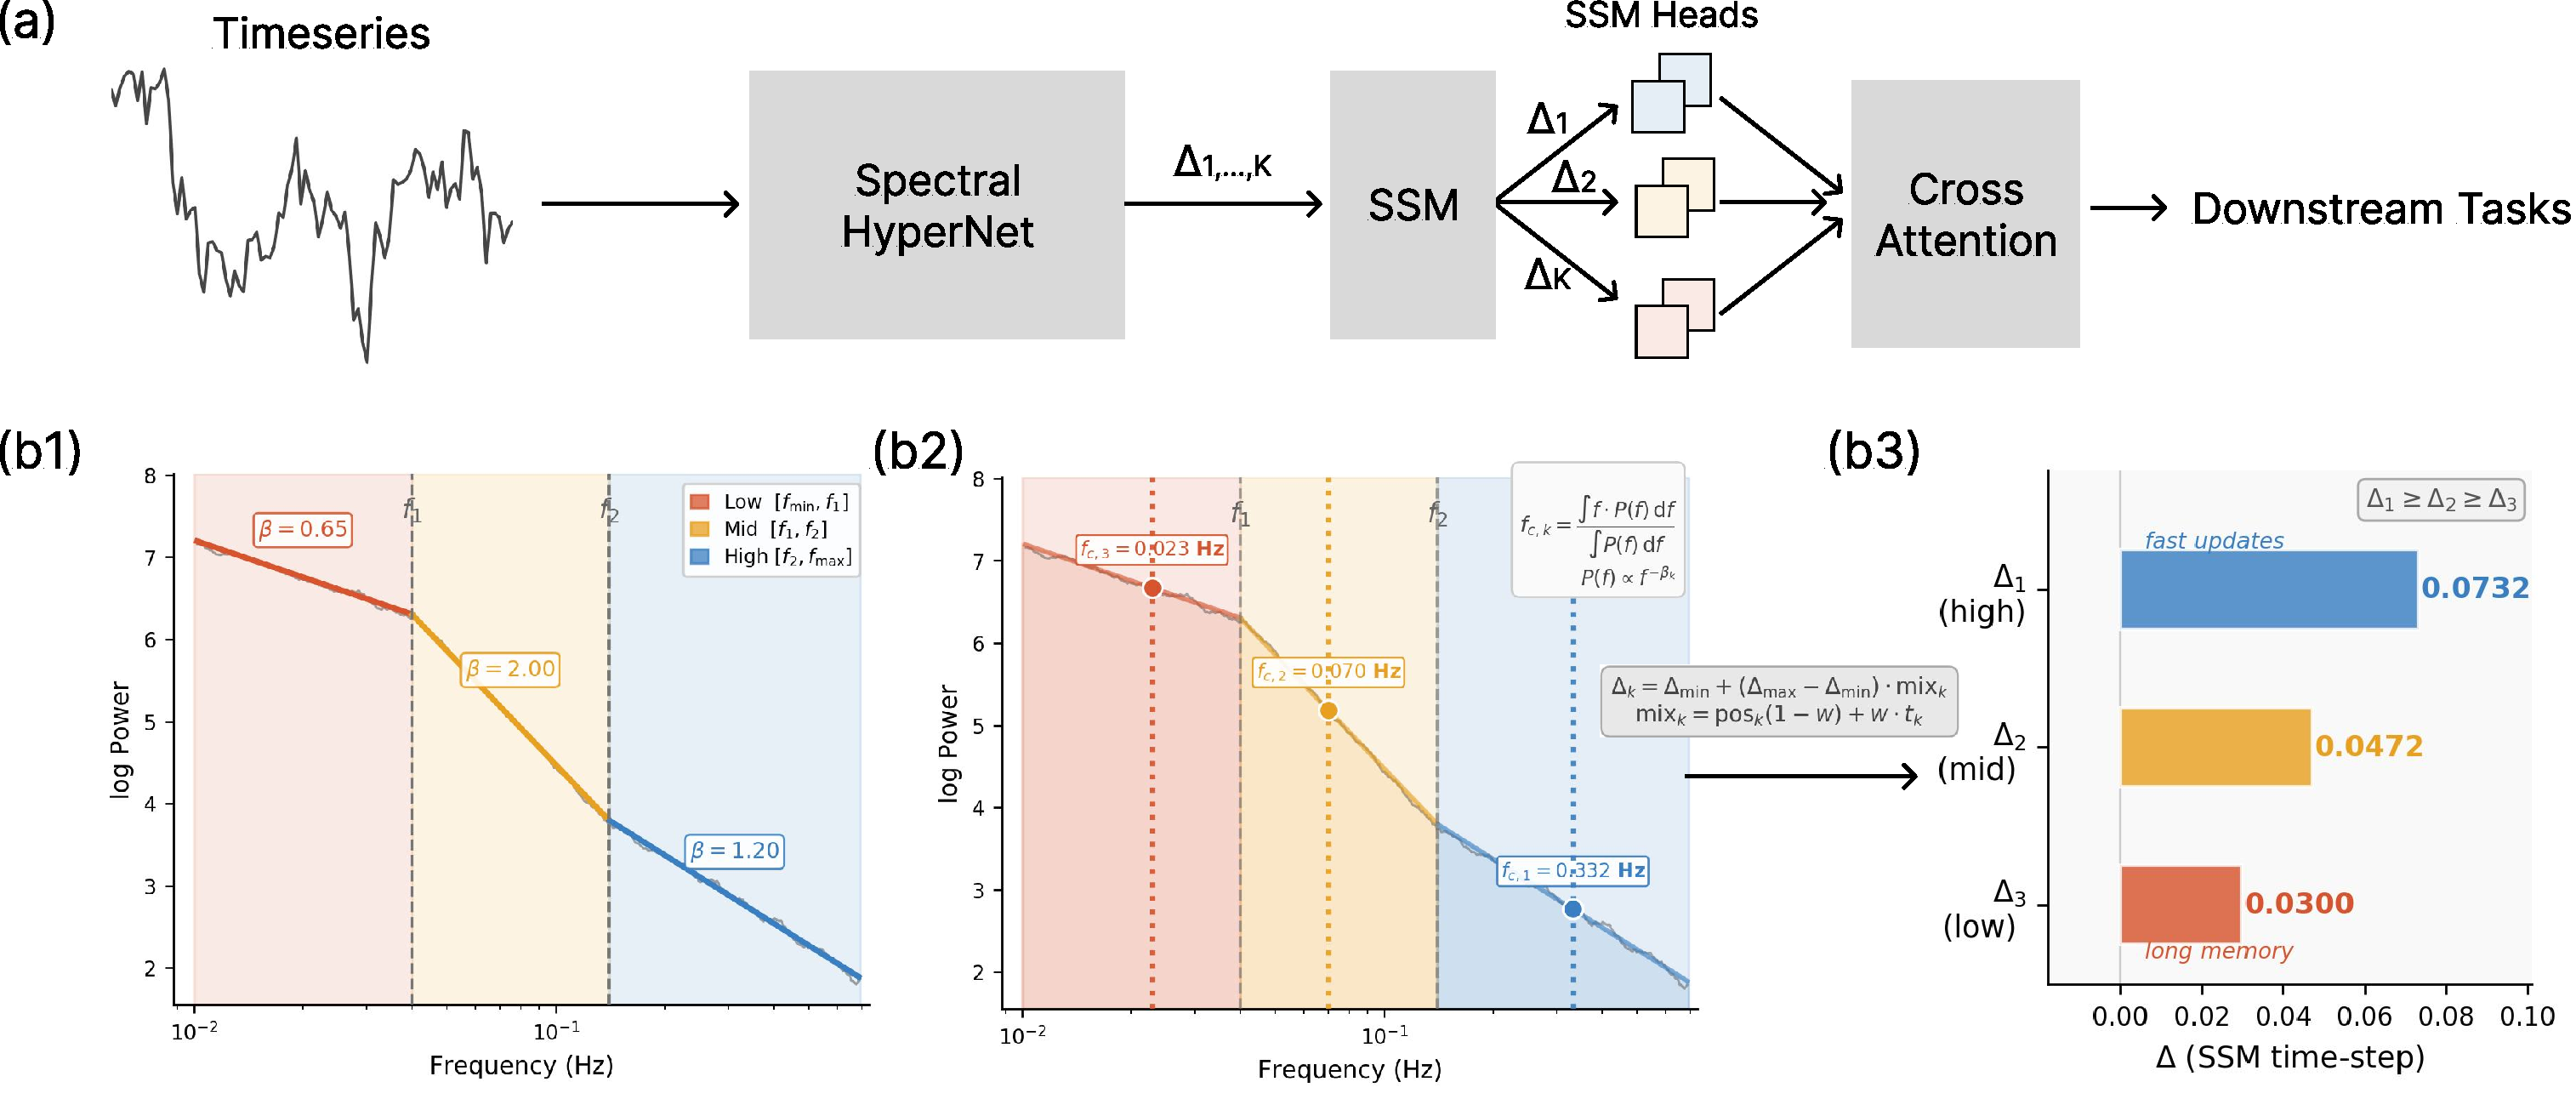
\includegraphics[width=\linewidth]{figures/PIMSM_Fig1.pdf}
\caption{
\textbf{Physics-informed multi-scale parameterization of temporal dynamics.}
\textbf{(a)} SpectralHyperNet computes the input PSD, estimates knee frequencies and spectral exponents, and fits a piecewise power-law PSD.
\textbf{(b1--b3)} The knees partition the frequency axis, not the time series; an energy-weighted representative frequency from each regime is mapped to ordered discretization parameters (shown for the default $K=3$ setting) for fast-to-slow SSM heads, whose states interact through cross-scale attention.
}
\label{fig:architecture_multiscale}
\end{figure}

PIMSM integrates multi-scale temporal structure into a state-space framework without relying on modality-specific components. As shown in Fig.~\ref{fig:architecture_multiscale}, SpectralHyperNet summarizes the input spectrum with knee frequencies and scaling exponents, and these spectral estimates parameterize scale-specific SSM timesteps $\Delta_k$. The original time-domain sequence is then processed by SSM head groups with distinct fast-to-slow temporal kernels, and cross-scale attention models interactions among the resulting scale-specific states before task prediction. The number of knees is configurable through the number of scale groups; the main experiments use the default $K=3$ regime setting as a concrete instance rather than an architectural restriction.

\subsection{Datasets}
\label{sec:methods:data}

Full dataset details and preprocessing are in Appendix~\ref{sec:appx:data}.
\textbf{HCP motor fMRI} (360 cortical ROIs, TR$=0.72$\,s, 5 motor conditions): primary benchmark for temporal-context truncation (backbone input restricted to the first 2/3 TRs of each trial) and low-resource transfer (1--100\% labels).
\textbf{HCP resting-state fMRI}: models trained on rest (284 TRs) and evaluated on motor-task fMRI without adaptation (brain-state shift).
\textbf{Weather-5K}~\citep{han2024far}: 5,672 global weather stations; cross-domain benchmark using hourly multivariate forecasting under a spatial OOD split, where geographically isolated held-out stations are never observed during training. We prioritize this split because held-out stations directly test transfer to unseen geographic domains, whereas chronological holdouts evaluate later windows from already observed stations.

\subsection{SpectralHyperNet: Spectrum-Guided Scale Inference}

We model the power spectral density of each multivariate time series using the piecewise power-law form in Eq.~\eqref{eq:piecewise_powerlaw}, with a configurable number of frequency regimes. The main experiments use the default $K=3$ setting, separated by knee frequencies $(f_1, f_2)$.
We empirically verify this piecewise structure across datasets and domains in Appendix~\ref{sec:appx:psd_multifractal}.

\textbf{Spectral modeling.} Given a spectral context sequence $x^{\mathrm{spec}}$, we estimate the power spectral density $P(f)$ via FFT and fit the piecewise power-law form in Eq.~\eqref{eq:piecewise_powerlaw}. By default, $x^{\mathrm{spec}}$ is the same sequence processed by the SSM backbone; in HCP early-window experiments, SpectralHyperNet instead receives the full trial for spectral calibration while the SSM backbone receives only the first 3 or 2 TRs. This experiment-specific choice tests whether full-sequence spectral structure stabilizes shortened task evidence, and does not simulate a changed scanner TR. In the default $K=3$ setting, $(f_1, f_2)$ denote the two knee frequencies separating three regimes.

\textbf{Knee estimation.} SpectralHyperNet predicts the $K-1$ knee frequencies and $K$ scaling exponents from the spectrum, initialized from a data-driven scipy fit on the first training batch. A multi-resolution MAE spectral fit loss drives knee placement and a seam loss encourages piecewise continuity; hyperparameters are in Appendix~\ref{sec:appx:training_details}.

\textbf{Energy-weighted center frequency and discretization mapping.} The knees define frequency bands, but PIMSM does not use the geometric midpoint of each band as its scale. Instead, for a band $[f_a,f_b]$ with fitted slope $P_k(f)\propto f^{-\beta_k}$, we compute the energy centroid
\[
f_{c,k}=\frac{\int_{f_a}^{f_b} f\,P_k(f)\,df}{\int_{f_a}^{f_b} P_k(f)\,df}.
\]
The implementation evaluates this centroid in closed form, with stable special cases for $\beta_k\approx 1$ and $\beta_k\approx 2$. Thus, a band whose spectral mass is concentrated near its lower boundary yields a lower representative frequency than a midpoint rule would, while flatter bands place the representative frequency closer to the center of the interval.

\paragraph{Frequency-to-delta mapping.}
The core principle is $\Delta_k \propto f_{c,k}$: higher-frequency bands receive larger $\Delta$ (faster updates); lower-frequency bands receive smaller $\Delta$ (longer memory).
We mix global band position $p_k$ and within-band normalized frequency $t_k$ via $m_k = p_k(1-w) + w\,t_k$ ($w=0.3$), yielding $\Delta_k = \Delta_{\min} + (\Delta_{\max} - \Delta_{\min})\cdot m_k$.
A hierarchical constraint $\Delta_1 \ge \Delta_2 \ge \Delta_3$ enforces temporal ordering. Ablations over $w$ and normalization mode are in Appendix~\ref{sec:appx:delta_ablation}.

\begin{table}[t]
\centering
\footnotesize
\begin{tabular}{p{0.96\linewidth}}
\toprule
\textbf{Algorithm 1: Spectrum-to-$\Delta$ parameterization in PIMSM} \\
\midrule
\textbf{Input:} time-domain sequence $x_{1:T}$ for the SSM backbone; spectral context $x^{\mathrm{spec}}$ (the same sequence by default, or a longer full-trial/full-run context in early-window HCP experiments); frequency bounds $[f_{\min}, f_{\max}]$; number of scales $K$ (default $K=3$). \\
\textbf{1. PSD estimation:} compute $P(f)=|\mathrm{FFT}(x^{\mathrm{spec}})|^2$ over non-DC frequencies in $[f_{\min}, f_{\max}]$. \\
\textbf{2. Piecewise spectral fit:} SpectralHyperNet predicts $K-1$ knees and $K$ exponents; a differentiable piecewise power-law $\hat P(f)\propto f^{-\beta_k}$ is fit to $P(f)$ with spectral-fit and seam-continuity losses. \\
\textbf{3. Representative frequencies:} the knees define $K$ frequency bands; for each band, compute $f_{c,k}=\int fP_k(f)df/\int P_k(f)df$ under the fitted exponent $\beta_k$. \\
\textbf{4. Delta mapping:} map each $f_{c,k}$ to a scale-specific timestep $\Delta_k$ using $\Delta_k \propto f_{c,k}$; in the default implementation, $m_k=p_k(1-w)+w\,t_k$ with $w=0.3$ and $\Delta_k=\Delta_{\min}+(\Delta_{\max}-\Delta_{\min})m_k$, followed by an ordered fast-to-slow constraint over $\{\Delta_k\}_{k=1}^{K}$. \\
\textbf{5. Time-domain SSM processing:} process the original sequence $x_{1:T}$ without splitting or filtering it; SSM heads assigned to scale $k$ share $\Delta_k$, and their scale-specific states interact through cross-scale attention before prediction. \\
\bottomrule
\end{tabular}
\caption{Operational summary of the PIMSM spectrum-to-dynamics mapping.}
\label{alg:spectrum_to_delta}
\end{table}

\textbf{Acquisition-unit anchoring.} The SSM transition depends on the product of the discretization step and the continuous-time state matrix (e.g., $\exp(\Delta A)$), so $\Delta$ and $A$ can compensate for one another if both are left unconstrained. PIMSM separates these roles by anchoring them from both sides. First, the spectrum-to-delta map expresses each $\Delta_k$ in dataset-native acquisition units and applies a log-scale regularizer to discourage arbitrary rescaling. Second, the continuous-time decay is initialized as $A=-\exp(A_{\log})$ with $A\approx -1/\tau$ and $\tau$ sampled from a log-uniform acquisition-time range. During training, an $A$-scale penalty
\[
\mathcal{L}_{A}
= \left(\log \overline{|A|} - \log a_0\right)^2,
\qquad
\overline{|A|}=\mathrm{mean}_j\,\exp(A_{\log,j}),
\]
keeps the average decay scale near its initialization $a_0$. This prevents $A$ from simply rescaling to undo the spectrum-derived $\Delta_k$, making the induced effective timescales $\tau_{\mathrm{eff}}\approx \Delta/|A|$ more identifiable in physical time units. Implementation details are in Appendix~\ref{sec:appx:arch_details}.

\subsection{Multi-Scale State-Space Block}

Each PIMSM block extends the Mamba-2 Structured State Space Duality (SSD) kernel~\citep{dao2024transformers} to a multi-scale setting because its multi-head SSM structure provides a natural unit for assigning different discretization parameters to different head groups. This makes Mamba-2 a convenient backbone for multi-scale temporal parameterization: PIMSM can introduce fast-to-slow temporal kernels by sharing $\Delta_k$ within each scale group, without substantially increasing the parameter count relative to a single-scale Mamba2 baseline. Heads within the same scale share $\Delta_k$ but maintain independent state transitions; using multiple heads per scale increases within-scale representational capacity while preserving the intended temporal hierarchy. The resulting scale-specific states are fused through lightweight cross-scale attention to model interactions among temporal scales. Full architectural equations and head counts are given in Appendix~\ref{sec:appx:arch_details}.

\subsection{Backbone, Prediction Head, and Training}
\label{sec:methods:training}

The final hidden sequence is temporally pooled and passed to a task-specific prediction head for classification or forecasting. All models are trained under a shared protocol with matched parameter budgets across baselines. Architecture dimensions and parameter-matching details are provided in Appendix~\ref{sec:appx:arch_details}; optimization settings, Weather-5K preprocessing, RevIN normalization~\citep{kim2021reversible}, and OOD split construction are reported in Appendix~\ref{sec:appx:training_details} and Appendix~\ref{sec:appx:data}.


\section{Results}\label{sec:results}

We evaluate PIMSM across four deployment-motivated axes of structured distribution shift. Axes (i--ii) use HCP motor fMRI; axis (iii) uses HCP resting-state$\to$task fMRI; axis (iv) uses Weather-5K spatial OOD forecasting. All comparisons use parameter-matched baselines (Mamba2, Transformer, 1D-CNN), with $\approx$7.85M parameters for HCP experiments and $\approx$18M parameters for Weather-5K forecasting.

\subsection{Axis (i): Temporal-Context Shift --- HCP Motor Early-Window Truncation}
\label{sec:results:hcp_tr_shift}

\begin{figure}[htbp]
\centering
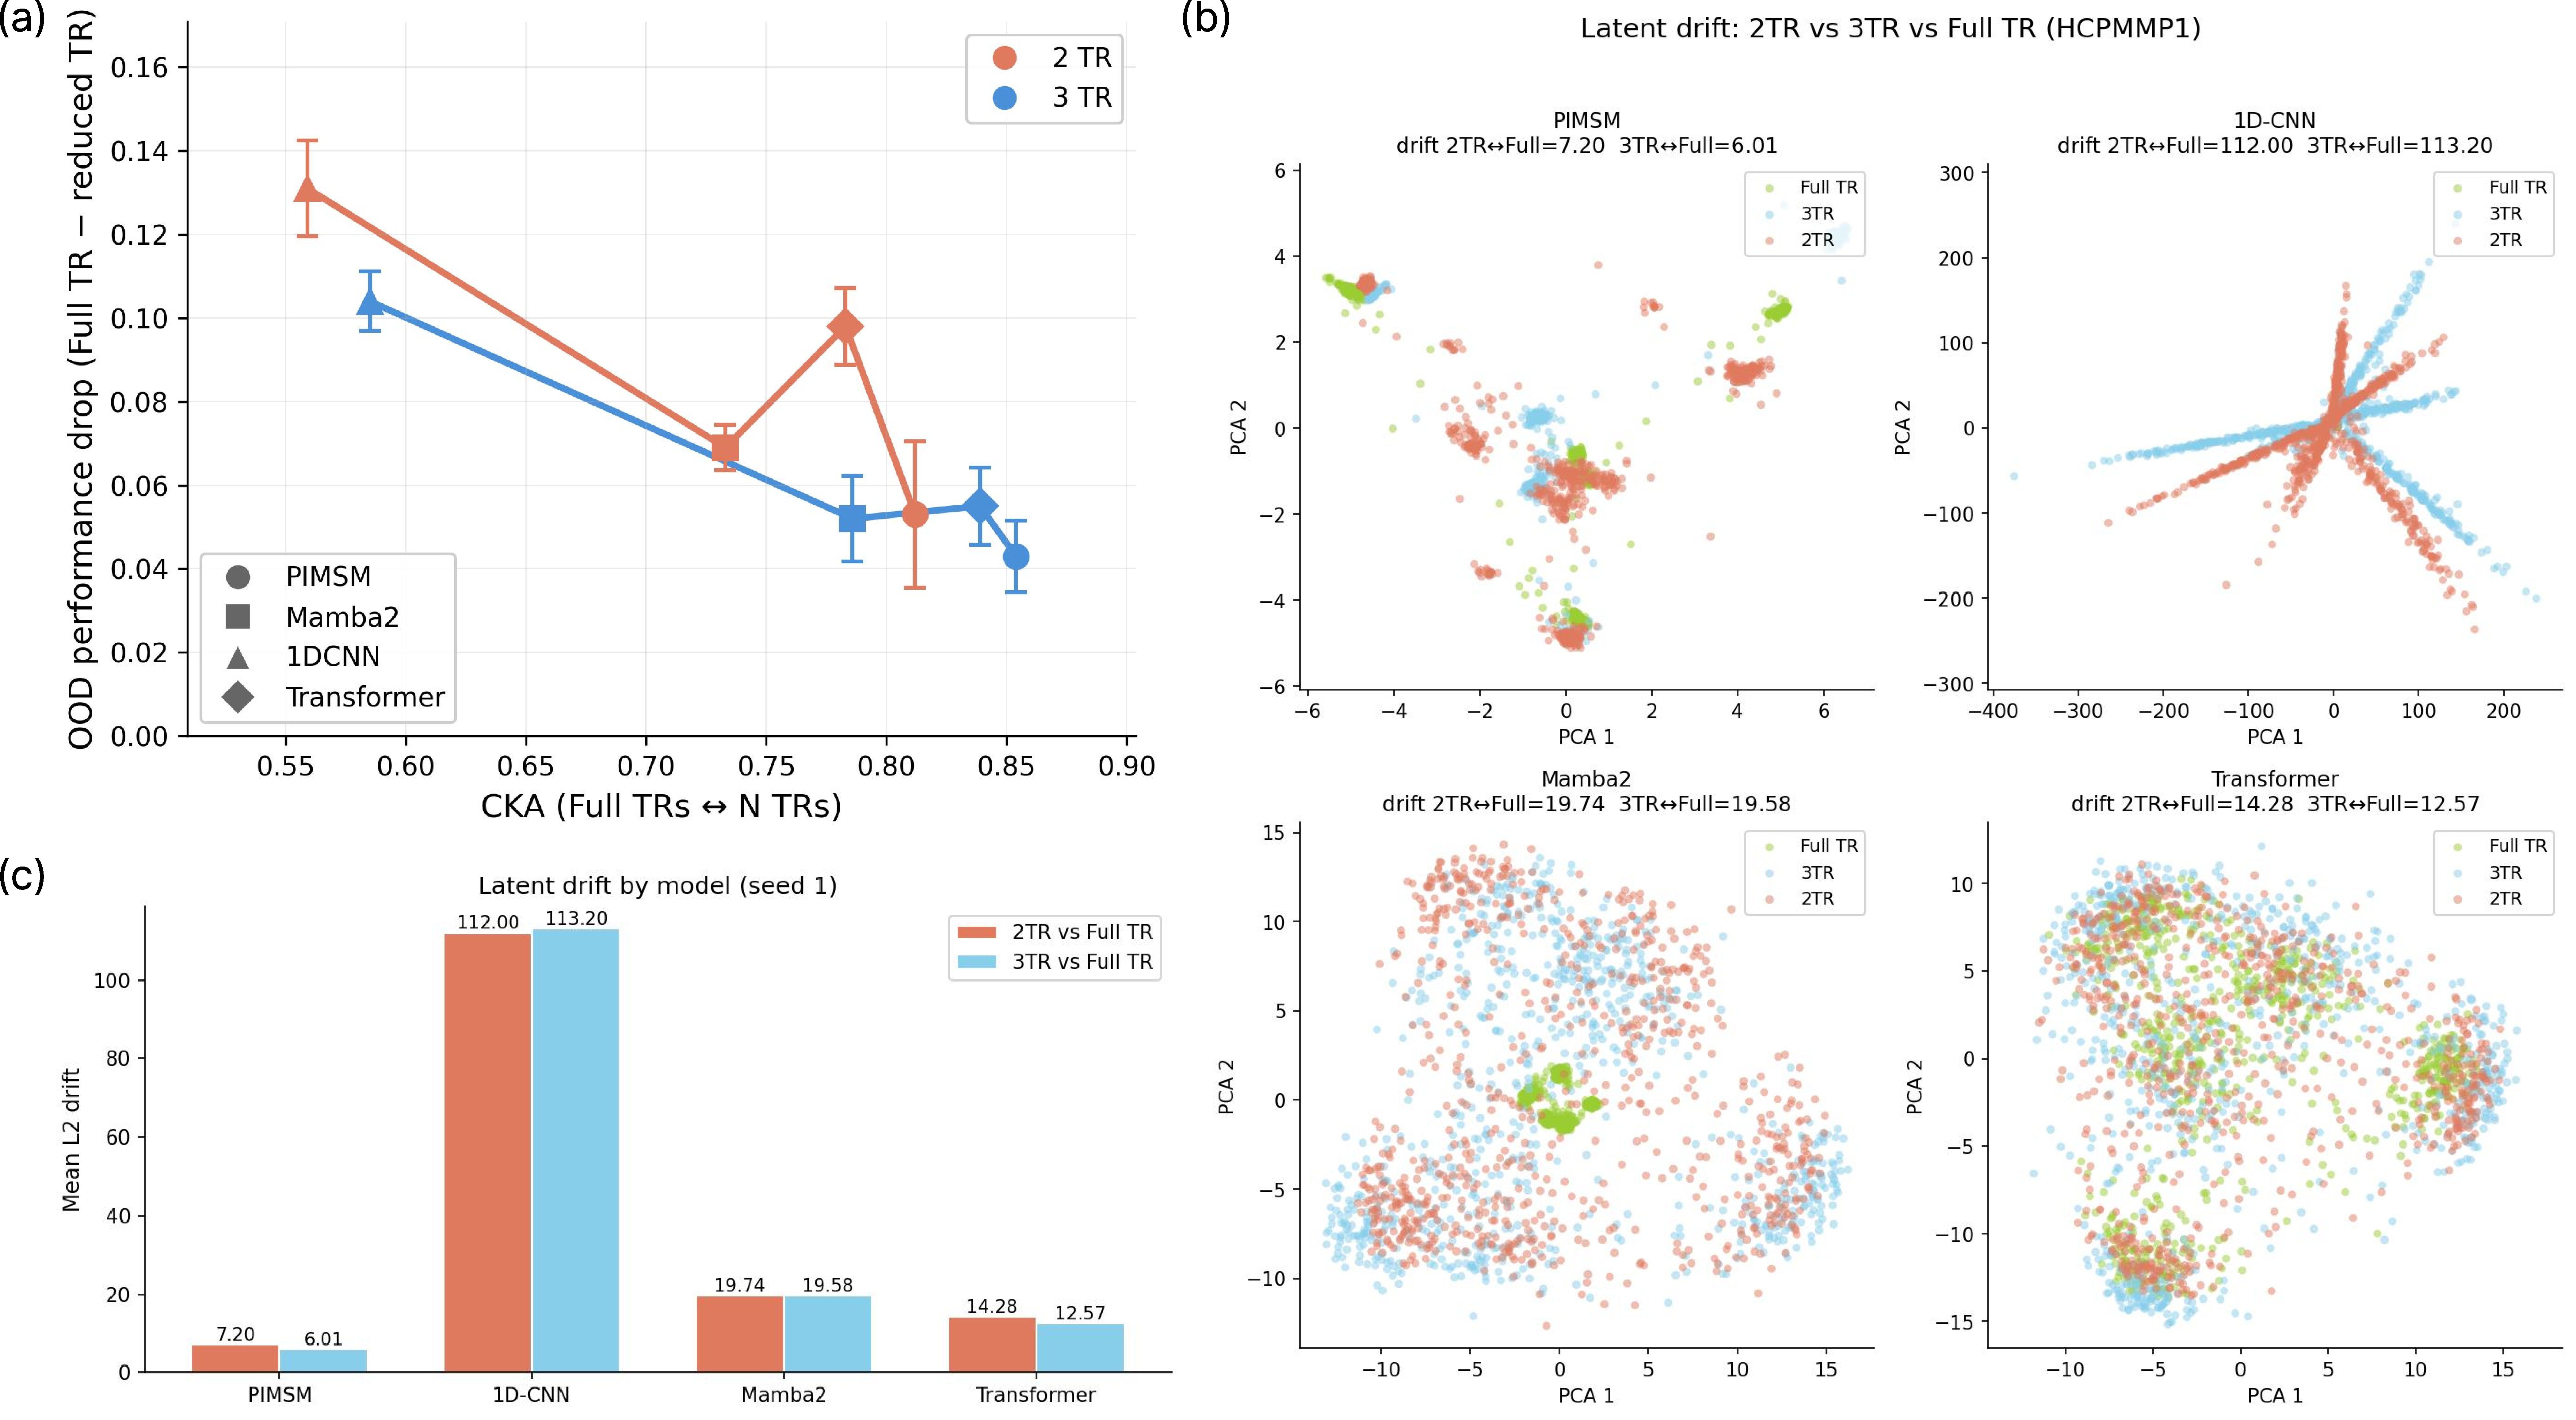
\includegraphics[width=\linewidth]{figures/PIMSM_Fig2.pdf}
\caption{
\textbf{Representation stability under temporal-context truncation (HCP motor task fMRI).}
\textbf{(a)} Relationship between representation similarity (CKA; full trial vs early-window inputs) and performance drop (full trial $\rightarrow$ 2TR / 3TR).
\textbf{(b)} PCA visualization of latent embeddings under full-trial, 3TR, and 2TR inputs.
\textbf{(c)} Mean $\ell_2$ latent drift between full-trial and early-window conditions.
}
\label{fig:tr_shift_stability}
\end{figure}

We assess robustness to temporal-context shift by truncating the SSM backbone input for each motor trial to the first 3 or 2 TRs, simulating severe early-window decoding while preserving task labels and subject identity.
SpectralHyperNet still receives the full trial sequence to estimate the spectral hierarchy used for scale calibration; therefore this experiment isolates whether full-sequence spectral structure can stabilize representations when downstream task evidence is temporally shortened, rather than simulating a changed scanner TR.
Figure~\ref{fig:tr_shift_stability} reports representation stability (CKA, distance correlation dCor between full-trial and truncated-input representations) alongside decoding accuracy.

\paragraph{Full trial $\rightarrow$ 2 TRs (severe truncation).}
Table~\ref{tab:drift2tr} shows that PIMSM has the smallest full-trial$\to$2TR accuracy drop while also achieving the highest representation similarity between full-trial and truncated-input embeddings, measured by both CKA and dCor.
This pattern is more informative than shifted accuracy alone: PIMSM preserves the latent geometry of the full-trial solution when only the earliest time points are available.
Replacing spectrum-derived $\Delta$ with learnable or random values increases the accuracy drop and lowers CKA/dCor, indicating that robustness is not explained by multi-scale capacity alone but by spectrum-aligned temporal anchoring.
Representation stability metrics provide a cleaner signal than accuracy alone for isolating this contribution: PIMSM~(learnable~$\Delta$) reaches a 2TR accuracy similar to Mamba2 ($0.913\pm0.030$ vs.\ $0.914\pm0.005$), yet its representation geometry under truncation is markedly weaker than full PIMSM---CKA increases from $0.776\pm0.086$ to $0.812\pm0.033$, with the reduced cross-seed variance indicating that spectrum-derived initialization anchors the representation geometry more consistently across runs.
Across the three paired seeds, PIMSM improves over Mamba2 on all shifted 2TR metrics (accuracy, accuracy drop, CKA, and dCor).
Given the small seed count, we treat paired tests as exploratory rather than definitive; the consistent direction of CKA and dCor improvements across all three seeds supports the robustness of the representation-stability effect.

\begin{table}[htbp]
\centering
\footnotesize
\begin{tabular}{lcccc}
\toprule
Model & Full trial & 2 TRs & CKA (Full trial$\leftrightarrow$2TR) & dCor (Full trial$\leftrightarrow$2TR) \\
\midrule
Mamba2 & $0.983\pm0.002$ & $0.914\pm0.005$ & $0.733\pm0.018$ & $0.770\pm0.011$ \\
1DCNN & $0.978\pm0.007$ & $0.847\pm0.009$ & $0.559\pm0.020$ & $0.622\pm0.012$ \\
Transformer & $0.982\pm0.006$ & $0.884\pm0.007$ & $0.783\pm0.015$ & $0.805\pm0.005$ \\
PIMSM (learnable $\Delta$) & $0.982\pm0.001$ & $0.913\pm0.030$ & $0.776\pm0.086$ & $0.804\pm0.078$ \\
PIMSM (random $\Delta$) & $0.983\pm0.004$ & $0.889\pm0.055$ & $0.737\pm0.105$ & $0.774\pm0.108$ \\
\midrule
\textbf{PIMSM} & $\mathbf{0.987\pm0.007}$ & $\mathbf{0.933\pm0.016}$ & $\mathbf{0.812\pm0.033}$ & $\mathbf{0.846\pm0.022}$ \\
\bottomrule
\end{tabular}
\caption{
\textbf{HCP motor decoding under severe temporal-context truncation (full trial $\rightarrow$ 2 TRs).}
Values are mean $\pm$ std over three seeds. PIMSM achieves the highest accuracy and representation stability. Representation stability (CKA, dCor) is the primary discriminator between initialization strategies: PIMSM~(learnable~$\Delta$) matches Mamba2 in 2TR accuracy yet achieves lower CKA ($0.776$ vs.\ $0.812$) with higher cross-seed variance, confirming that spectrum-derived initialization---not multi-scale capacity alone---is responsible for the geometry-preservation benefit.
}
\label{tab:drift2tr}
\end{table}

\paragraph{Full trial $\rightarrow$ 3 TRs (moderate truncation).}
Under the milder full-trial $\rightarrow$ 3 TRs setting, PIMSM shows the same trend, achieving the best 3TR accuracy and stable representations among parameter-matched baselines (Appendix Table~\ref{tab:drift3tr}).
The same paired-seed pattern holds at 3TR: PIMSM improves over Mamba2 on accuracy, CKA, and dCor for all three seeds, again supporting the robustness trend without claiming formal statistical significance.

\paragraph{Drift intervention and scaling.}
Explicit drift regularization on Mamba2 improves stability without degrading ID performance, providing evidence that representation drift is a useful intervention target; PIMSM achieves comparable stability through architecture alone (detailed tables and scaling figures in Appendix~\ref{sec:appx:hcp_tr_shift}).

\subsection{Axis (ii): Low-Resource Generalization — HCP Motor Data Scarcity}
\label{sec:results:data_scarce}

Table~\ref{tab:data_scarce} reports motor decoding accuracy as labeled training data varies from 1\% to 100\%.
The data-scarce split is implemented by first constructing the standard subject-level train/validation/test split and then randomly subsampling only the training set according to the specified data ratio; validation and test subjects are kept fixed.
Thus, the 1\% condition evaluates whether a model trained from an extremely small labeled training subset still generalizes to the same held-out motor-task test distribution, rather than making the test set smaller or easier.
In this most data-scarce setting, PIMSM is the strongest model, indicating that spectrum-aligned temporal kernels are most useful when the supervised signal is extremely limited.
As the label budget increases, differences among architectures narrow and the advantage is no longer uniform, suggesting that the main benefit is improved sample efficiency under extreme supervision scarcity rather than blanket dominance across all data regimes.
Pretraining on resting-state fMRI further improves robustness; linear probing results are reported in Appendix~\ref{sec:appx:pretrain}.

\begin{table}[htbp]
\centering
\footnotesize
\begin{tabular}{lcccc}
\toprule
Model & 1\% & 5\% & 10\% & 100\% \\
\midrule
PIMSM & $\mathbf{0.797\pm0.040}$ & $0.940\pm0.017$ & $0.963\pm0.011$ & $\mathbf{0.987\pm0.007}$ \\
Mamba2 & $0.752\pm0.015$ & $0.934\pm0.022$ & $0.963\pm0.006$ & $0.983\pm0.002$ \\
1DCNN & $0.709\pm0.026$ & $0.927\pm0.018$ & $0.956\pm0.007$ & $0.978\pm0.007$ \\
Transformer & $0.774\pm0.031$ & $\mathbf{0.948\pm0.017}$ & $\mathbf{0.967\pm0.006}$ & $0.982\pm0.006$ \\
\bottomrule
\end{tabular}
\caption{
\textbf{Low-resource generalization on HCP motor decoding.}
Values are mean $\pm$ std over three seeds. Models are pretrained on resting-state fMRI and finetuned with varying fractions of labeled data.
PIMSM performs best in the extreme low-data regime (1\%).
}
\label{tab:data_scarce}
\end{table}

\subsection{Axis (iii): Brain-State Shift --- Resting-State → Task Generalization}
\label{sec:results:brainstateshift}

We train on HCP resting-state fMRI for sex classification and evaluate the same task label on motor-task fMRI without adaptation, testing whether temporal kernels learned from spontaneous dynamics remain useful under task-evoked acquisition state.
We use sex classification because the label is defined independently of scan condition and is available for both resting-state and task-fMRI, allowing the evaluation to change brain/acquisition state while keeping the prediction target fixed.
We do not report CKA/dCor for Axis (iii) because resting-state and task-fMRI are not paired observations of the same input under two temporal conditions; cross-condition similarity would conflate representation stability with differences in behavioral state and sequence content.
PIMSM achieves the highest accuracy and substantially lower cross-seed variance (Table~\ref{tab:brainstateshift}), suggesting reduced sensitivity to resting$\leftrightarrow$task reconfiguration in this setting rather than only a higher mean score.

\begin{table}[htbp]
\centering
\footnotesize
\begin{tabular}{lc}
\toprule
Model & Accuracy \\
\midrule
Mamba2      & $0.591\pm0.038$ \\
1D-CNN      & $0.589\pm0.040$ \\
Transformer & $0.554\pm0.063$ \\
\midrule
\textbf{PIMSM} & $\mathbf{0.632\pm0.013}$ \\
\bottomrule
\end{tabular}
\caption{
\textbf{Brain-state shift: resting-state training $\to$ motor-task test (Axis iii).}
Values are mean $\pm$ std over three seeds. Models are trained for sex classification on HCP resting-state fMRI and evaluated on HCP motor-task fMRI without adaptation; the target label is shared across both scan conditions.
PIMSM achieves the highest accuracy and the lowest cross-seed variance among the baselines in this setting, consistent with the hypothesis that physics-informed multi-scale kernels reduce sensitivity to resting$\to$task reconfiguration.
}
\label{tab:brainstateshift}
\end{table}

\subsection{Axis (iv): Cross-Domain Shift — Weather-5K}
\label{sec:results:weather}

We evaluate whether the same spectrum-guided temporal parameterization transfers to meteorological forecasting without domain-specific adaptation.
Weather-5K is a substantially different modality and sampling regime from fMRI, with hourly station measurements and heterogeneous target units; Table~\ref{tab:weather} therefore reports variable-wise MAE under the held-out-station spatial OOD split.
Across forecasting horizons, PIMSM attains the lowest MAE on all 24 variable-horizon endpoints, including scalar meteorological variables (TMP, SLP, DEW), wind rate, and both wind-angle components.
Against the best non-PIMSM baseline for each endpoint, PIMSM reduces MAE by 15.2\% on average, with larger gains at longer horizons (11.4\% at 24h versus 17.9\% at 168h).
\begin{table}[htbp]
\centering
\scriptsize
\setlength{\tabcolsep}{1.1pt}
\begin{tabular}{llcccccc}
\toprule
Horizon & Model & TMP & SLP & DEW & Wind Rate & Wind Cos & Wind Sin \\
\midrule
24h & Mamba2      & $1.823\pm0.127$ & $2.486\pm0.379$ & $1.951\pm0.287$ & $1.903\pm0.009$ & $0.561\pm0.000$ & $0.530\pm0.020$ \\
    & 1D-CNN      & $1.150\pm0.066$ & $1.505\pm0.462$ & $1.316\pm0.213$ & $1.330\pm0.008$ & $0.416\pm0.000$ & $0.389\pm0.018$ \\
    & Transformer & $1.351\pm0.078$ & $2.066\pm0.648$ & $1.417\pm0.256$ & $1.537\pm0.009$ & $0.462\pm0.000$ & $0.450\pm0.018$ \\
    & \textbf{PIMSM} & $\mathbf{0.921\pm0.052}$ & $\mathbf{1.190\pm0.341}$ & $\mathbf{1.066\pm0.041}$ & $\mathbf{1.301\pm0.154}$ & $\mathbf{0.410\pm0.005}$ & $\mathbf{0.370\pm0.014}$ \\
\midrule
72h & Mamba2      & $1.827\pm0.533$ & $3.984\pm0.640$ & $2.513\pm0.121$ & $1.949\pm0.312$ & $0.587\pm0.011$ & $0.591\pm0.007$ \\
    & 1D-CNN      & $1.541\pm0.247$ & $2.931\pm0.776$ & $1.855\pm0.613$ & $1.569\pm0.353$ & $0.479\pm0.019$ & $0.482\pm0.077$ \\
    & Transformer & $2.266\pm0.678$ & $3.911\pm0.946$ & $2.017\pm0.163$ & $1.732\pm0.351$ & $0.533\pm0.012$ & $0.513\pm0.024$ \\
    & \textbf{PIMSM} & $\mathbf{1.167\pm0.127}$ & $\mathbf{2.214\pm0.826}$ & $\mathbf{1.411\pm0.108}$ & $\mathbf{1.512\pm0.204}$ & $\mathbf{0.475\pm0.013}$ & $\mathbf{0.439\pm0.018}$ \\
\midrule
120h & Mamba2      & $2.469\pm0.287$ & $4.522\pm0.778$ & $2.797\pm0.235$ & $2.010\pm0.468$ & $0.594\pm0.013$ & $0.624\pm0.033$ \\
     & 1D-CNN      & $1.790\pm0.184$ & $3.390\pm1.359$ & $2.222\pm0.247$ & $1.633\pm0.324$ & $0.508\pm0.018$ & $0.527\pm0.039$ \\
     & Transformer & $2.108\pm0.321$ & $4.629\pm1.278$ & $2.312\pm0.165$ & $1.818\pm0.315$ & $0.551\pm0.017$ & $0.580\pm0.045$ \\
     & \textbf{PIMSM} & $\mathbf{1.263\pm0.153}$ & $\mathbf{2.585\pm0.991}$ & $\mathbf{1.546\pm0.131}$ & $\mathbf{1.565\pm0.214}$ & $\mathbf{0.494\pm0.012}$ & $\mathbf{0.457\pm0.021}$ \\
\midrule
168h & Mamba2      & $2.588\pm0.290$ & $4.848\pm0.863$ & $2.922\pm0.215$ & $2.021\pm0.336$ & $0.596\pm0.010$ & $0.627\pm0.009$ \\
     & 1D-CNN      & $2.009\pm0.301$ & $3.748\pm1.012$ & $2.516\pm0.299$ & $1.667\pm0.346$ & $0.523\pm0.008$ & $0.556\pm0.015$ \\
     & Transformer & $2.159\pm0.341$ & $4.724\pm1.126$ & $2.294\pm0.198$ & $1.747\pm0.312$ & $0.537\pm0.011$ & $0.580\pm0.025$ \\
     & \textbf{PIMSM} & $\mathbf{1.334\pm0.167}$ & $\mathbf{2.849\pm1.069}$ & $\mathbf{1.638\pm0.139}$ & $\mathbf{1.610\pm0.215}$ & $\mathbf{0.506\pm0.012}$ & $\mathbf{0.476\pm0.019}$ \\
\bottomrule
\end{tabular}
\caption{
\textbf{Weather-5K cross-domain forecasting (Axis iv).}
Values are mean $\pm$ std. Variable-wise spatial OOD MAE is reported for temperature (TMP), sea-level pressure (SLP), dew point (DEW), wind rate, and wind angle components (cos/sin) across 24h, 72h, 120h, and 168h forecasting horizons. PIMSM is applied without domain-specific adaptation.
}
\label{tab:weather}
\end{table}


\section{Related Work}
\label{sec:related}

\paragraph{Foundation models for scientific time series.}
Brain foundation models and time-series forecasting foundation models demonstrate the value of large-scale pretraining, zero-/low-shot adaptation, and reusable representations across datasets~\citep{tak2026generalizable,wang2025towards,wang2025slim,wang2026omni,abhimanyu2024decoder,ansari2024chronos,woo2024unified}.
These works primarily ask how far representation learning can be pushed by larger corpora, generic sequence objectives, or adaptation modules.
PIMSM is complementary: it asks whether the backbone itself preserves physically meaningful temporal scales under shift, even without modality-specific components or shift-specific supervision.

\paragraph{Multi-scale state-space and Mamba models.}
Recent multi-scale SSM/Mamba variants motivate the need for temporal hierarchy, but instantiate scale in different ways.
MS-SSM~\citep{Karami2025MSSSMAM} processes multiple resolutions with specialized state-space dynamics and an input-dependent scale mixer.
ms-Mamba~\citep{karadag2025ms} uses multiple Mamba blocks with different sampling rates to model forecasting signals at several temporal scales.
STM3~\citep{chen2025stm3} targets long-term spatio-temporal prediction with multiscale Mamba experts, adaptive graph causal convolution, and mixture-of-experts routing.
WMF-Traffic~\citep{li2025multi} combines wavelet decomposition, traffic-aware Mamba, and Fourier adjustment for traffic forecasting.
PIMSM differs from these scale-by-design approaches by deriving scale-specific discretization from empirical spectra, enforcing an ordered temporal hierarchy through knee frequencies and energy-weighted representative frequencies, and anchoring both $\Delta$ and $A$ in dataset-native acquisition units.

\section{Discussion}
\label{sec:discussion}

PIMSM supports the view that temporal-scale alignment is a practical inductive bias for scientific sequence models, not merely an architectural detail. Coupling spectrum-derived knee frequencies to scale-specific $\Delta$ values, while anchoring both $\Delta$ and $A$ in acquisition time units, gives the backbone a memory policy tied to the signal's physical organization.

In neural data, this matters most in regimes where ordinary supervision is weak or observation is constrained. Early-window decoding is relevant to low-latency brain-computer interfaces and closed-loop neurotechnology, where decisions must often be made from the earliest available neural evidence. The data-scarce and resting-state$\rightarrow$task experiments address a related deployment reality: task-fMRI labels are expensive and heterogeneous, while resting-state scans are more broadly available.

Weather-5K shows that the same mechanism is not tied to neuroimaging-specific assumptions. Under held-out-station spatial OOD, the larger gains at longer horizons suggest that robust forecasting increasingly depends on preserving longer-range temporal structure rather than fitting short-horizon local patterns alone. This supports the interpretation of PIMSM as a modality-agnostic spectrum-to-memory mechanism.

Several limitations remain. The current HCP temporal-context experiments test input truncation rather than a scanner-level change in TR: SpectralHyperNet receives the full sequence for scale calibration while the SSM backbone receives shortened early-window input. PIMSM also assumes that a small number of spectrum-derived knees usefully summarizes temporal organization; domains without clear piecewise spectral structure, or tasks requiring a different number of scales than the default $K=3$ used here, may require different parameterizations. Acquisition-unit anchoring requires a known sampling interval, and SpectralHyperNet adds FFT and spectral-fit overhead relative to plain Mamba2; full GPU-hour accounting remains future work. Finally, HCP tables report three-seed means and standard deviations rather than formal paired significance tests, contemporaneous multi-scale SSM/Mamba methods are not included as parameter-matched HCP baselines, and Weather-5K is evaluated under held-out-station spatial OOD.


\newpage
\appendix

\section{Training Details}
\label{sec:appx:training_details}

For HCP experiments, all models are trained for 35 epochs using AdamW ($\mathrm{lr} = 10^{-3}$, weight decay $= 0.1$) with cosine annealing and linear warmup. Gradient norms are clipped to 1.0. Label smoothing ($\epsilon = 0.1$) is applied for classification. Batch size is 16 for the brain-state shift experiment (Axis iii) and 32 for motor decoding (Axes i--ii). HCP runs use three random seeds; we report mean $\pm$ standard deviation of test accuracy.

Weather-5K forecasting uses the same parameter-matched backbone family but a forecasting-specific optimization setup: 30 epochs, AdamW with learning rate $5\times10^{-5}$, weight decay $0.05$, cosine scheduling with 5 warmup epochs, batch size 2048, and early stopping on validation MSE. The input window is 48 hourly observations and the prediction head outputs $H\times6$ values for horizons $H\in\{24,72,120,168\}$ hours. Training uses MSE in the globally normalized target space; reported MAE is converted back to original variable units for interpretability.

\textbf{Weather-5K RevIN.}
For Weather-5K, we apply a stateless reversible instance normalization (RevIN)~\citep{kim2021reversible} to reduce station-level mean/variance shortcuts under held-out-station spatial OOD. After the dataset-level training-statistic z-score normalization, RevIN computes the per-window, per-variable mean and standard deviation over time, feeds $(x-\mu)/\sigma$ to the sequence backbone, and denormalizes the $H$-step forecast with the same $(\mu,\sigma)$ before the MSE loss and evaluation metrics are computed. SpectralHyperNet receives the pre-RevIN signal (or an explicit longer spectral context when provided), so PSD-based knee estimation is not driven by the window-wise amplitude removal introduced by RevIN.

The total training objective for PIMSM is:
\begin{equation}
\mathcal{L} = \mathcal{L}_{\mathrm{task}} + w_{\mathrm{fit}}\,\mathcal{L}_{\mathrm{fit}} + w_{\mathrm{seam}}\,\mathcal{L}_{\mathrm{seam}} + \lambda_\Delta\,\mathcal{L}_{\Delta} + \lambda_A\,\mathcal{L}_A + w_{\mathrm{hyp}}\,\mathcal{L}_{\mathrm{hyp}} + \lambda_\beta\,\mathcal{L}_{\beta},
\end{equation}
where:
\begin{itemize}
    \item $\mathcal{L}_{\mathrm{task}}$: cross-entropy classification loss (with label smoothing $\epsilon=0.1$);
    \item $\mathcal{L}_{\mathrm{fit}}$: multi-scale MAE spectral fit loss ($w_{\mathrm{fit}} = 3.0$), averaged equally across all ROIs;
    \item $\mathcal{L}_{\mathrm{seam}}$: piecewise continuity (seam) loss penalizing log-PSD discontinuities at $f_1, f_2$ ($w_{\mathrm{seam}} = 0.1$);
    \item $\mathcal{L}_{\Delta} = \lambda_\Delta\,\mathbb{E}[\log(\Delta/\mathrm{TR})^2]$: TR-anchoring regularization ($\lambda_\Delta = 0.1$);
    \item $\mathcal{L}_A = \lambda_A \sum_j (\log|\bar{A}_j| - \log a_0)^2$: $A$-scale regularization ($\lambda_A = 0.1$);
    \item $\mathcal{L}_{\mathrm{hyp}}$: auxiliary spectral alignment loss ($w_{\mathrm{hyp}} = 0.3$);
    \item $\mathcal{L}_{\beta}$: extreme-$\beta$ regularization penalizing exponents approaching $[0.3, 5.0]$ boundaries ($\lambda_{\beta} = 0.5$).
\end{itemize}
The joint anchoring of $\Delta$, $\tau$-initialization of $A$, and $\mathcal{L}_A$ constitute the default PIMSM protocol across all experiments unless an ablation removes a component.

\section{Architecture Details}
\label{sec:appx:arch_details}

\subsection{Multi-Scale State-Space Block}

Each PIMSM block extends the Mamba-2 Structured State Space Duality (SSD) kernel to a multi-scale setting.

\textbf{Backbone and prediction head.} The backbone consists of nine stacked PIMSM blocks with intermediate gated MLP layers. The model dimension is $d_{\mathrm{model}} = 320$ with an intermediate MLP dimension of $d_{\mathrm{inter}} = 1024$. Temporal mean pooling is applied to the final hidden sequence, followed by a task-specific linear classifier (binary for HCP sex/brain-state shift, 5-class for motor decoding, regression/forecasting for Weather-5K). Parameter counts are matched across all baselines ($\approx$7.85M parameters): Mamba2 ($d_{\mathrm{model}}=352$, 9 layers), Transformer ($d_{\mathrm{model}}=280$, 8 layers), and 1D-CNN (channels 220/440/660/880).

\textbf{Head grouping.} We employ $H = 6$ SSM heads grouped into $K = 3$ scale groups, with two heads per scale. Heads within the same scale share the discretization parameter $\Delta_k$ but maintain independent state transition matrices.

\textbf{State transition initialization.} The SSM $A$ matrix is initialized as $A = -1/\tau$ with $\tau \sim \mathrm{LogUniform}(1 \times \mathrm{TR}, 100 \times \mathrm{TR})$, reflecting the physiologically motivated time-constant range of BOLD dynamics. An $A$-scale regularization $\mathcal{L}_A$ is applied to prevent $A$ from drifting away from this initialization to compensate for $\Delta$, ensuring that the joint constraint on $\tau_\text{eff}$ remains effective throughout training.

\textbf{State evolution.} For each head $j$ assigned to scale $k(j)$, the discretized state update is:
\begin{equation}
\mathbf{h}^{(j)}_t = \bar{A}^{(j)}(\Delta_{k(j)}) \mathbf{h}^{(j)}_{t-1} + \bar{B}(\Delta_{k(j)}) \mathbf{x}_t.
\end{equation}
Input projections are shared across heads, while state transitions differ to capture scale-specific decay dynamics.

\textbf{Scale aggregation.} Within each scale group, head outputs are averaged:
\begin{equation}
\mathbf{h}^{(k)}_t = \frac{1}{|J_k|} \sum_{j \in J_k} \mathbf{h}^{(j)}_t.
\end{equation}

\subsection{Cross-Scale Fusion}

Scale-specific representations are concatenated and passed through a lightweight cross-scale attention module:
\begin{align}
\mathbf{h}_t &= \mathrm{Concat}(\mathbf{h}^{(1)}_t, \mathbf{h}^{(2)}_t, \mathbf{h}^{(3)}_t), \\
\mathrm{Attn}(Q, K, V) &= \mathrm{softmax}\!\left( \frac{QK^\top}{\sqrt{d}} \right) V.
\end{align}
This allows high- and low-frequency information to be selectively combined while preserving structured multi-scale dynamics.

\section{Self-Supervised Pretraining Details}
\label{sec:appx:pretraining}

\paragraph{Uniform spatiotemporal masking.}
We adopt a uniform masking strategy applied jointly over the temporal and spatial dimensions of the input sequence.
Each $(t,r)$ location (time $t$, ROI $r$) is masked independently with a fixed probability of $10\%$.
To further increase reconstruction difficulty and encourage learning of spatial dependencies, we additionally apply ROI-level temporal masking: for each ROI, contiguous time points corresponding to approximately $30\%$ of the sequence length are randomly selected and masked.

\paragraph{SpectralHyperNet during pretraining.}
SpectralHyperNet operates on the \emph{original unmasked} input $x_{1:T}$ to estimate the piecewise power-law parameters:
\[
(f_1, f_2, \beta_1, \beta_2, \beta_3) = H_{\phi}(x_{1:T}).
\]
Importantly, the knee frequencies $(f_1, f_2)$ determine the scale-specific discretization parameters $\Delta_k$ (via the energy-weighted center frequency mapping $\Delta_k = \Psi(f_{c,k})$), while the scaling exponents $\beta_k$ serve as supervision targets for the spectral fit loss and inform the energy-weighted computation of $f_{c,k}$; they do not appear explicitly in the $\Delta_k$ formula. This design ensures that spectral estimates remain stable even when the input to the SSM backbone is partially corrupted by masking.

\paragraph{Training objective.}
The reconstruction loss is an $L_1$ loss over masked positions only:
\[
\mathcal{L}_{\text{pretrain}} = \| x_{\text{masked}} - \hat{x}_{\text{masked}} \|_1.
\]

% -----------------------------------------------------------------------
% ABCD TR downsampling section — commented out (harmonized data; site effect removed)
% -----------------------------------------------------------------------
% \section{ABCD Resting-State: Temporal-Resolution Robustness and Site CKA}
% \label{sec:appx:abcd_tr}
%
% \paragraph{Temporal-resolution (TR downsampling).}
% We examine robustness when the effective TR is increased by progressively downsampling the resting-state sequence. Table~\ref{tab:abcd_tr_downsample} reports sex-classification accuracy at TR$_\text{eff} \in \{0.8, 1.6, 3.2\}$\,s, evaluated under a random-split protocol.
%
% \begin{table}[htbp]
% \centering
% \small
% \begin{tabular}{lcccc}
% \toprule
% Model & TR$=0.8$\,s & TR$=1.6$\,s & TR$=3.2$\,s & Drop ($0.8\!\to\!3.2$\,s) \\
% \midrule
% Mamba2 & $0.731 \pm 0.020$ & $0.724 \pm 0.019$ & $0.702 \pm 0.014$ & $0.029$ \\
% \midrule
% \textbf{PIMSM} & $\mathbf{0.750 \pm 0.005}$ & $\mathbf{0.758 \pm 0.002}$ & $\mathbf{0.753 \pm 0.014}$ & $-0.003$ \\
% \bottomrule
% \end{tabular}
% \caption{
% \textbf{Temporal-resolution robustness on ABCD resting-state fMRI (sex classification).}
% PIMSM accuracy remains essentially flat across a $4\times$ increase in effective TR (absolute drop: $0.3$\,pp), whereas Mamba2 degrades by $2.9$\,pp.
% Each condition is evaluated independently (three seeds).
% }
% \label{tab:abcd_tr_downsample}
% \end{table}
%
% PIMSM exhibits near-flat accuracy across all TR conditions (absolute drop: $0.3$\,pp from TR$=0.8$\,s to TR$=3.2$\,s), while Mamba2 degrades by $2.9$\,pp under the same $4\times$ downsampling. Notably, PIMSM accuracy slightly \emph{increases} at TR$=1.6$\,s, consistent with the observation that SpectralHyperNet re-estimates knee frequencies dynamically for each input, allowing the model to recalibrate its temporal hierarchy to the new effective sampling rate without additional training.
%
% \paragraph{Train-vs.-test-site CKA (layer-wise).}
% We compute linear CKA between pooled backbone representations on training sites (1--17) and held-out test sites (18--22) for each layer and architecture. Figure~\ref{fig:abcd_train_test_cka} shows that all models retain moderate cross-site similarity in deeper layers; PIMSM's curve can be interpreted alongside the site-holdout accuracy gap in Table~\ref{tab:abcd_site_holdout}.
%
% \begin{figure*}[htbp]
% \centering
% 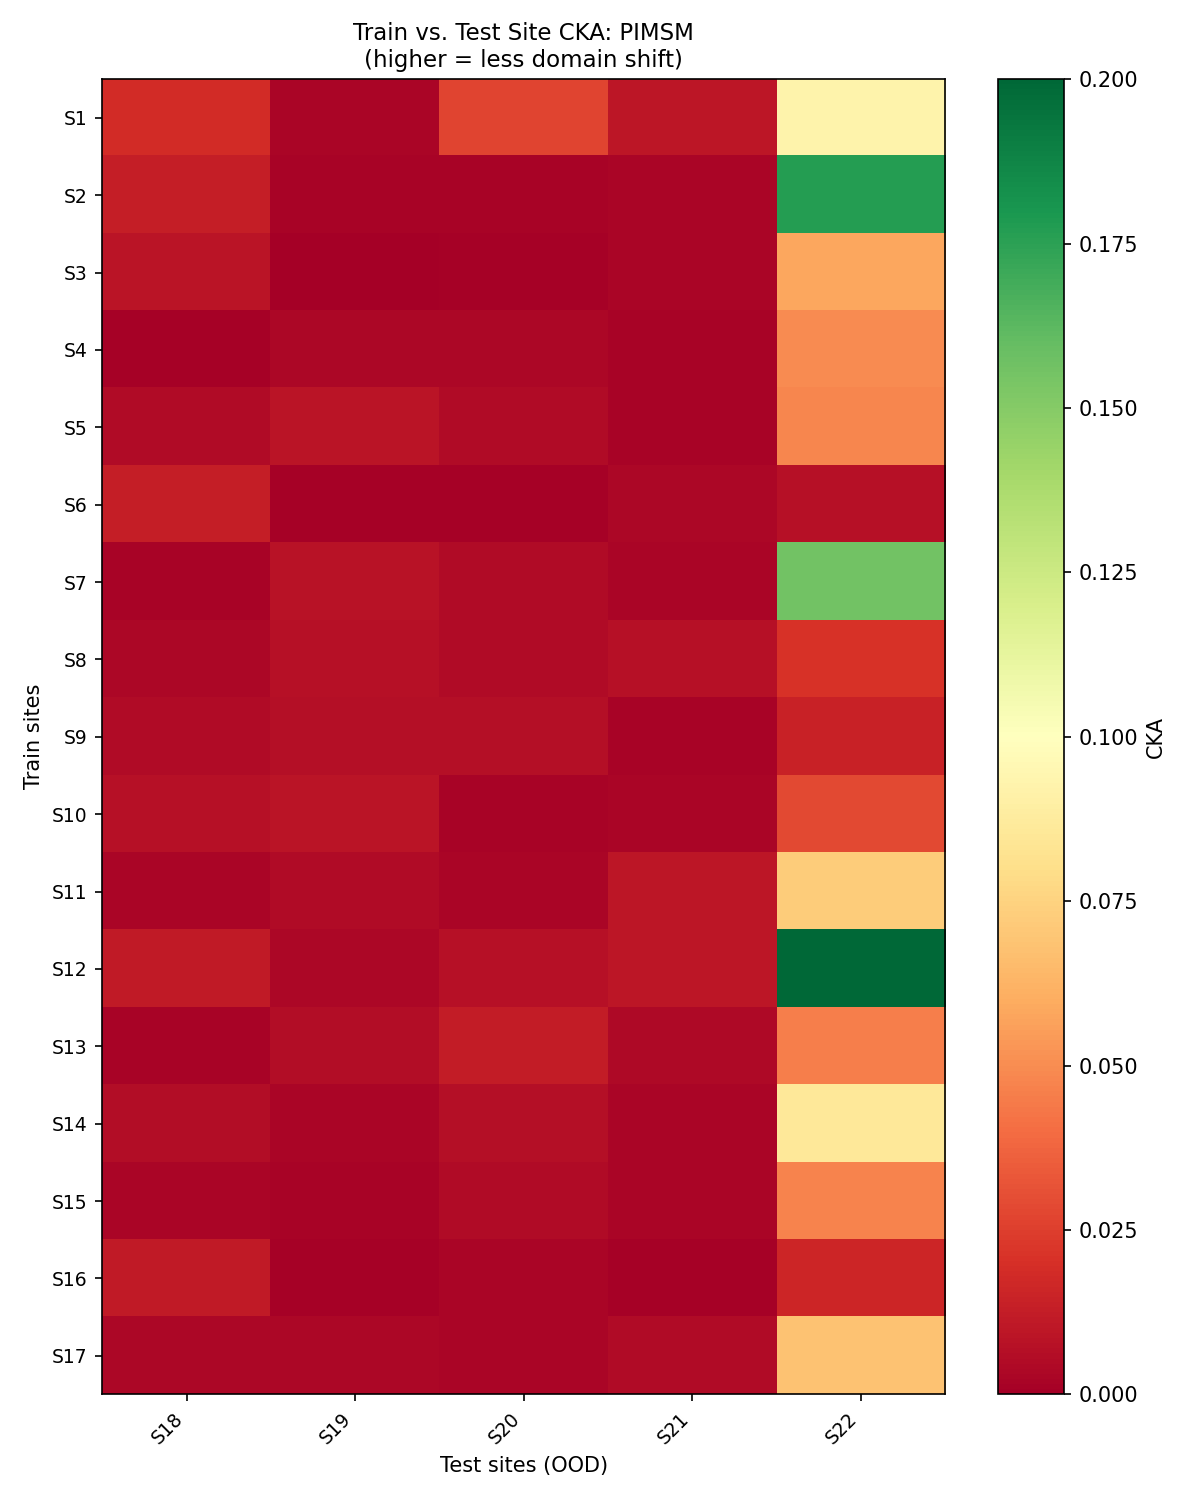
\includegraphics[width=0.235\textwidth]{figures/train_vs_test_cka_pimsm.png}\hfill
% 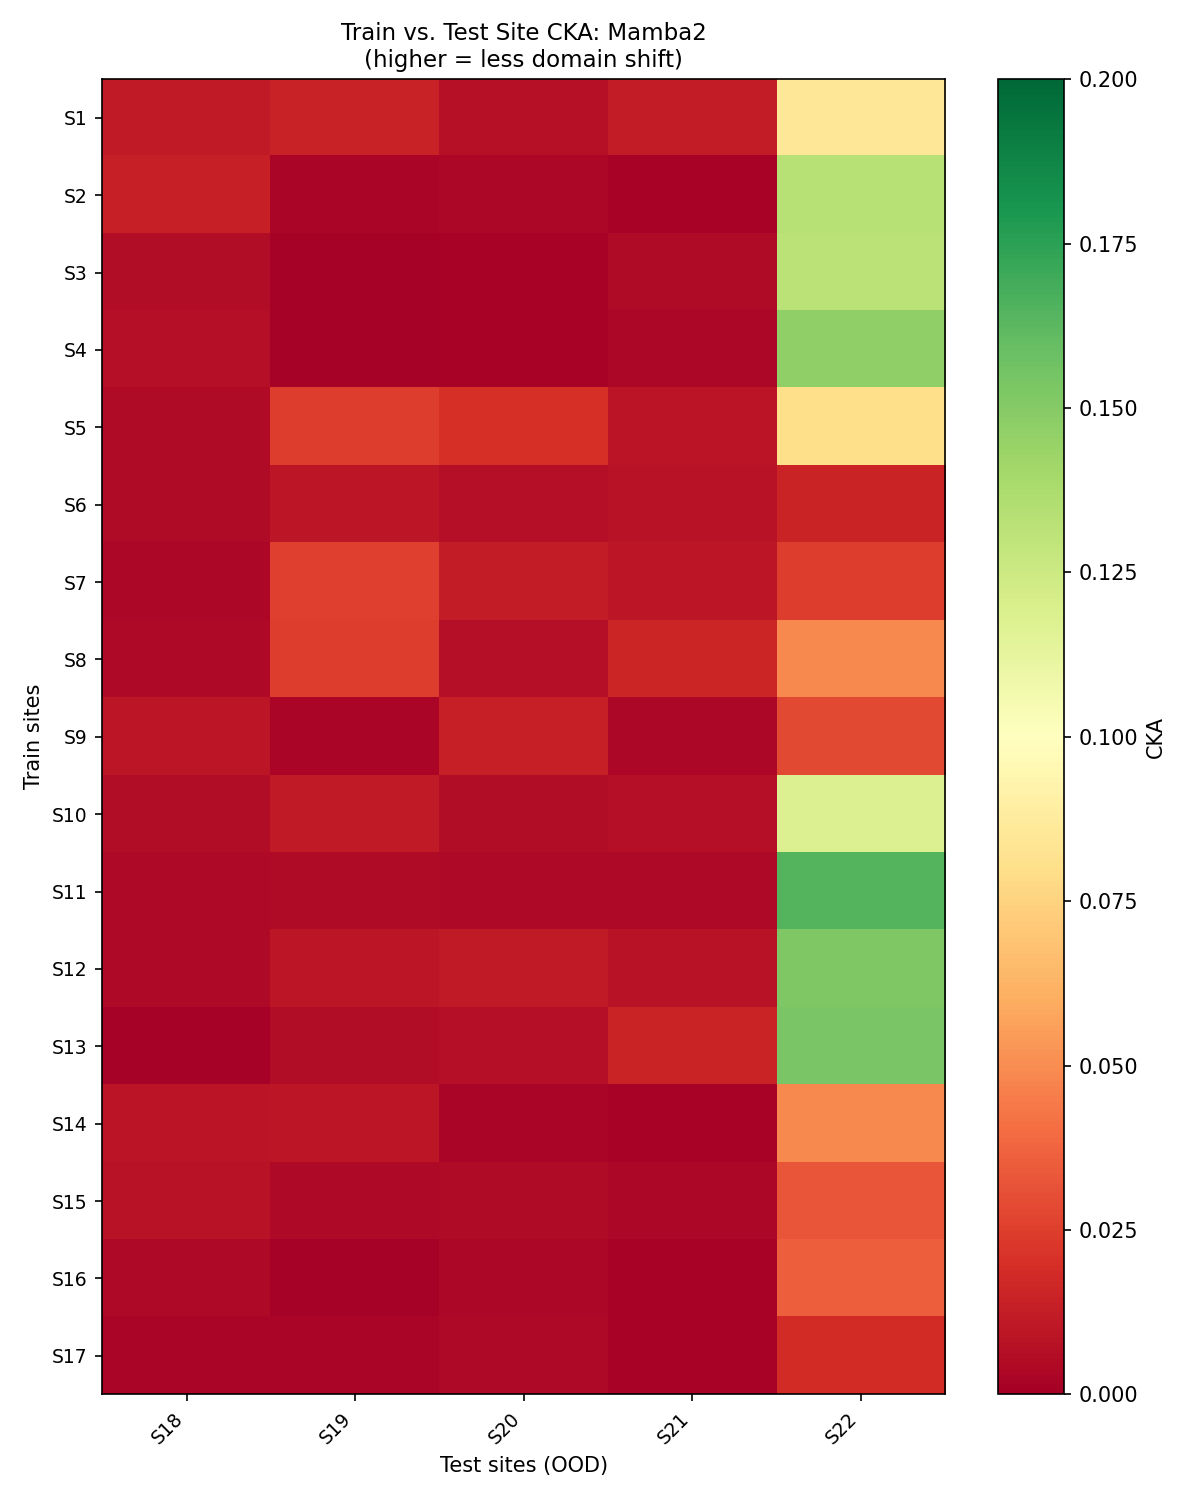
\includegraphics[width=0.235\textwidth]{figures/train_vs_test_cka_mamba2.png}\hfill
% 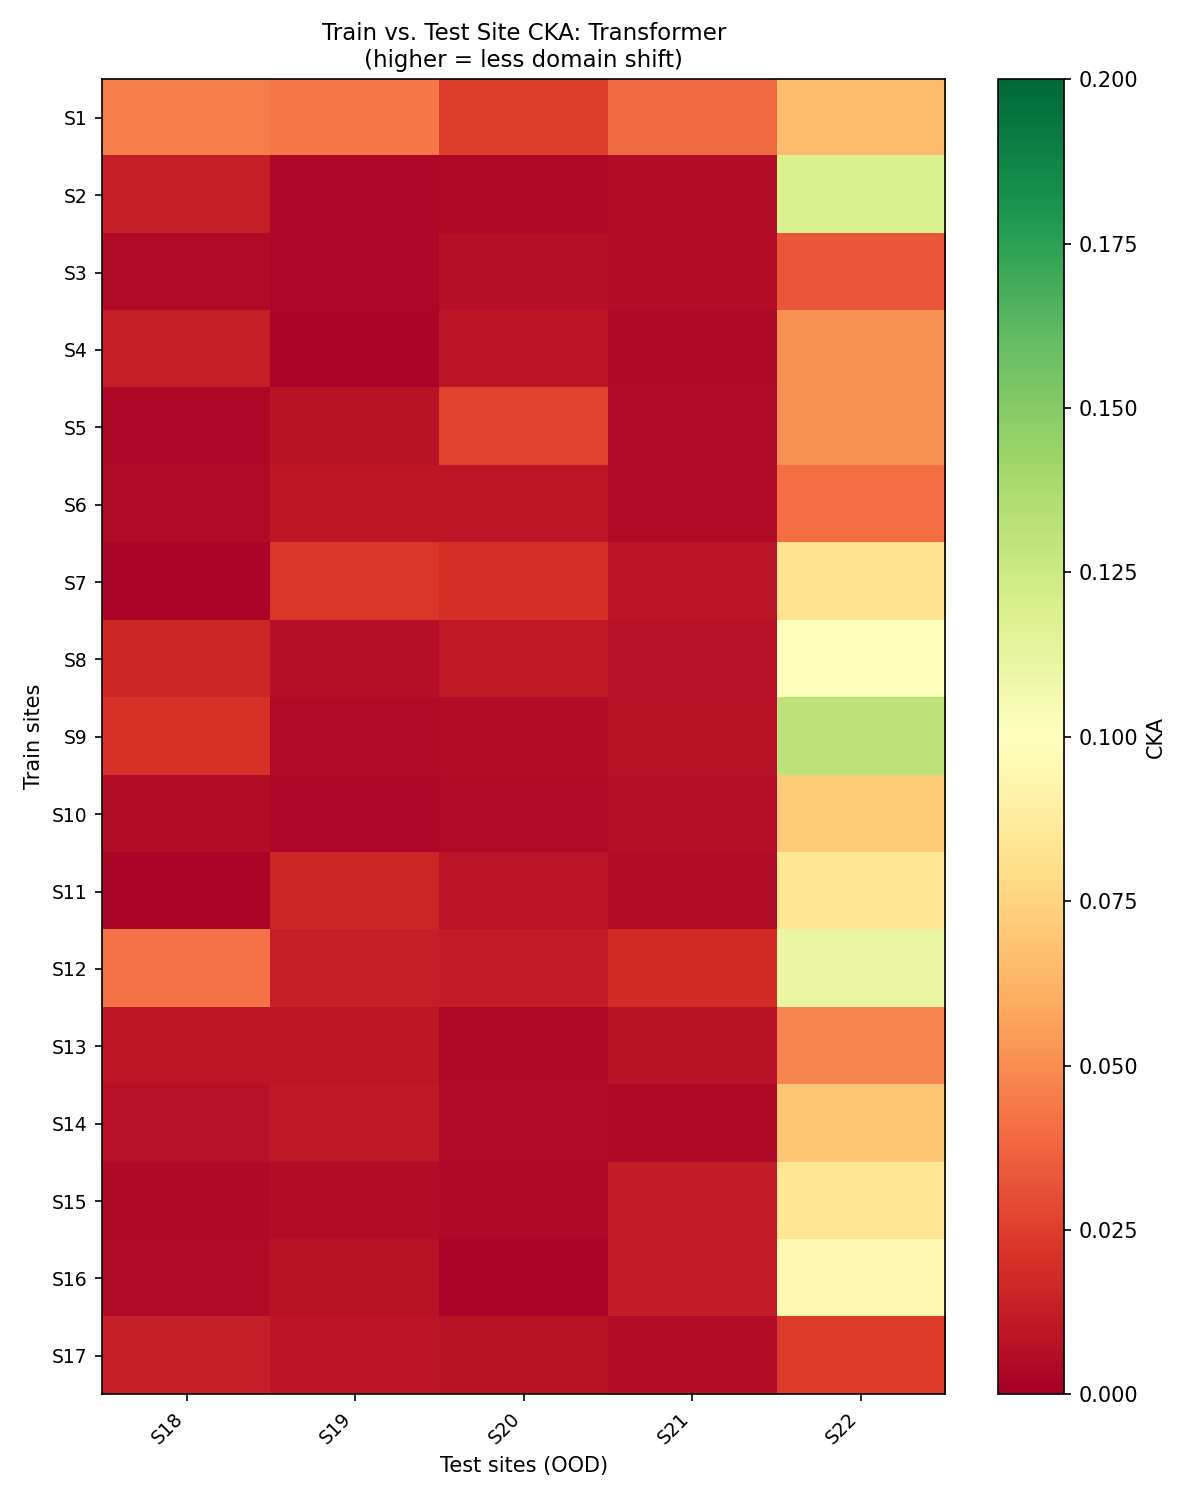
\includegraphics[width=0.235\textwidth]{figures/train_vs_test_cka_transformer.png}\hfill
% 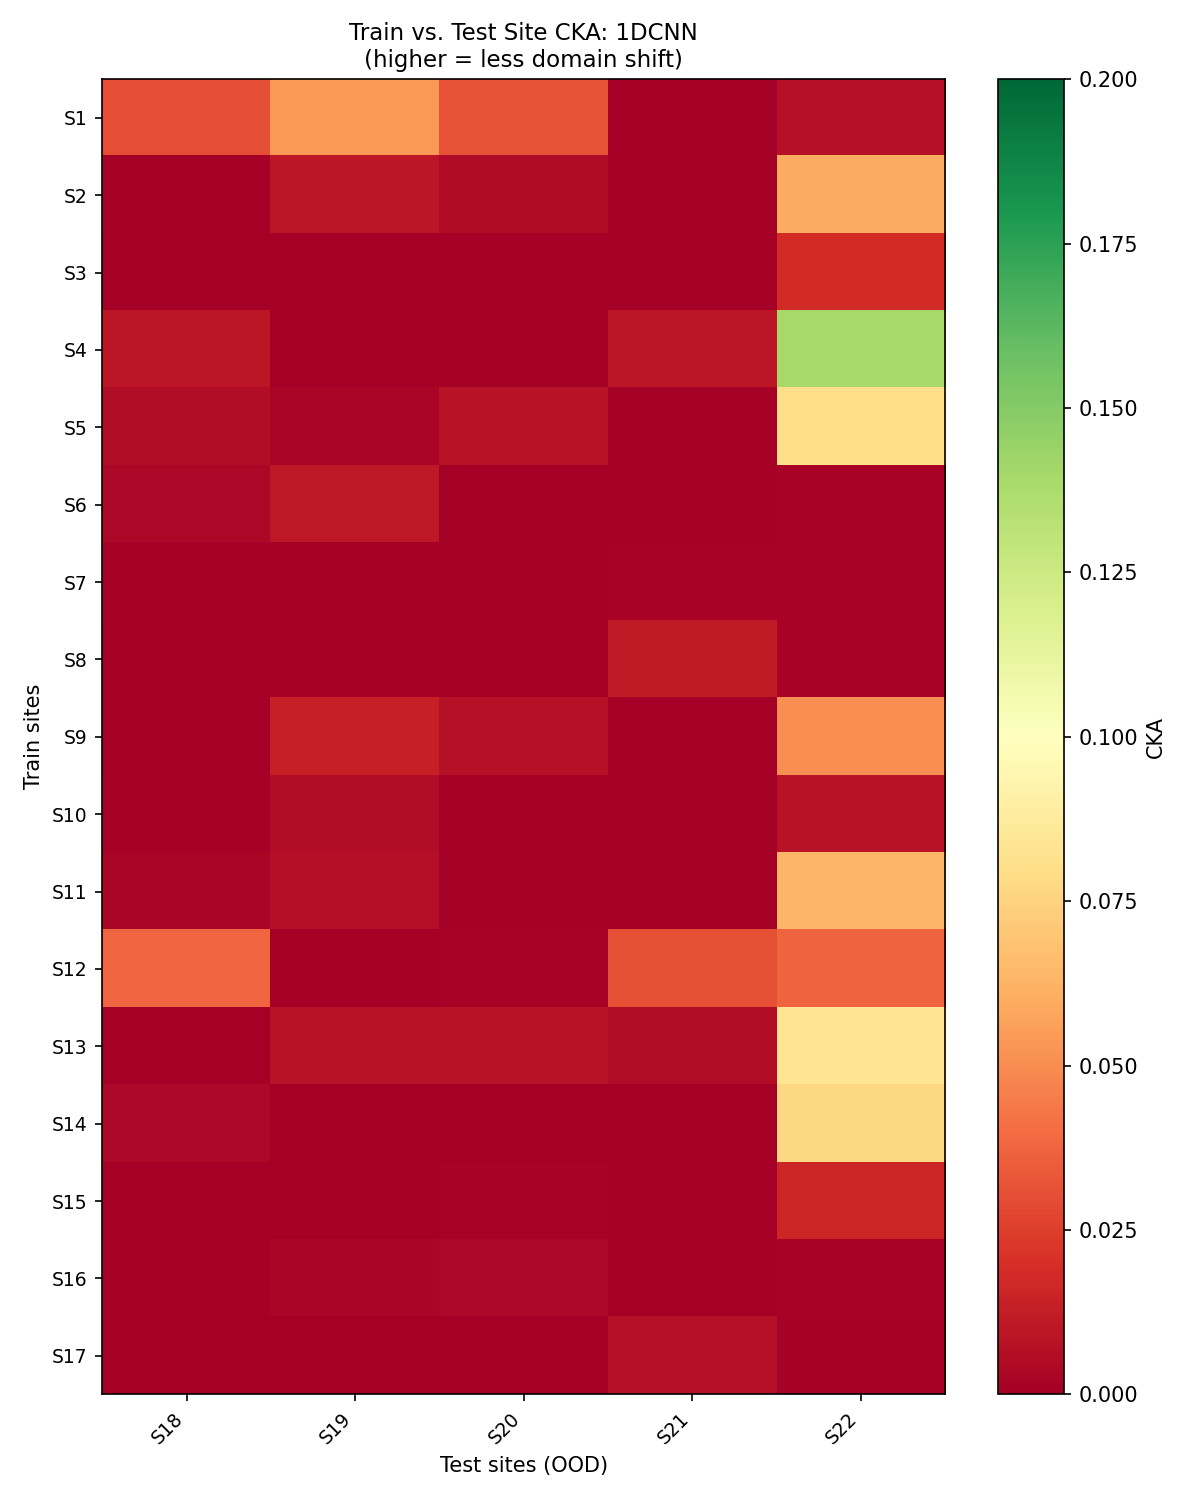
\includegraphics[width=0.235\textwidth]{figures/train_vs_test_cka_1dcnn.png}
% \caption{
% \textbf{Layer-wise linear CKA between train-site and held-out-site representations (ABCD resting-state).}
% Each panel corresponds to one architecture (PIMSM, Mamba2, Transformer, 1D-CNN). Higher CKA indicates more aligned geometry across the scanner-site split.
% }
% \label{fig:abcd_train_test_cka}
% \end{figure*}
% -----------------------------------------------------------------------

\section{HCP Motor Decoding under Temporal-Context Shift: Additional Details}
\label{sec:appx:hcp_tr_shift}

This appendix provides supporting detail for Section~\ref{sec:results:hcp_tr_shift}. The severe 2TR result is reported in the main text (Table~\ref{tab:drift2tr}); here we include the moderate 3TR table, drift intervention tables, scaling figures, and Figure~\ref{fig:tr_shift_stability}. As in the main text, SpectralHyperNet uses the full trial sequence for spectral calibration, while the SSM backbone receives the truncated early-window input.

\begin{table}[htbp]
\centering
\footnotesize
\begin{tabular}{lcccc}
\toprule
Model & Full trial & 3 TRs & CKA (Full trial$\leftrightarrow$3TR) & dCor (Full trial$\leftrightarrow$3TR) \\
\midrule
Mamba2 & $0.983\pm0.002$ & $0.931\pm0.010$ & $0.786\pm0.031$ & $0.817\pm0.025$ \\
1DCNN & $0.978\pm0.007$ & $0.874\pm0.001$ & $0.585\pm0.008$ & $0.658\pm0.001$ \\
Transformer & $0.982\pm0.006$ & $0.927\pm0.007$ & $0.839\pm0.019$ & $0.864\pm0.016$ \\
PIMSM (learnable $\Delta$) & $0.982\pm0.001$ & $0.937\pm0.004$ & $0.865\pm0.006$ & $0.881\pm0.005$ \\
PIMSM (random $\Delta$) & $0.983\pm0.004$ & $0.934\pm0.003$ & $0.846\pm0.026$ & $0.873\pm0.019$ \\
\midrule
\textbf{PIMSM} & $\mathbf{0.987\pm0.007}$ & $\mathbf{0.944\pm0.005}$ & $\mathbf{0.854\pm0.022}$ & $\mathbf{0.878\pm0.020}$ \\
\bottomrule
\end{tabular}
\caption{
\textbf{HCP motor decoding under moderate temporal-context truncation (full trial $\rightarrow$ 3 TRs).}
Values are mean $\pm$ std over three seeds.
}
\label{tab:drift3tr}
\end{table}


\paragraph{Drift intervention.}
We introduce explicit drift regularization for Mamba2: $\mathcal{L} = \mathcal{L}_{\text{task}} + \lambda D(z(x^{\text{full}}), z(x^{\text{trunc}}))$. This model (Mamba2+drift) improves representation stability and decoding accuracy under temporal-context truncation without degrading ID performance, supporting representation drift as a useful robustness target. PIMSM achieves comparable stability through architecture alone, without explicit shift supervision. See Tables~\ref{tab:drift_intervention_2tr} and~\ref{tab:drift_intervention_3tr}.

\paragraph{Scaling behavior.}
Larger PIMSM models exhibit increasingly stable representations under temporal-context truncation, whereas the single-scale SSM baseline shows smaller robustness gains from additional capacity (Figure~\ref{fig:scaling}). Additional WeightWatcher analysis (Section~\ref{sec:appx:weightwatcher}) provides complementary evidence that multi-scale structure helps preserve representation diversity.

\begin{figure}[htbp]
\centering
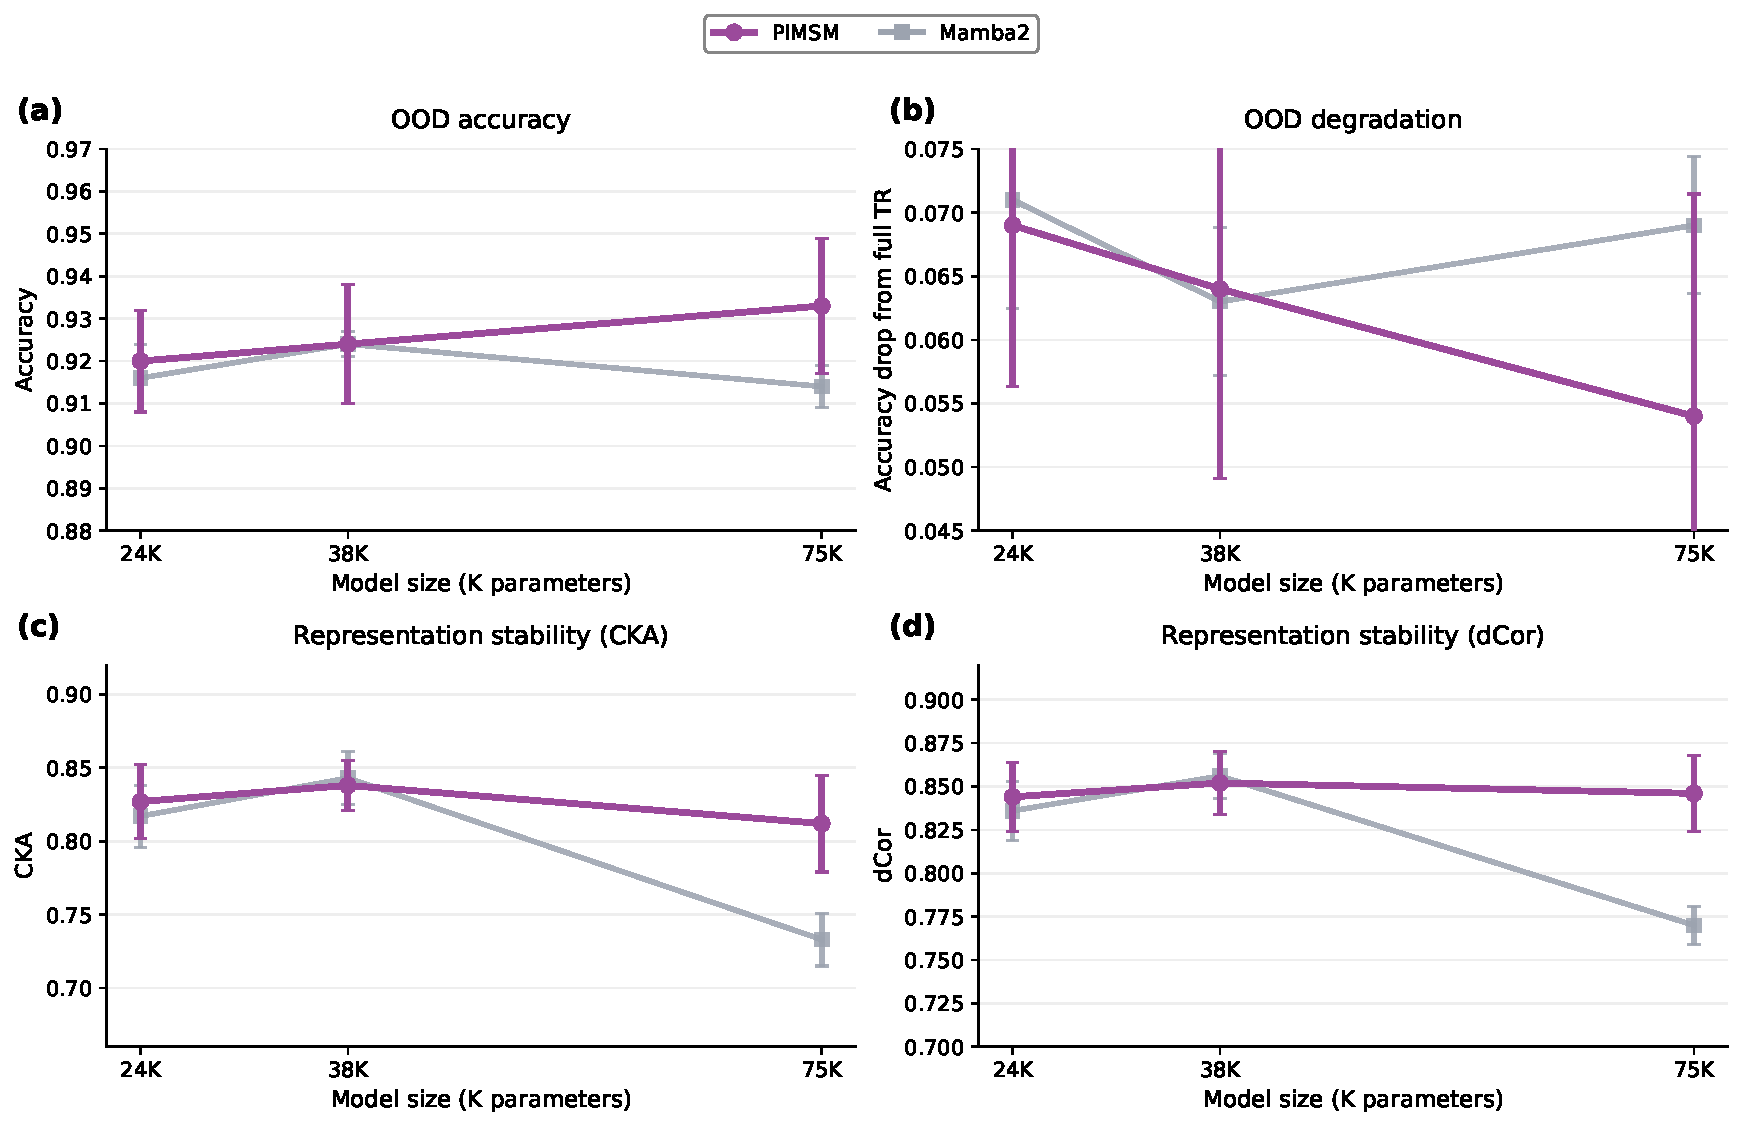
\includegraphics[width=\textwidth]{figures/PIMSM_Fig3.pdf}
\caption{
\textbf{Scaling behavior under temporal-context truncation (full trial $\rightarrow$ 2TR).}
(a) Decoding accuracy vs model size. (b) Accuracy drop relative to full-trial input. (c--d) CKA and dCor between full-trial and 2TR representations.
}
\label{fig:scaling}
\end{figure}

\begin{table}[htbp]
\centering
\footnotesize
\begin{tabular}{lcccc}
\toprule
Model & Full trial & 2 TRs & CKA (Full trial$\leftrightarrow$2TR) & dCor (Full trial$\leftrightarrow$2TR) \\
\midrule
PIMSM & 0.987$\pm$0.007 & 0.933$\pm$0.016 & 0.812$\pm$0.033 & 0.846$\pm$0.022 \\
Mamba2+drift & 0.987$\pm$0.004 & 0.923$\pm$0.009 & 0.837$\pm$0.021 & 0.854$\pm$0.019 \\
\bottomrule
\end{tabular}
\caption{Drift intervention: full trial $\rightarrow$ 2 TR. Values are mean $\pm$ std over three seeds.}
\label{tab:drift_intervention_2tr}
\end{table}

\begin{table}[htbp]
\centering
\footnotesize
\begin{tabular}{lcccc}
\toprule
Model & Full trial & 3 TRs & CKA (Full trial$\leftrightarrow$3TR) & dCor (Full trial$\leftrightarrow$3TR) \\
\midrule
PIMSM & 0.987$\pm$0.007 & 0.944$\pm$0.005 & 0.854$\pm$0.022 & 0.878$\pm$0.020 \\
Mamba2+drift & 0.987$\pm$0.004 & 0.939$\pm$0.011 & 0.854$\pm$0.036 & 0.879$\pm$0.025 \\
\bottomrule
\end{tabular}
\caption{Drift intervention: full trial $\rightarrow$ 3 TR. Values are mean $\pm$ std over three seeds.}
\label{tab:drift_intervention_3tr}
\end{table}


\section{Low-Resource Generalization: Additional Details}
\label{sec:appx:data_scarce}

Results are reported in Table~\ref{tab:data_scarce} and Section~\ref{sec:results:data_scarce} of the main text.


\section{WeightWatcher Analysis: Layer-wise Power-Law Exponents}
\label{sec:appx:weightwatcher}

\begin{figure}[htbp]
\centering
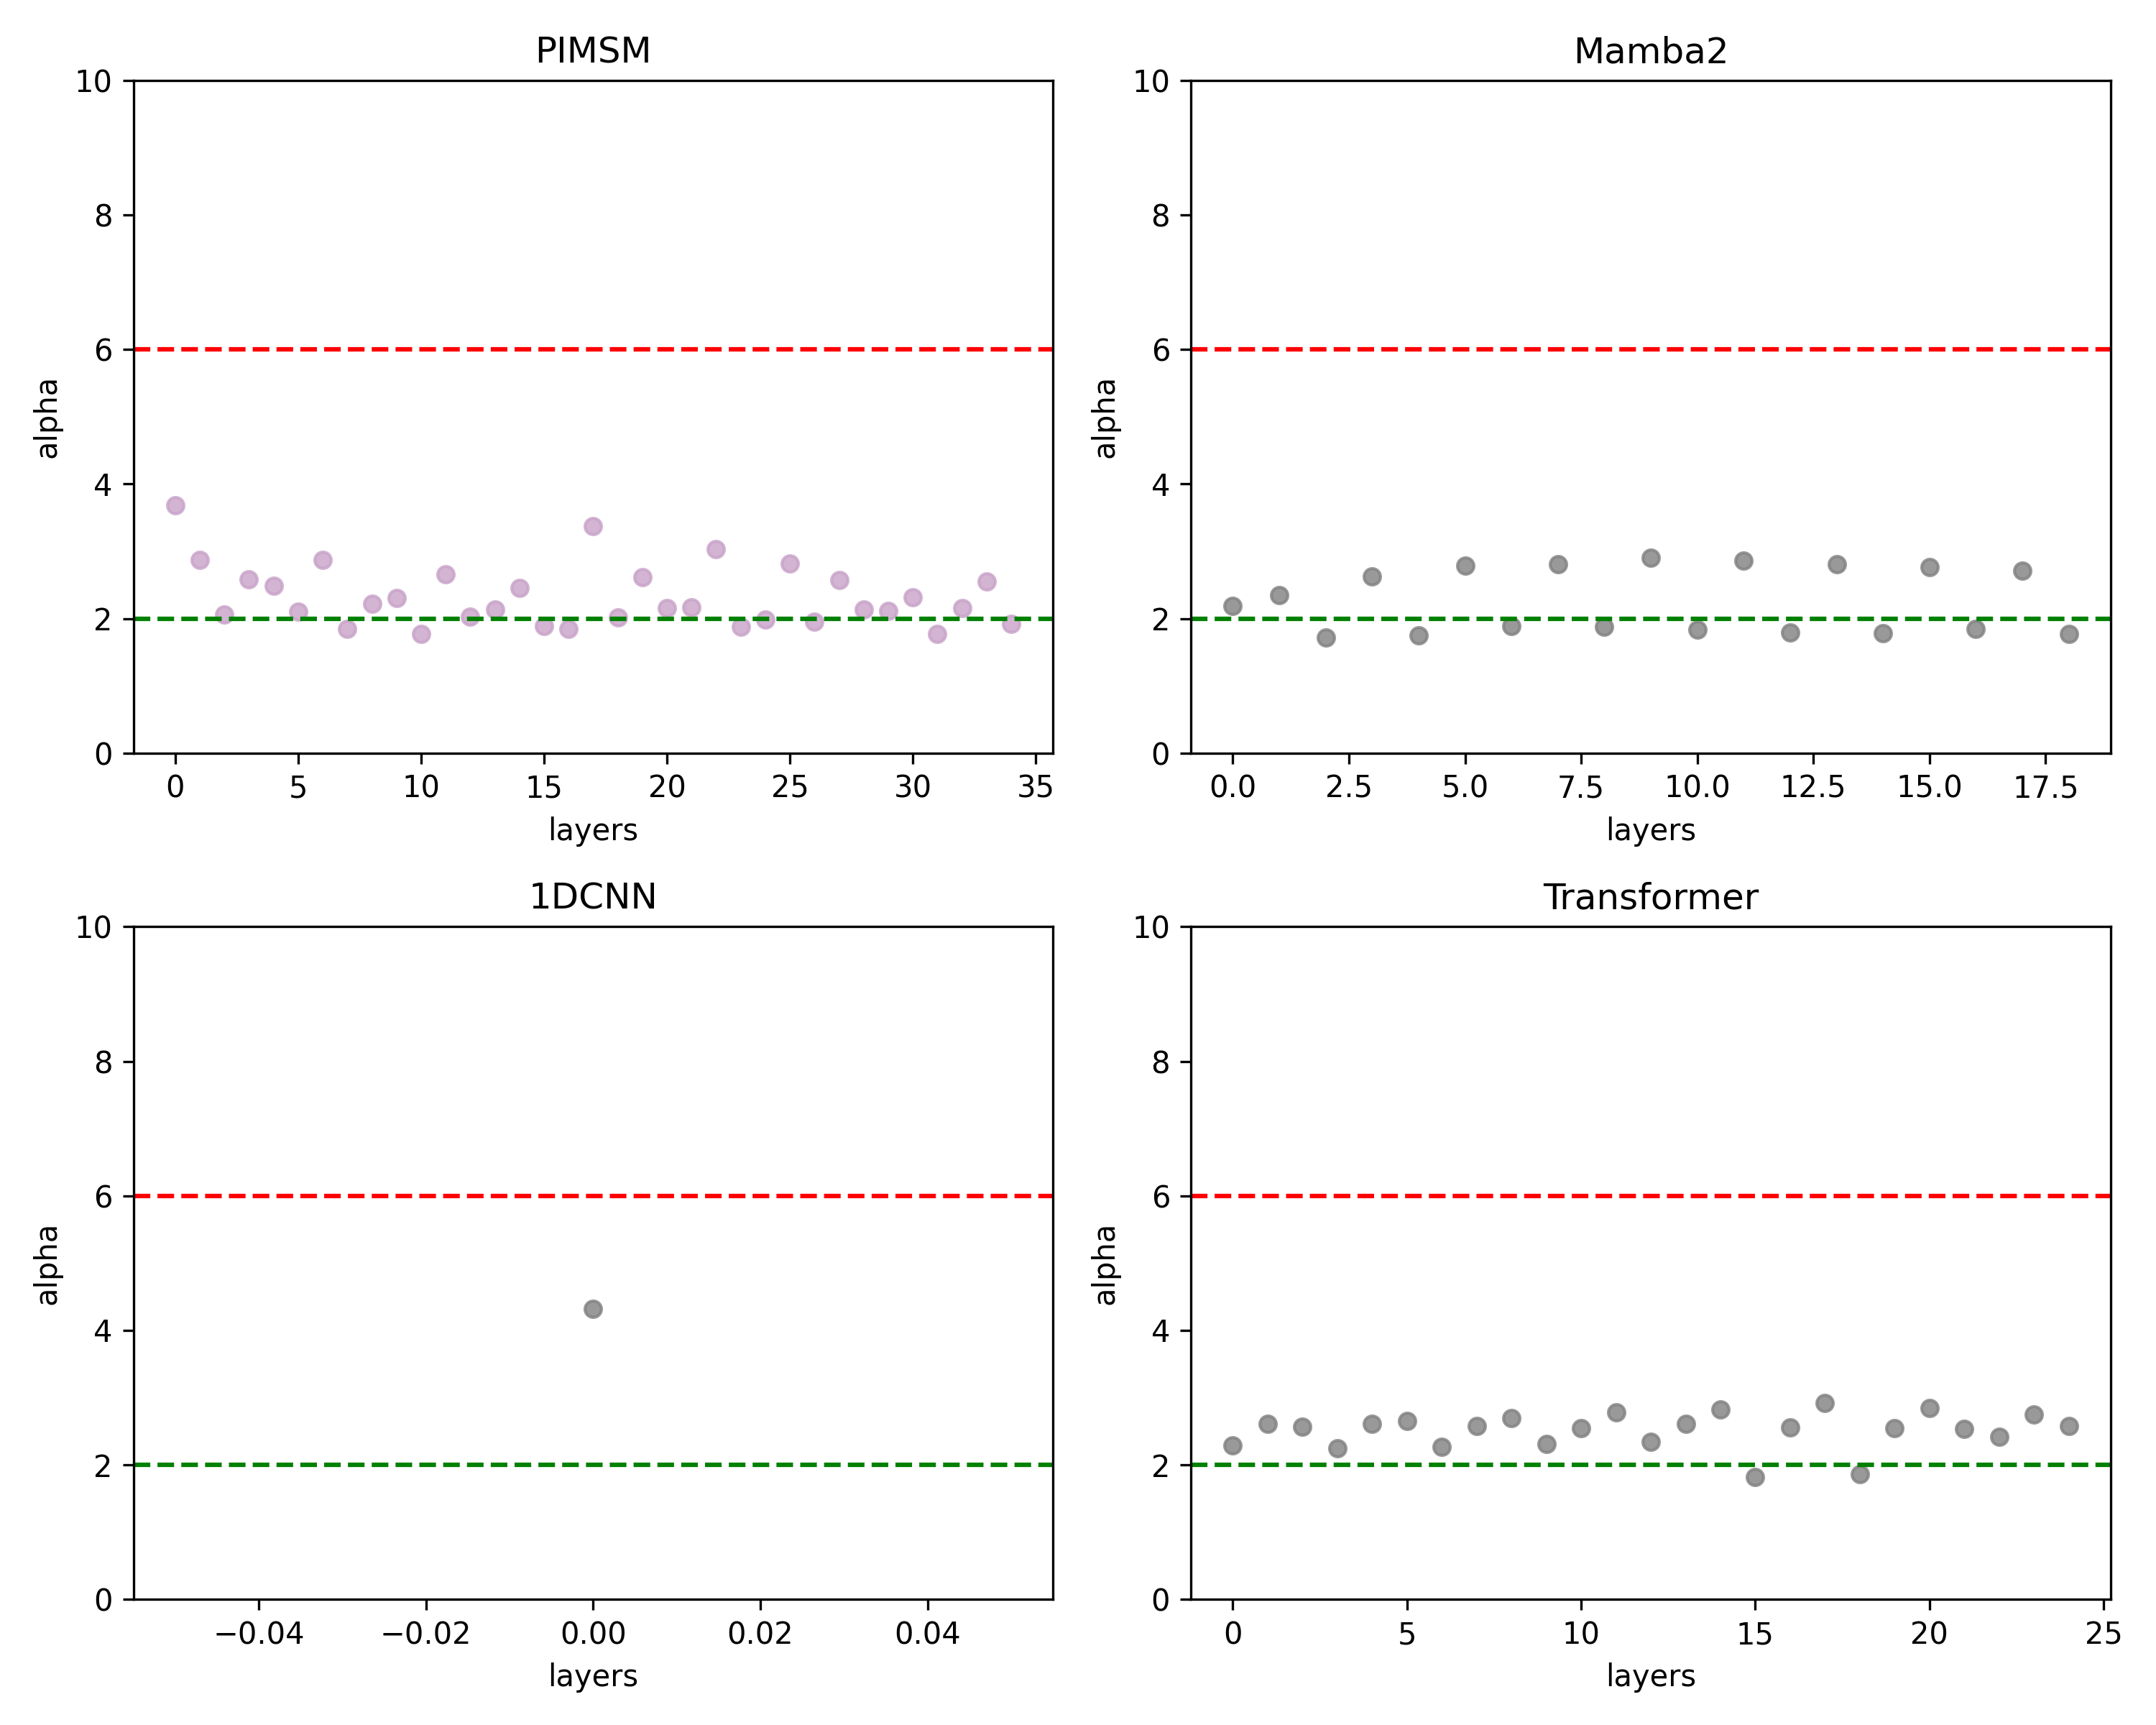
\includegraphics[width=0.85\linewidth]{figures/weightwatcher_motor_full_TR.png}
\caption{
\textbf{WeightWatcher layer-wise $\alpha$ distributions under full-trial input (HCP motor task fMRI).}
Each point represents the power-law exponent $\alpha$ of the empirical spectral density of a weight matrix.
The red dashed line ($\alpha = 6$) marks the boundary above which weights are statistically indistinguishable from random matrices;
the green dashed line ($\alpha = 2$) indicates the onset of over-training.
PIMSM exhibits heterogeneous $\alpha$ values (1.77--3.69) spread across a wide range, indicating that different layers operate at distinct feature-complexity regimes.
Mamba2 and Transformer concentrate near $\alpha \approx 2$, suggesting that most layers have reached training saturation.
1D-CNN has only one analyzable layer (remaining layers contain weight matrices too small for reliable spectral fitting).
}
\label{fig:ww_full_tr}
\end{figure}

\begin{figure}[htbp]
\centering
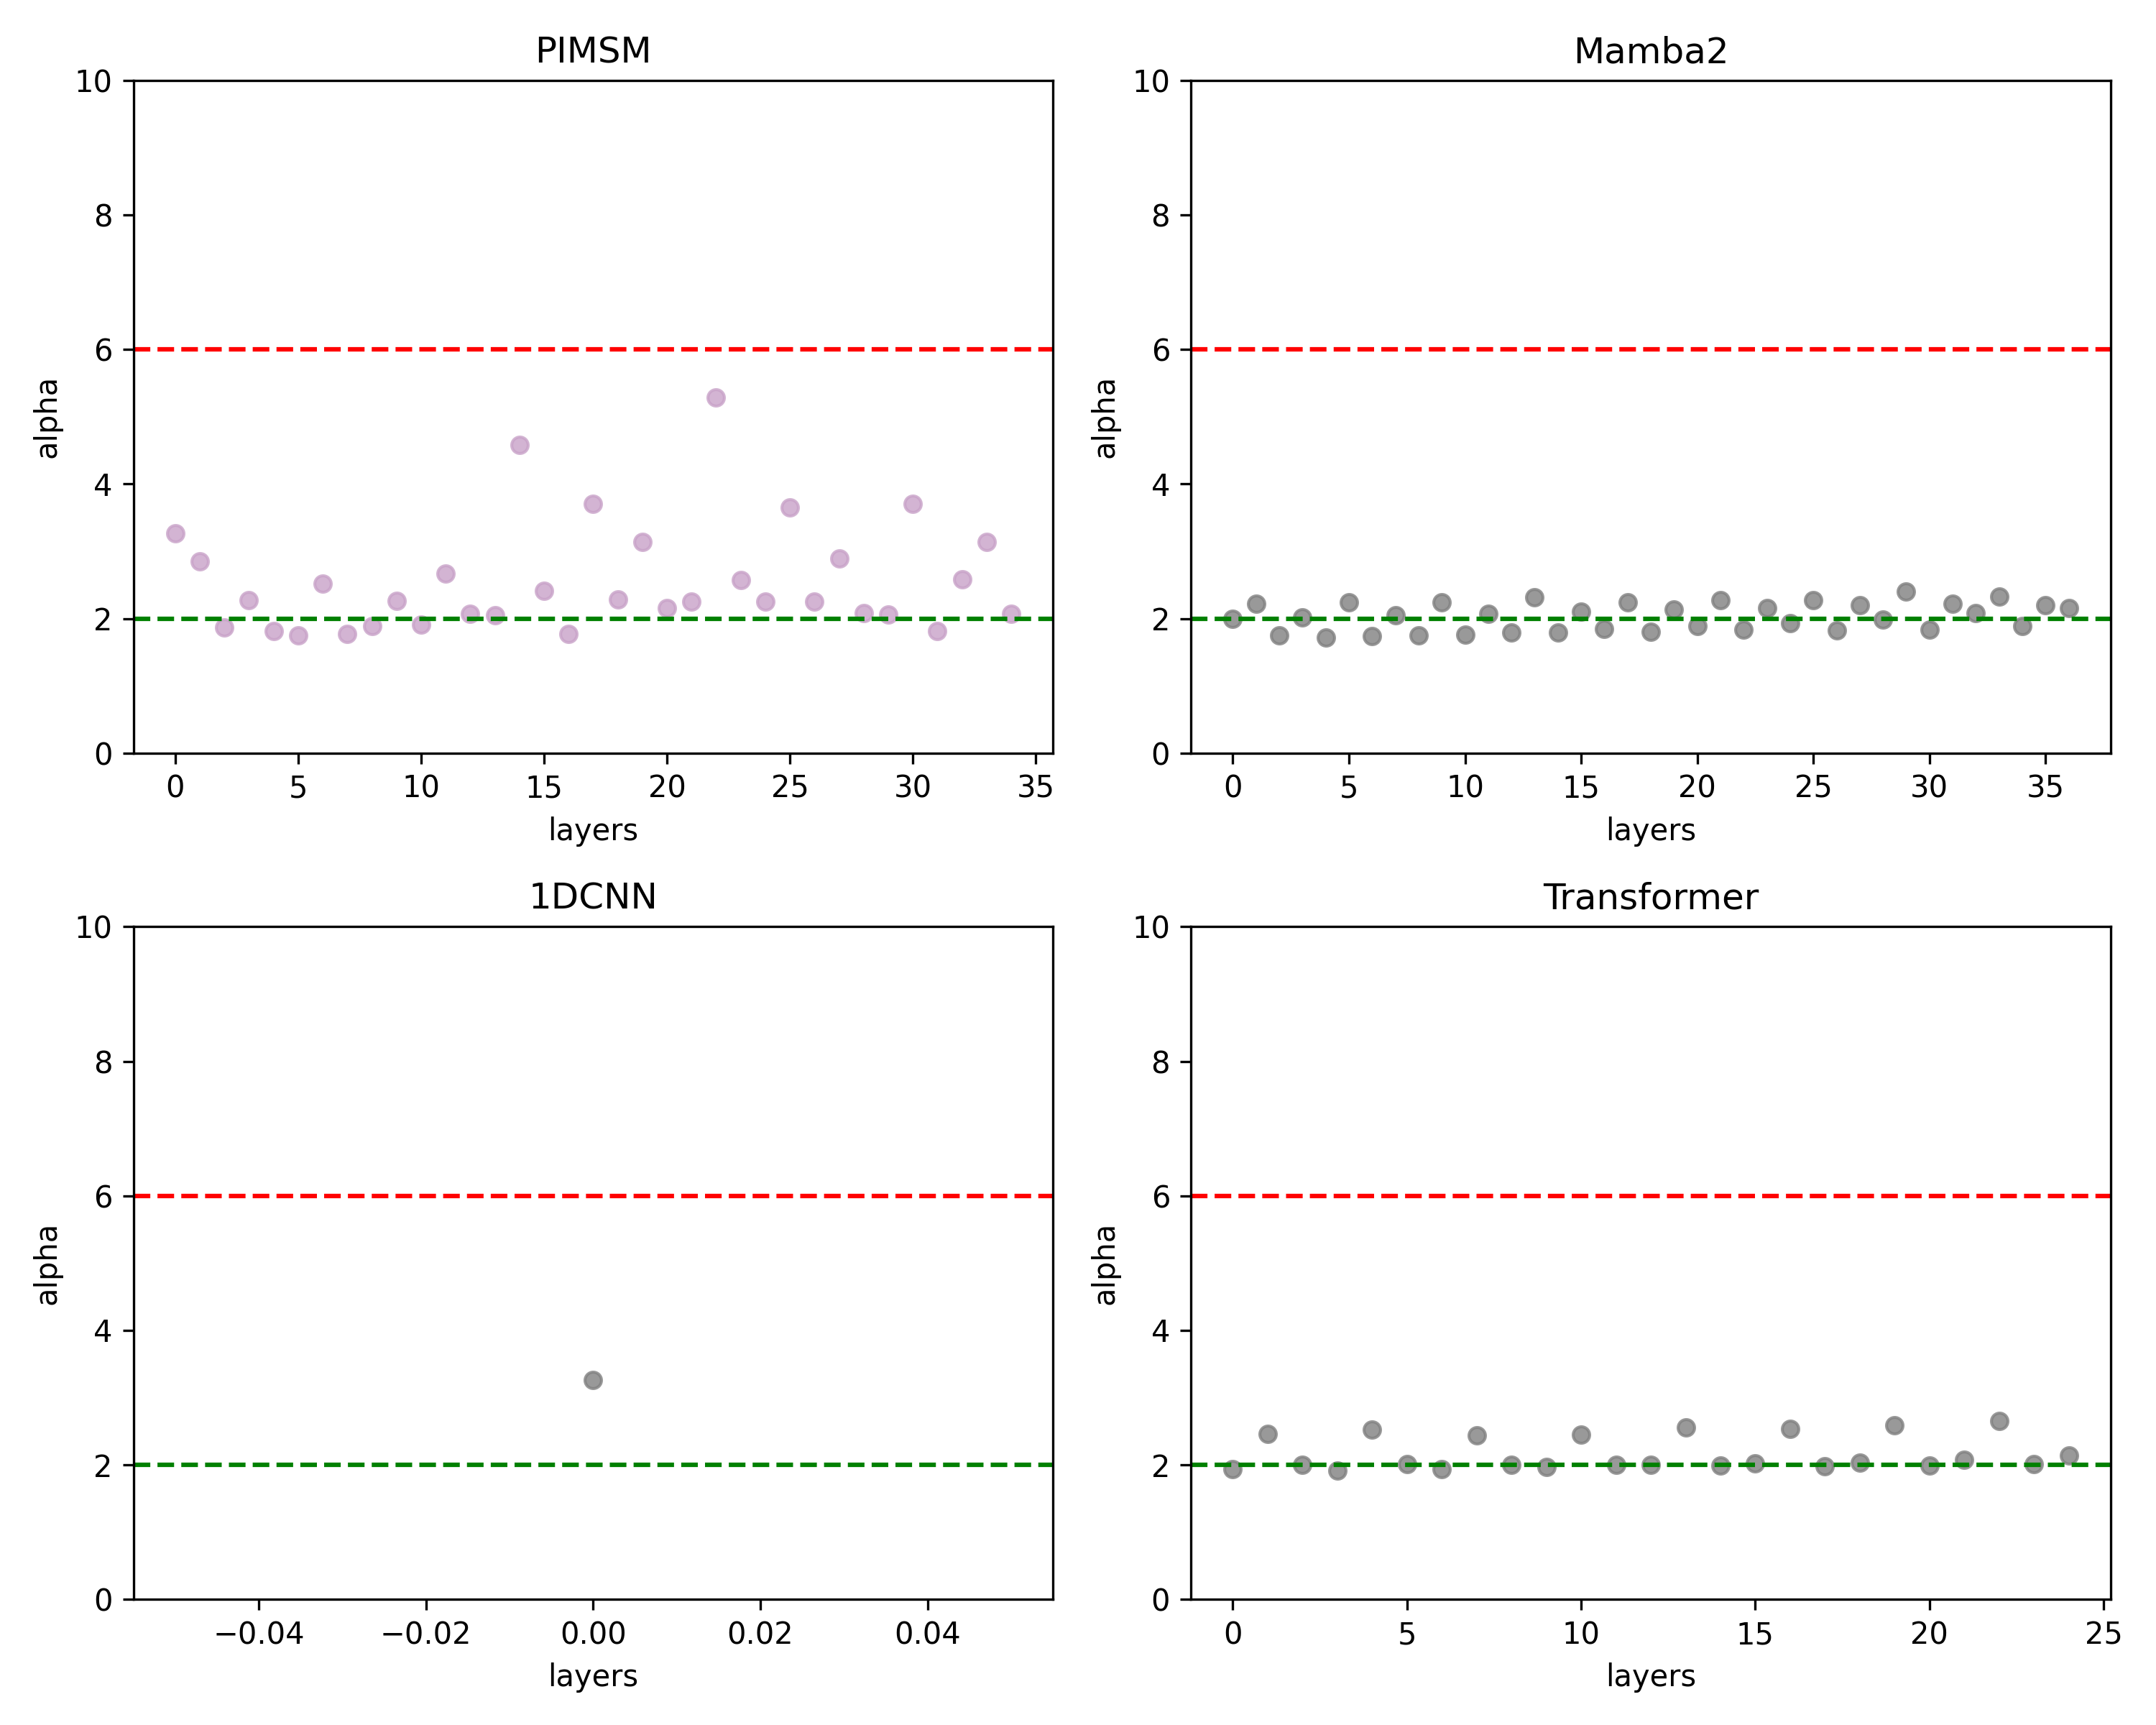
\includegraphics[width=0.85\linewidth]{figures/weightwatcher_motor_2TR.png}
\caption{
\textbf{WeightWatcher layer-wise $\alpha$ distributions under 2 TR early-window condition (extreme temporal truncation).}
Under the 2 TR condition---an extreme data-scarce scenario in which only two time points are available per trial---PIMSM maintains a wide $\alpha$ spread (1.75--5.29), indicating that layer-wise representational diversity is preserved despite the severely reduced input.
In contrast, Mamba2 concentrates more uniformly near $\alpha \approx 2$ (all 37 analyzable layers saturate simultaneously), suggesting greater representation homogenization when learning signals are scarce.
The Transformer retains a similar distribution to its full-trial counterpart but with reduced variance.
}
\label{fig:ww_2tr}
\end{figure}

WeightWatcher~\citep{martin2021predicting} quantifies the implicit self-regularization of each weight matrix by fitting the tail of its empirical spectral density (ESD) to a power law $\rho(\lambda) \propto \lambda^{-\alpha}$.
Matrices with $\alpha \in [2, 6]$ are considered \emph{well-trained}: $\alpha < 2$ indicates over-training (insufficient regularization), and $\alpha > 6$ indicates that the matrix is statistically indistinguishable from a random initialization.
Note that WeightWatcher analyzes 2D matrices only; 4D convolution tensors (as in 1D-CNN) are excluded except for the final linear layer.

\paragraph{Full-trial condition (Figure~\ref{fig:ww_full_tr}).}
Under the standard full-trial condition, PIMSM exhibits $\alpha \in [1.77, 3.69]$ with notable layer-to-layer variation.
This heterogeneity reflects the multi-scale inductive bias of the architecture: different PIMSM layers specialize to capture temporal correlations at different scales, resulting in layers with distinct implicit regularization properties.
In contrast, Mamba2 and Transformer accumulate near $\alpha \approx 2.0$, indicating that most layers are in a saturated learning state.
These models may be efficiently encoding in-distribution patterns but leave little representational capacity available for adaptation under shift.

\paragraph{2 TR early-window condition (Figure~\ref{fig:ww_2tr}).}
Under the extreme 2 TR condition, PIMSM's $\alpha$ distribution widens further (1.75--5.29).
Rather than homogenizing under reduced input, the multi-scale architecture preserves layer-wise role differentiation---deeper layers tend toward higher $\alpha$ (less specialized), while early layers remain well-fitted---suggesting that the model gracefully degrades without global collapse.
Mamba2, by contrast, narrows its $\alpha$ distribution toward $\approx 2.0$ with near-zero variance across all 37 analyzable layers, consistent with representation homogenization under information-sparse inputs.
The Transformer shows moderate variance reduction but remains closer to its full-trial distribution, perhaps due to the global attention mechanism retaining some diversity.

\paragraph{Interpretation.}
These layer-wise spectral analyses provide weight-level corroboration for the conclusion drawn from CKA and distance correlation measurements:
PIMSM's multi-scale structure actively resists representation collapse when temporal context is severely reduced.
The preserved heterogeneity of $\alpha$ values across layers suggests that the physics-informed multi-scale parameterization may act as an implicit regularizer that discourages collapse to a single dominant feature regime under severe temporal truncation.


\section{Effect of Pretraining: Finetuning and Linear Probing}
\label{sec:appx:pretrain}

\subsection{Finetuning from Resting-State Pretraining}

\begin{table}[htbp]
\centering
\footnotesize
\begin{tabular}{lccccc}
\toprule
Model & From Scratch & Full trial & 2 TRs & CKA & dCor \\
\midrule
PIMSM & $0.987 \pm 0.007$ & $0.987 \pm 0.004$ & $\mathbf{0.937 \pm 0.009}$ & $\mathbf{0.867 \pm 0.004}$ & $\mathbf{0.889 \pm 0.009}$ \\
Mamba2 & $0.983 \pm 0.002$ & $0.987 \pm 0.007$ & $0.933 \pm 0.011$ & $0.847 \pm 0.024$ & $0.860 \pm 0.024$ \\
\midrule
Model & From Scratch & Full trial & 3 TRs & CKA & dCor \\
\midrule
PIMSM & $0.987 \pm 0.007$ & $0.987 \pm 0.004$ & $\mathbf{0.949 \pm 0.012}$ & $\mathbf{0.878 \pm 0.005}$ & $\mathbf{0.899 \pm 0.002}$ \\
Mamba2 & $0.983 \pm 0.002$ & $0.987 \pm 0.007$ & $0.944 \pm 0.006$ & $0.874 \pm 0.010$ & $0.887 \pm 0.011$ \\
\bottomrule
\end{tabular}
\caption{
Effect of self-supervised pretraining on resting-state fMRI followed by finetuning on HCP motor task fMRI.
Values are mean $\pm$ std over three seeds.
Representation similarity (CKA, dCor) is measured between full-trial and early-window inputs.
Pretraining improves shift robustness for both models, with PIMSM retaining a small but consistent advantage in representation stability.
}
\label{tab:pretrain_finetune}
\end{table}

We evaluate whether self-supervised pretraining on resting-state fMRI improves downstream shift robustness when models are subsequently finetuned on motor task fMRI (Table~\ref{tab:pretrain_finetune}).
Pretraining raises shifted-condition accuracy and representation similarity relative to training from scratch for both PIMSM and Mamba2.
Under the 2 TR condition, pretrained PIMSM achieves $0.937 \pm 0.009$ versus $0.933 \pm 0.011$ for pretrained Mamba2; pretrained PIMSM also retains higher CKA ($0.867 \pm 0.004$) and dCor ($0.889 \pm 0.009$).
Under the 3 TR condition, pretrained PIMSM reaches $0.949 \pm 0.012$ versus $0.944 \pm 0.006$ for Mamba2.
These margins are consistent but modest, suggesting that the primary benefit of pretraining lies in improving representation stability under shift rather than raising the absolute performance ceiling.

\subsection{Linear Probing Evaluation}

\begin{table}[htbp]
\centering
\footnotesize
\begin{tabular}{lccccc}
\toprule
Model & From Scratch & Full trial & 2 TRs & CKA & dCor \\
\midrule
PIMSM & $0.987 \pm 0.007$ & $0.934 \pm 0.015$ & $\mathbf{0.748 \pm 0.003}$ & $0.444 \pm 0.029$ & $\mathbf{0.469 \pm 0.020}$ \\
Mamba2 & $0.983 \pm 0.002$ & $\mathbf{0.936 \pm 0.015}$ & $0.730 \pm 0.015$ & $\mathbf{0.448 \pm 0.041}$ & $0.462 \pm 0.036$ \\
\midrule
Model & From Scratch & Full trial & 3 TRs & CKA & dCor \\
\midrule
PIMSM & $0.987 \pm 0.007$ & $0.934 \pm 0.015$ & $\mathbf{0.791 \pm 0.027}$ & $0.470 \pm 0.032$ & $\mathbf{0.489 \pm 0.026}$ \\
Mamba2 & $0.983 \pm 0.002$ & $\mathbf{0.936 \pm 0.015}$ & $0.767 \pm 0.023$ & $\mathbf{0.475 \pm 0.042}$ & $0.484 \pm 0.035$ \\
\bottomrule
\end{tabular}
\caption{
Linear probing evaluation of pretrained models on HCP motor task fMRI.
Values are mean $\pm$ std over three seeds.
The backbone is frozen and only a linear classifier is trained.
CKA and dCor are measured between full-trial and early-window representations of the frozen backbone.
Both models achieve comparable full-trial accuracy ($\approx 0.93$), but PIMSM maintains slightly higher shifted-condition accuracy under 2 TR and 3 TR conditions.
}
\label{tab:linear_probe}
\end{table}

Under strict linear probing, both PIMSM and Mamba2 achieve similar full-trial accuracy ($\approx 0.93$).
Shifted-condition accuracy drops substantially for both models relative to the finetuning setting (Table~\ref{tab:pretrain_finetune}), reflecting the difficulty of adapting frozen representations to temporal-resolution shift via a linear readout alone.
PIMSM maintains a consistent advantage: $0.748 \pm 0.003$ vs.\ $0.730 \pm 0.015$ at 2 TR, and $0.791 \pm 0.027$ vs.\ $0.767 \pm 0.023$ at 3 TR.
CKA values under the frozen setting are substantially lower than under finetuning, suggesting that the full representational benefit of physics-informed pretraining is realized during downstream adaptation rather than through passively linearly separable representations.
These results are consistent with the view that multi-scale temporal modeling improves the plasticity of learned features during finetuning rather than directly encoding task geometry.


\section{Piecewise Power-Law Spectra Across Datasets}
\label{sec:appx:psd_multifractal}

\begin{figure}[htbp]
\centering
\begin{minipage}[b]{0.49\linewidth}
  \centering
  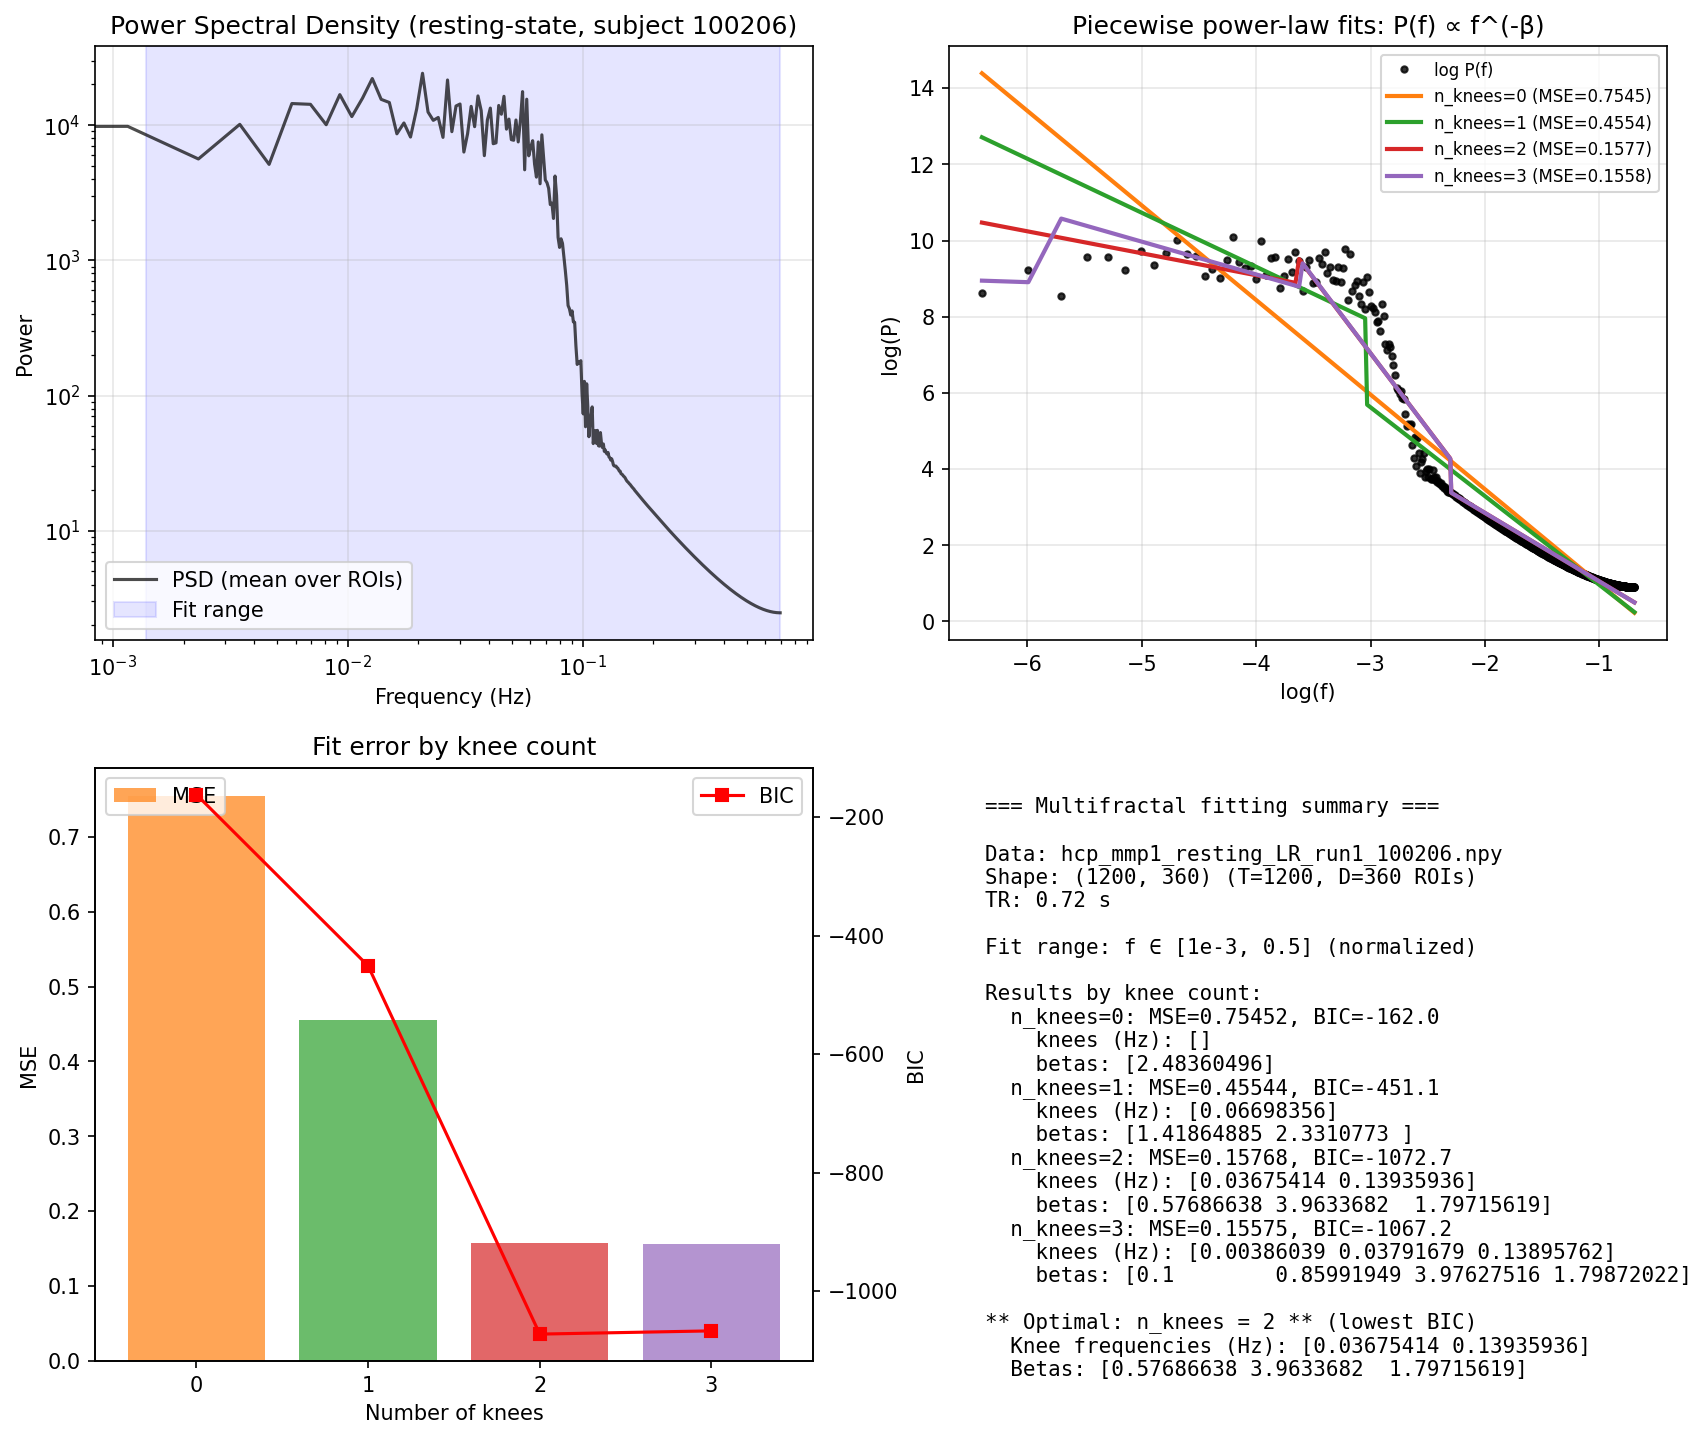
\includegraphics[width=\linewidth]{figures/resting_psd_multifractal.png}
\end{minipage}
\hfill
\begin{minipage}[b]{0.49\linewidth}
  \centering
  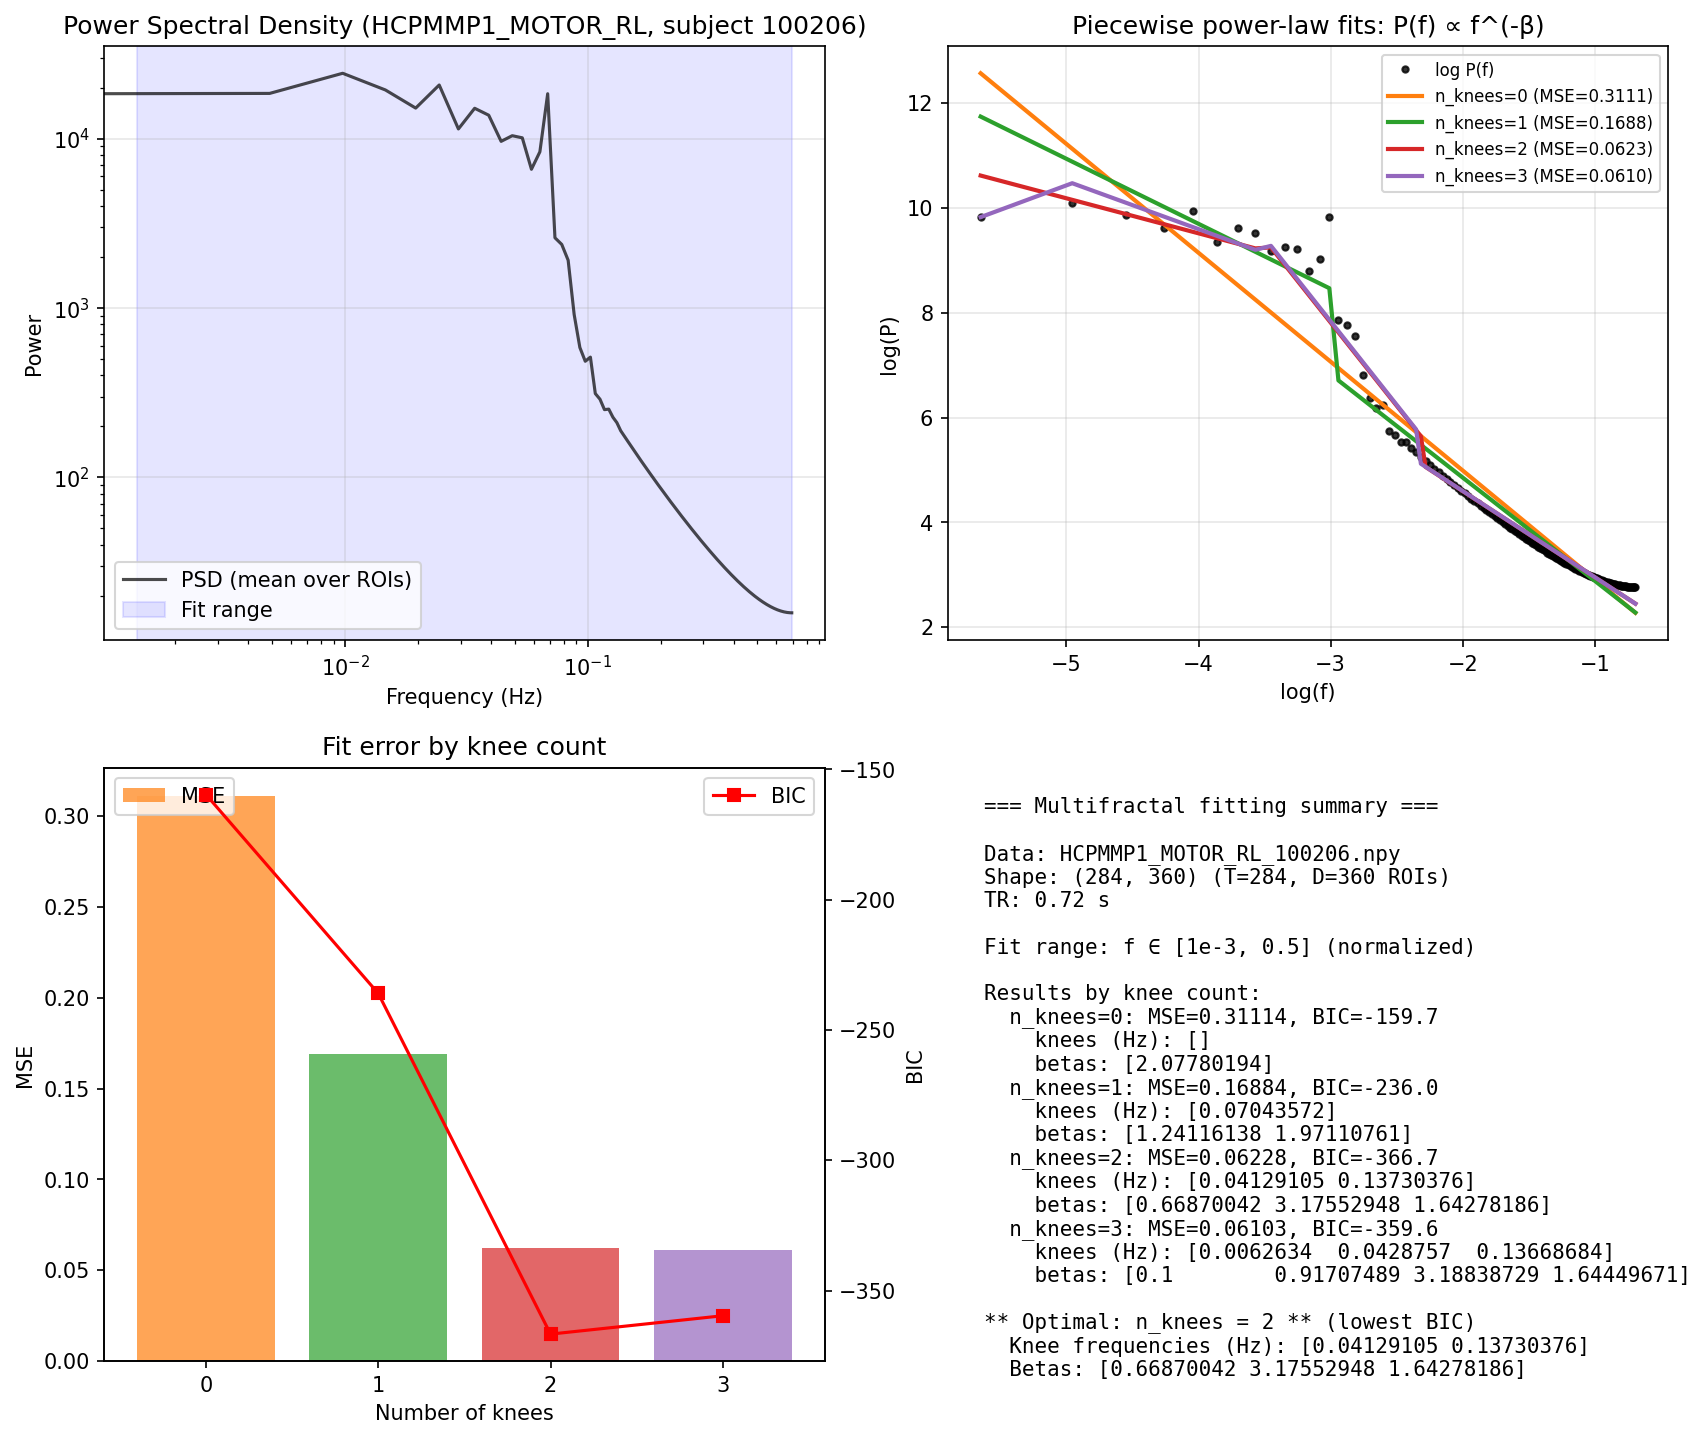
\includegraphics[width=\linewidth]{figures/motor_psd_multifractal.png}
\end{minipage}

\vspace{0.5em}

\begin{minipage}[b]{0.58\linewidth}
  \centering
  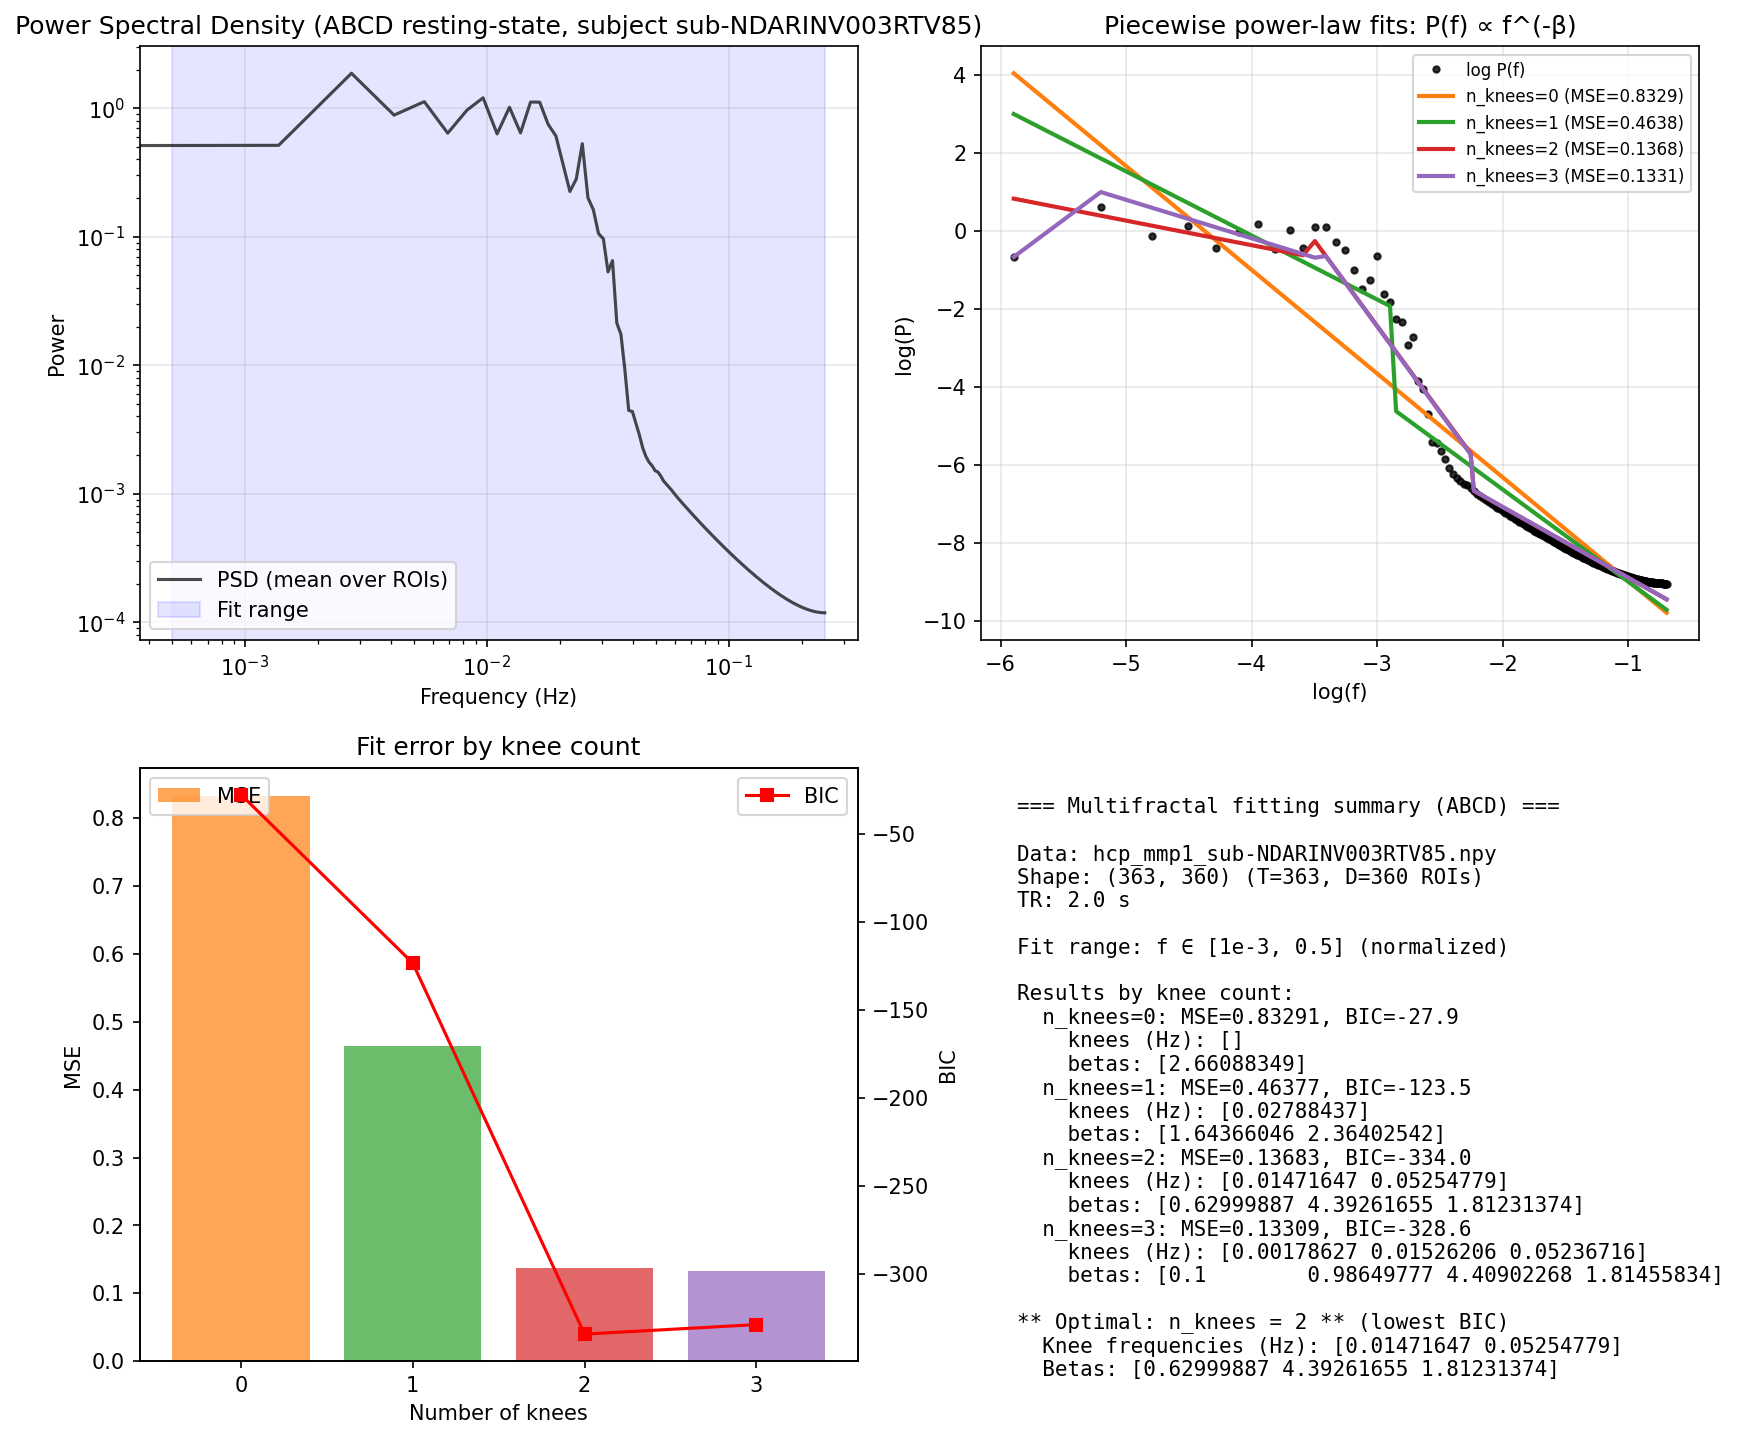
\includegraphics[width=\linewidth]{figures/abcd_psd_multifractal.png}
\end{minipage}

\caption{
\textbf{Piecewise power-law structure of empirical PSD across neural datasets.}
\textbf{(top left)} HCP resting-state fMRI (TR$=0.72$\,s, 360 cortical ROIs). The BOLD PSD exhibits distinct scaling regimes separated by knee frequencies $(f_1, f_2)$, consistent with the piecewise power-law model assumed by SpectralHyperNet.
\textbf{(top right)} HCP motor task fMRI (TR$=0.72$\,s, 360 ROIs). Task-evoked BOLD signals display a similar piecewise structure, indicating that the multi-scale power-law structure is not restricted to resting-state dynamics.
\textbf{(bottom)} ABCD resting-state fMRI. The piecewise power-law structure is preserved across a large developmental cohort with different acquisition parameters.
In each panel, the fitted piecewise model (dashed lines) accurately captures the observed spectral slope changes at the estimated knee frequencies, supporting the core spectral modeling assumption of PIMSM.
}
\label{fig:appx:psd_neural}
\end{figure}

\begin{figure}[htbp]
\centering
\begin{minipage}[b]{0.49\linewidth}
  \centering
  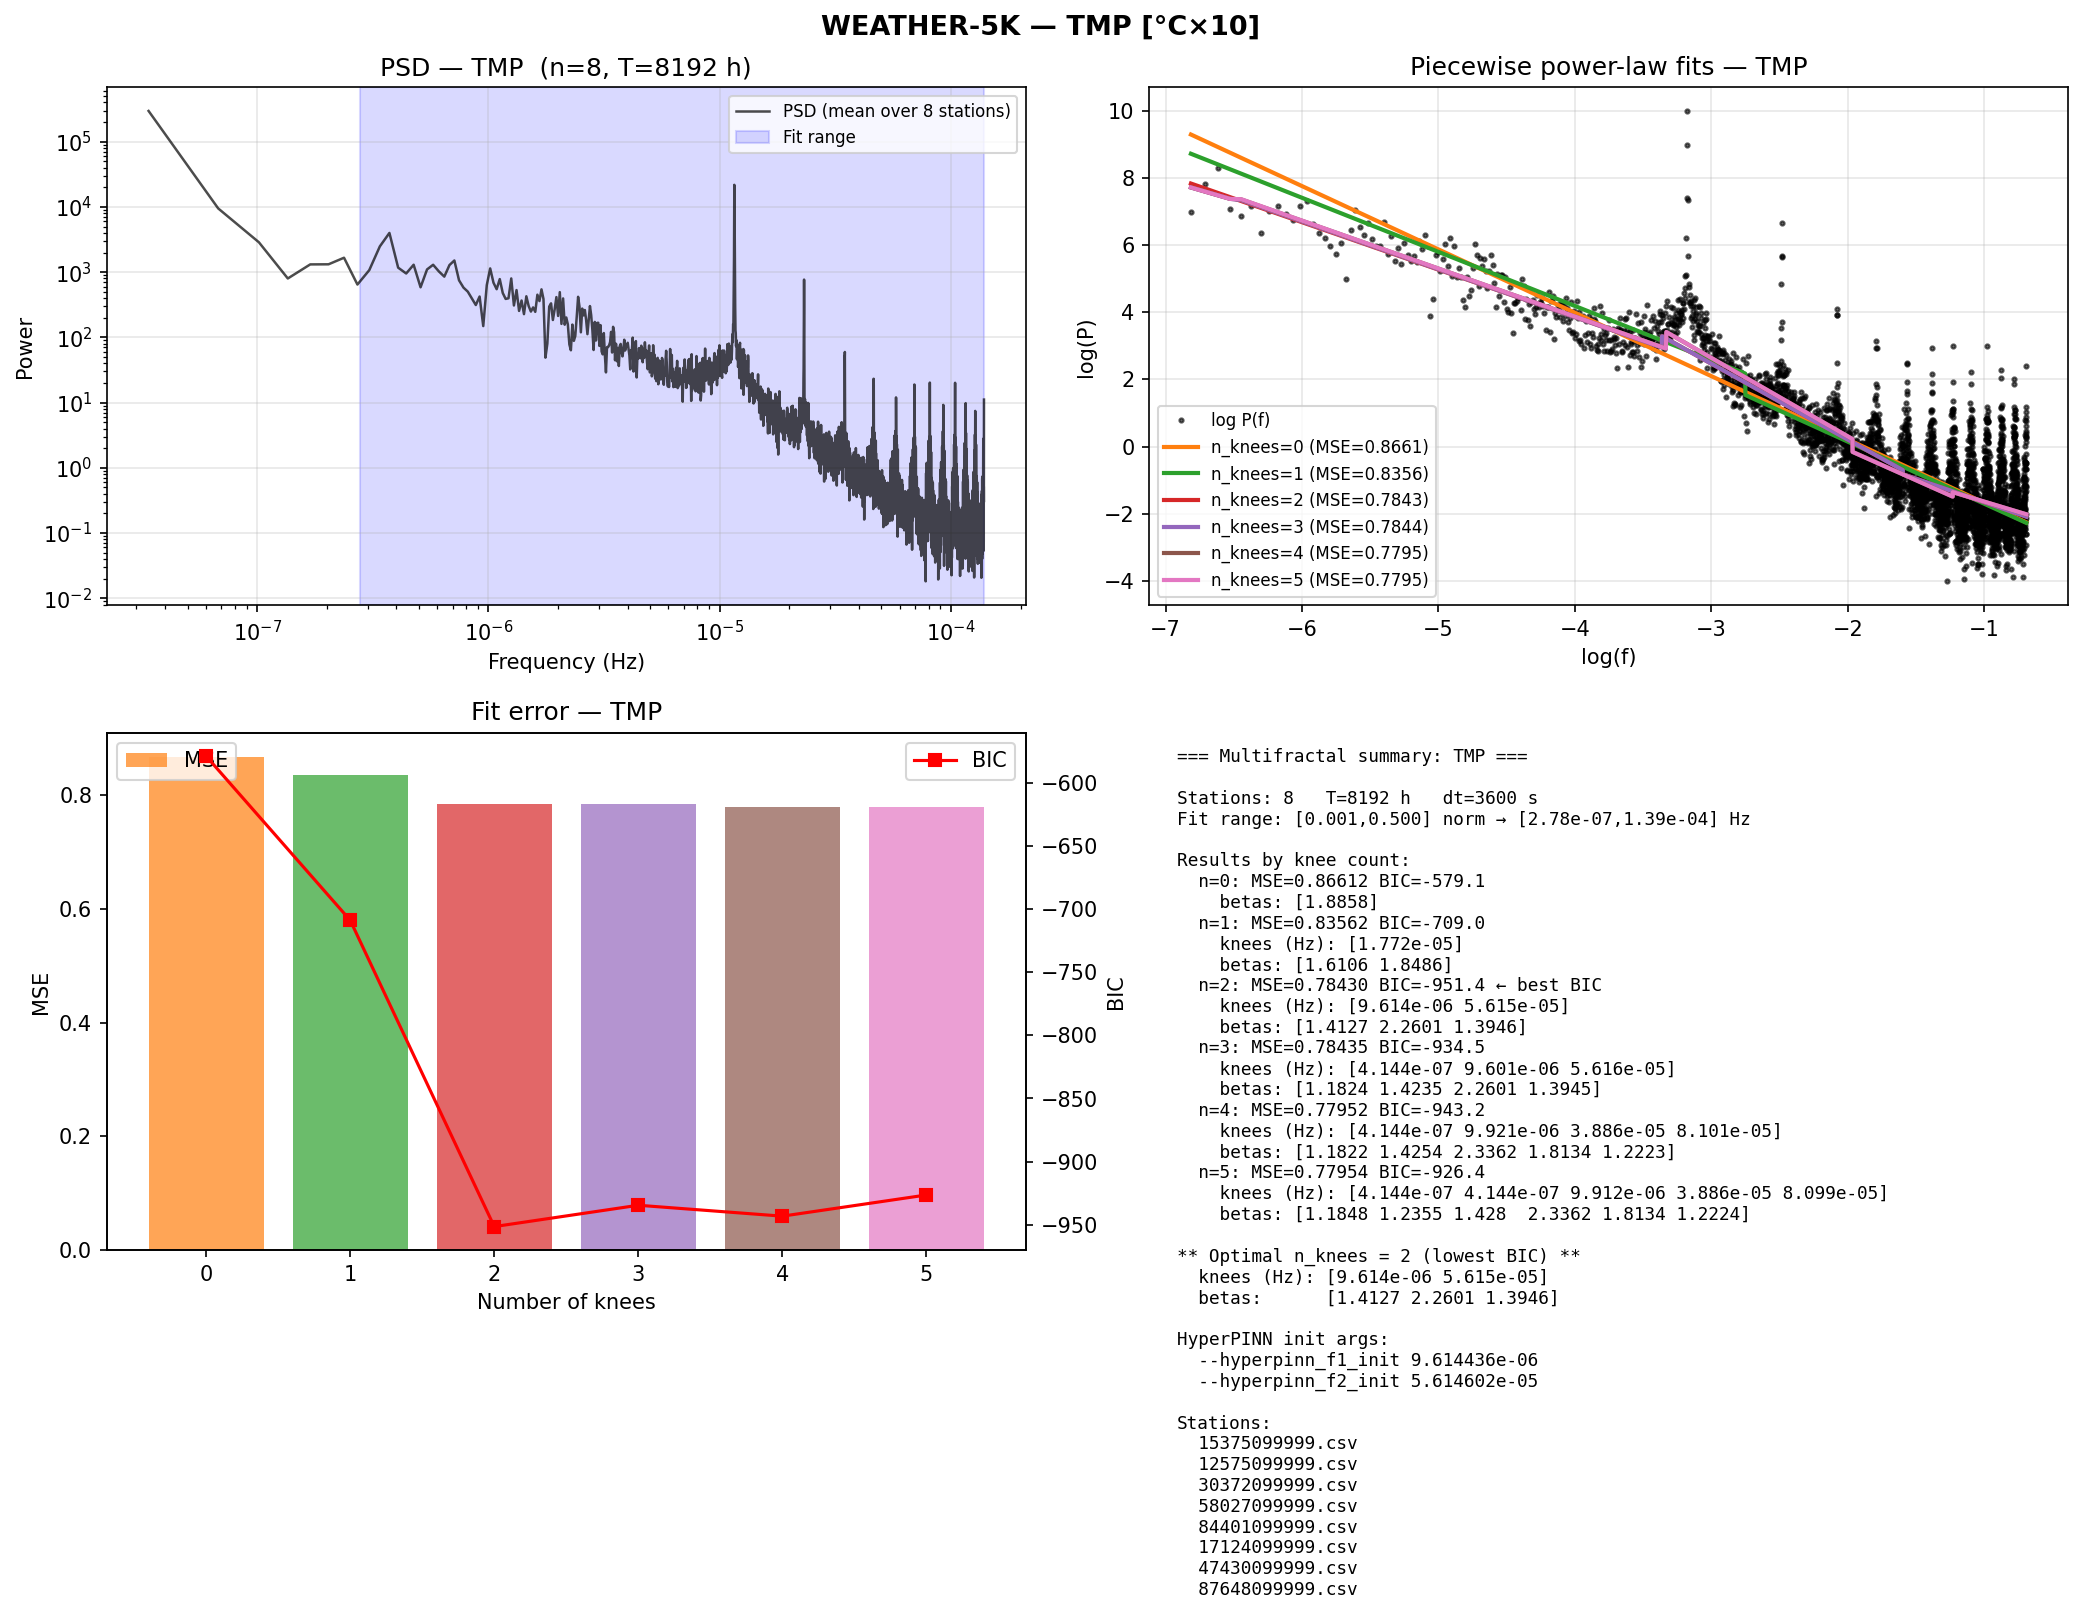
\includegraphics[width=\linewidth]{figures/weather5k_psd_tmp.png}
\end{minipage}
\hfill
\begin{minipage}[b]{0.49\linewidth}
  \centering
  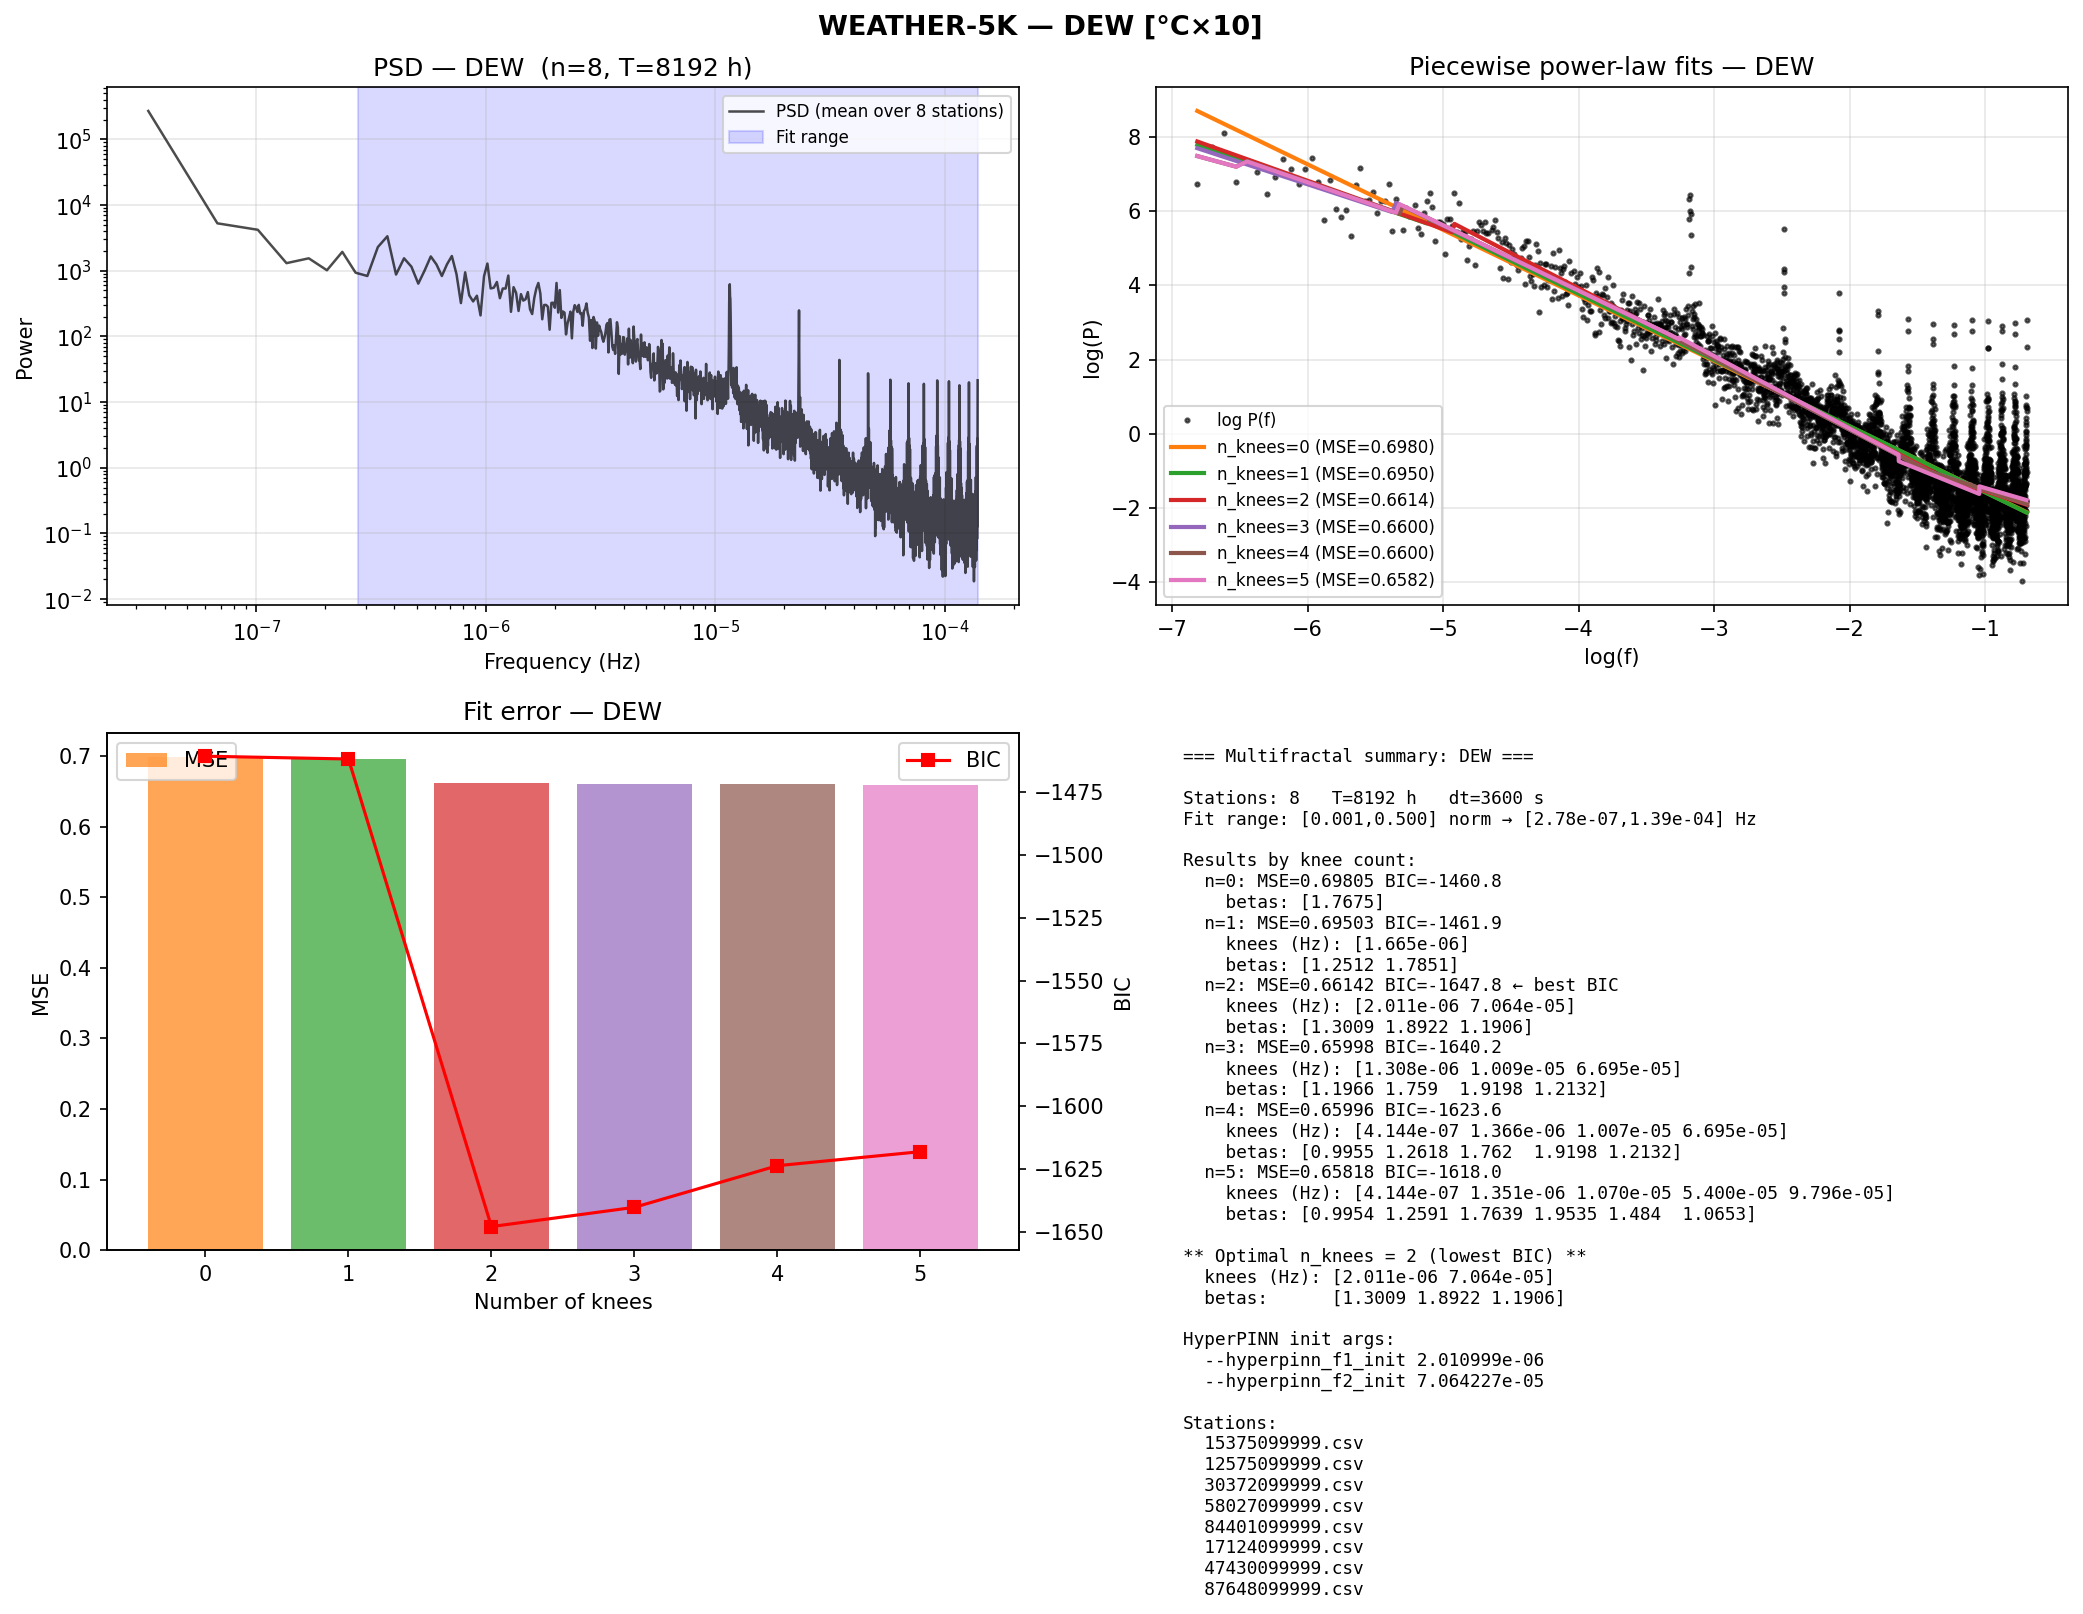
\includegraphics[width=\linewidth]{figures/weather5k_psd_dew.png}
\end{minipage}

\vspace{0.5em}

\begin{minipage}[b]{0.49\linewidth}
  \centering
  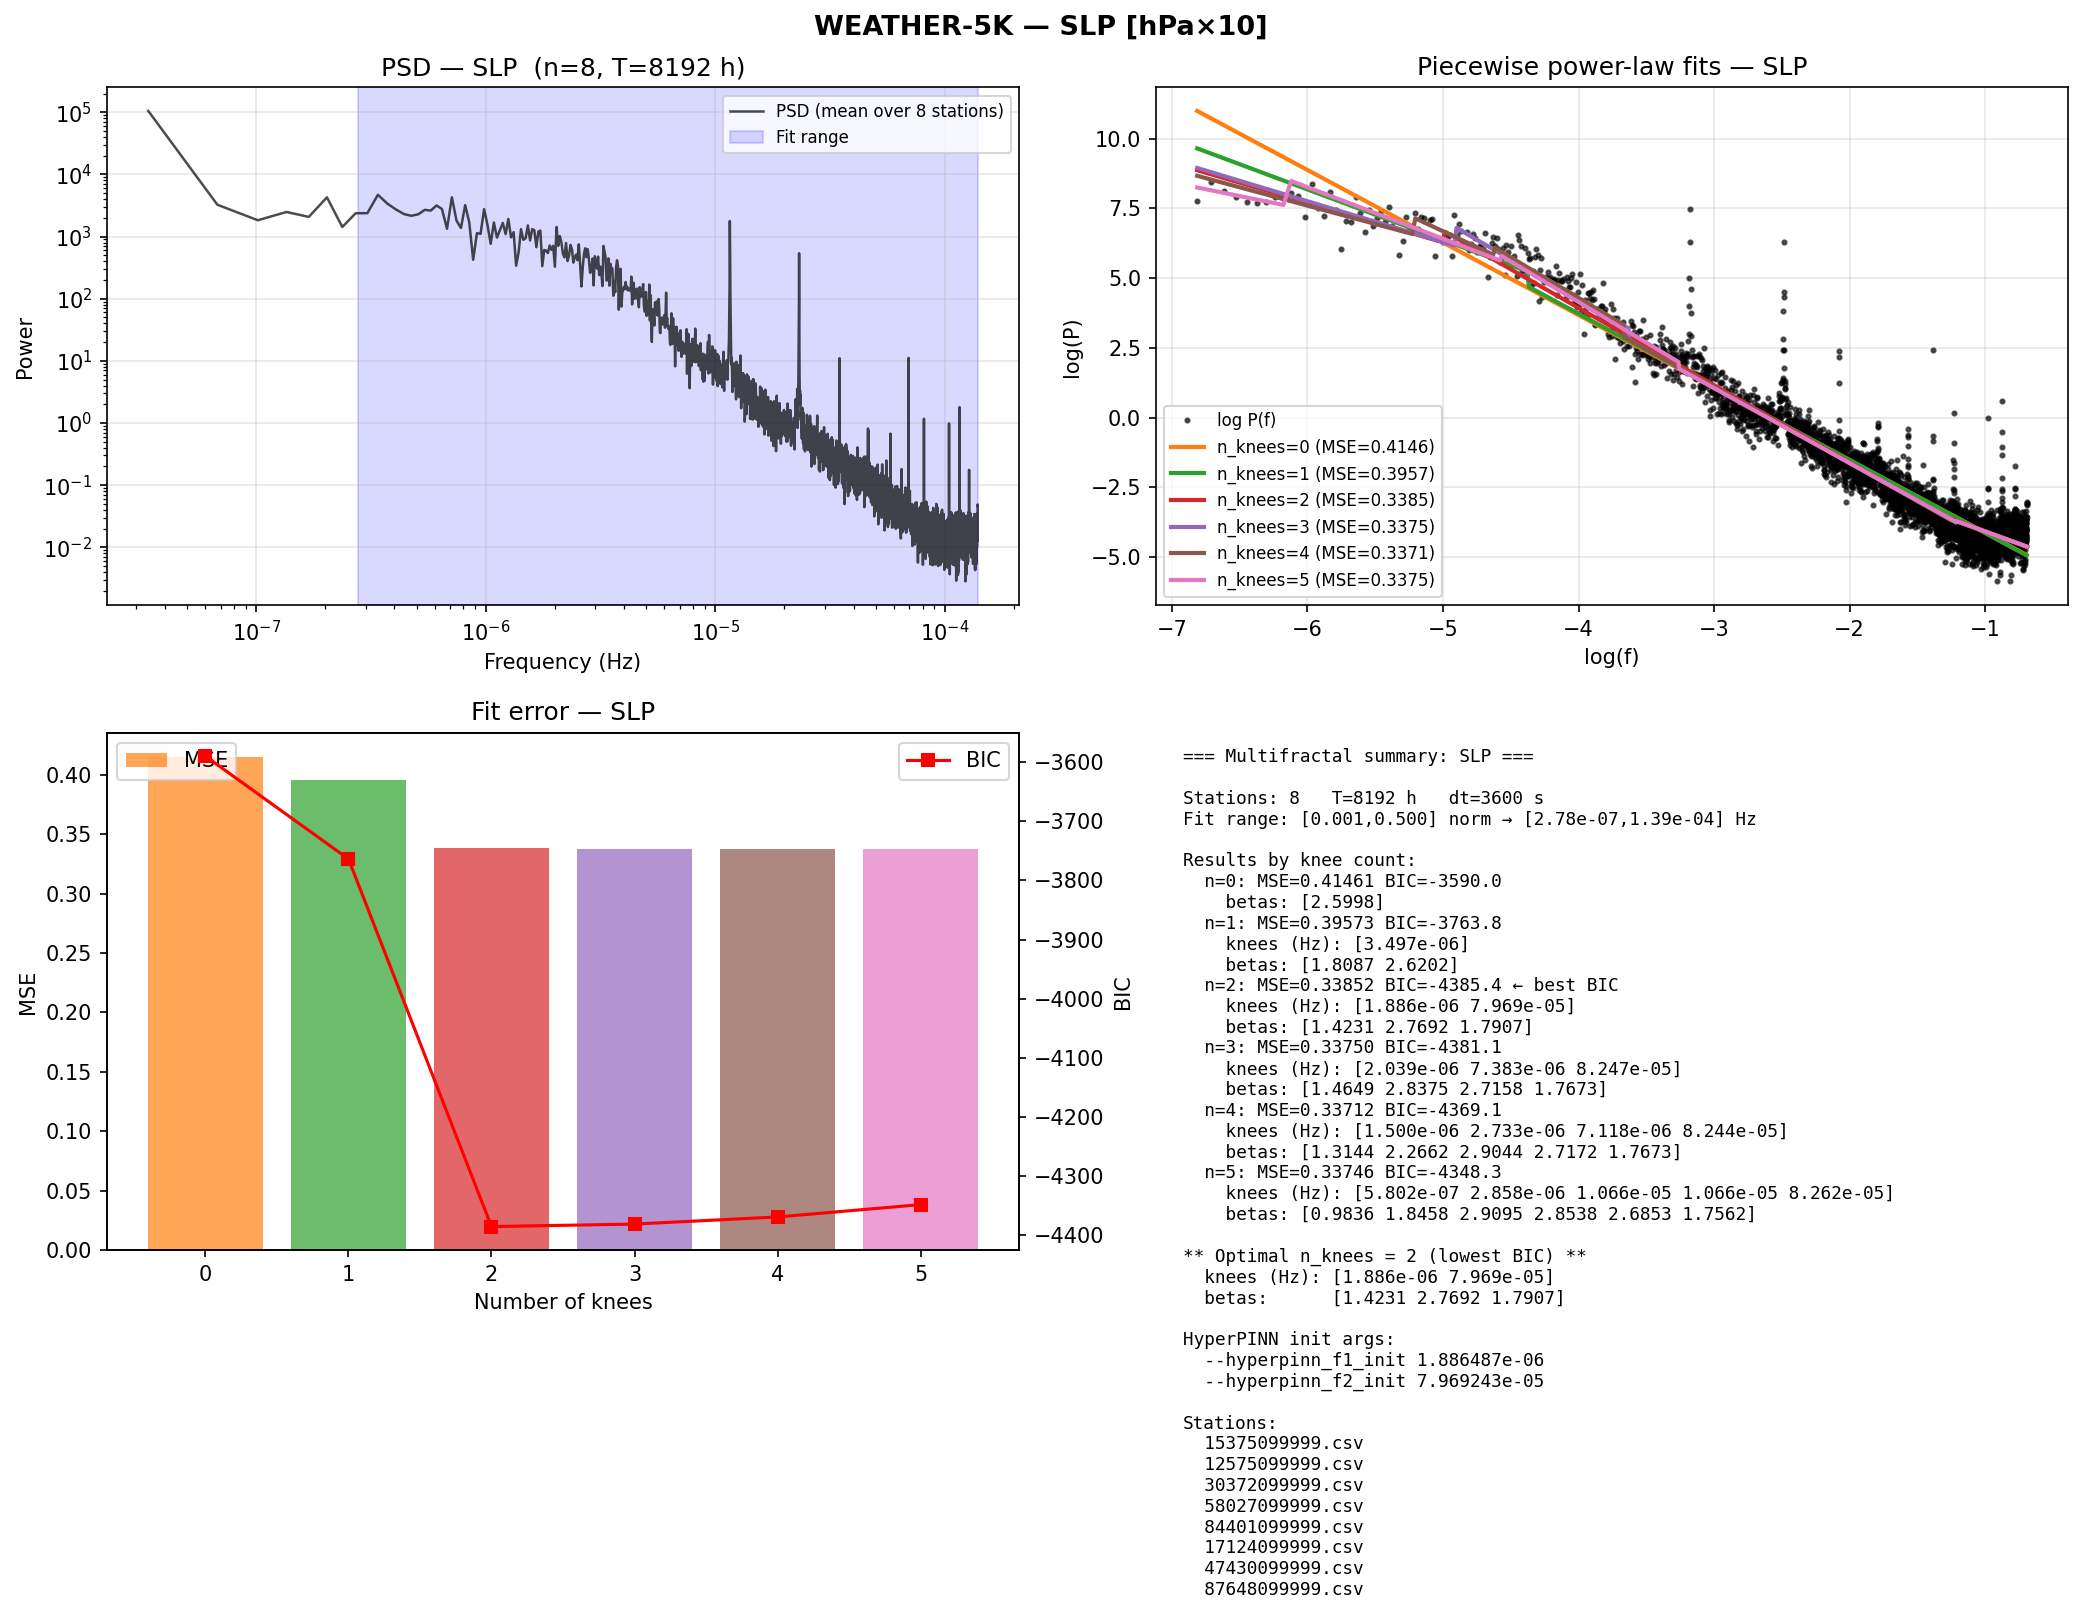
\includegraphics[width=\linewidth]{figures/weather5k_psd_slp.png}
\end{minipage}
\hfill
\begin{minipage}[b]{0.49\linewidth}
  \centering
  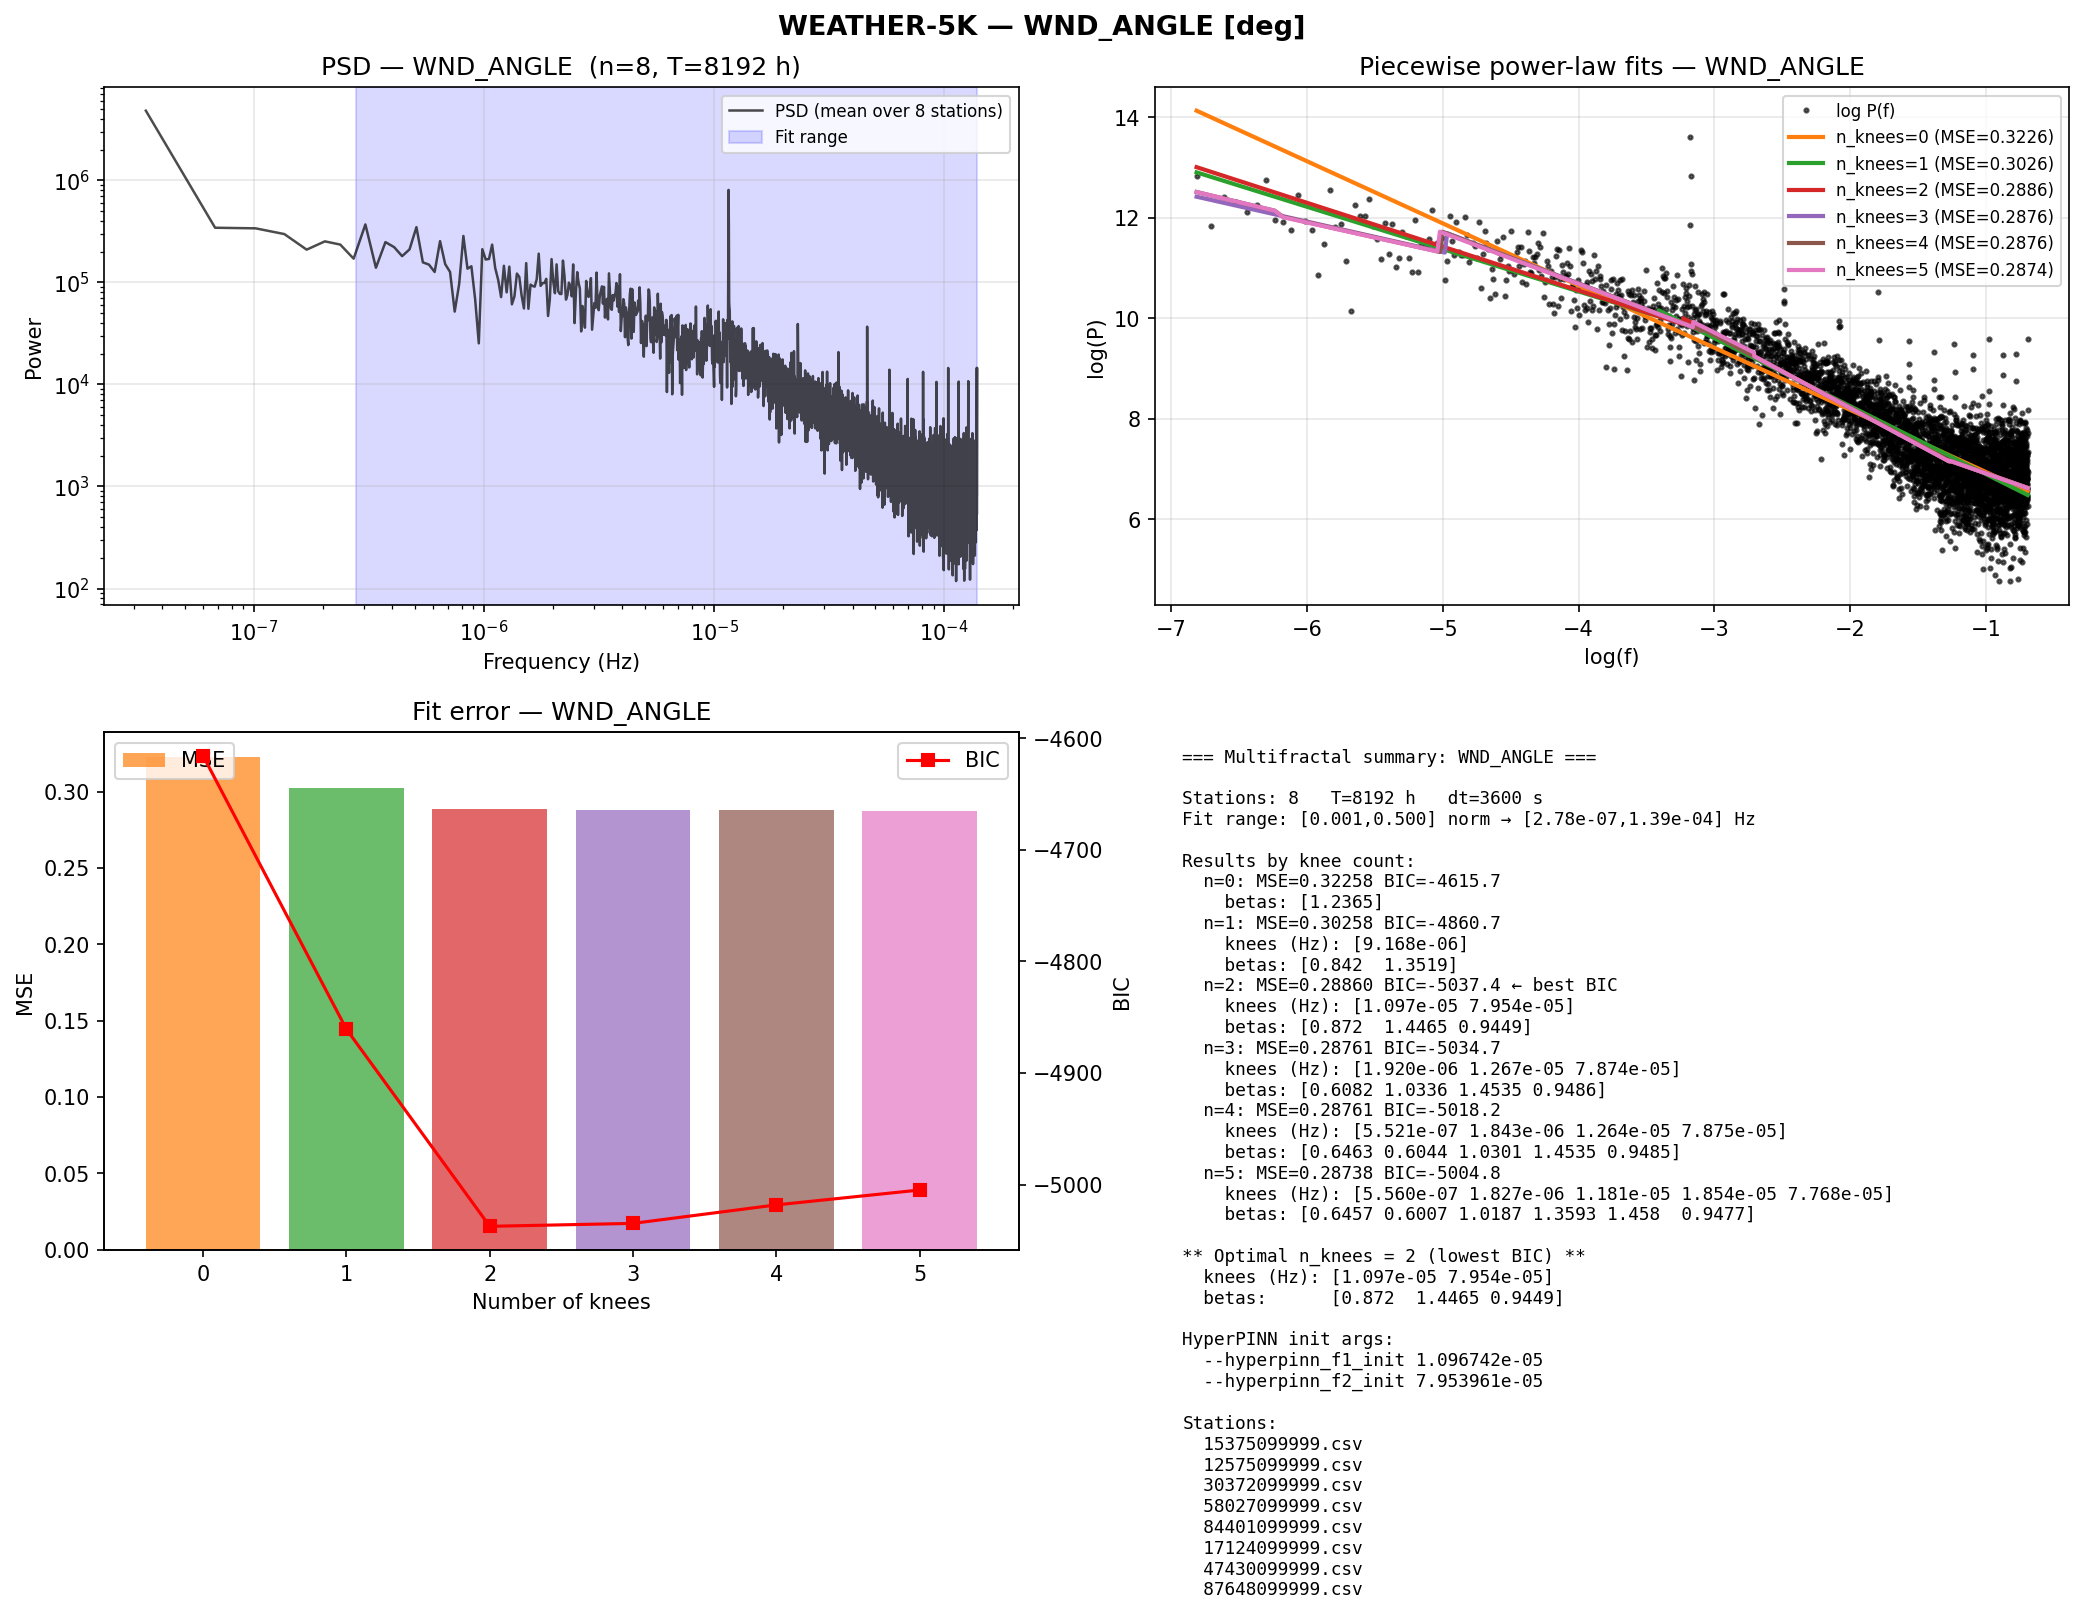
\includegraphics[width=\linewidth]{figures/weather5k_psd_wnd_angle.png}
\end{minipage}

\vspace{0.5em}

\begin{minipage}[b]{0.49\linewidth}
  \centering
  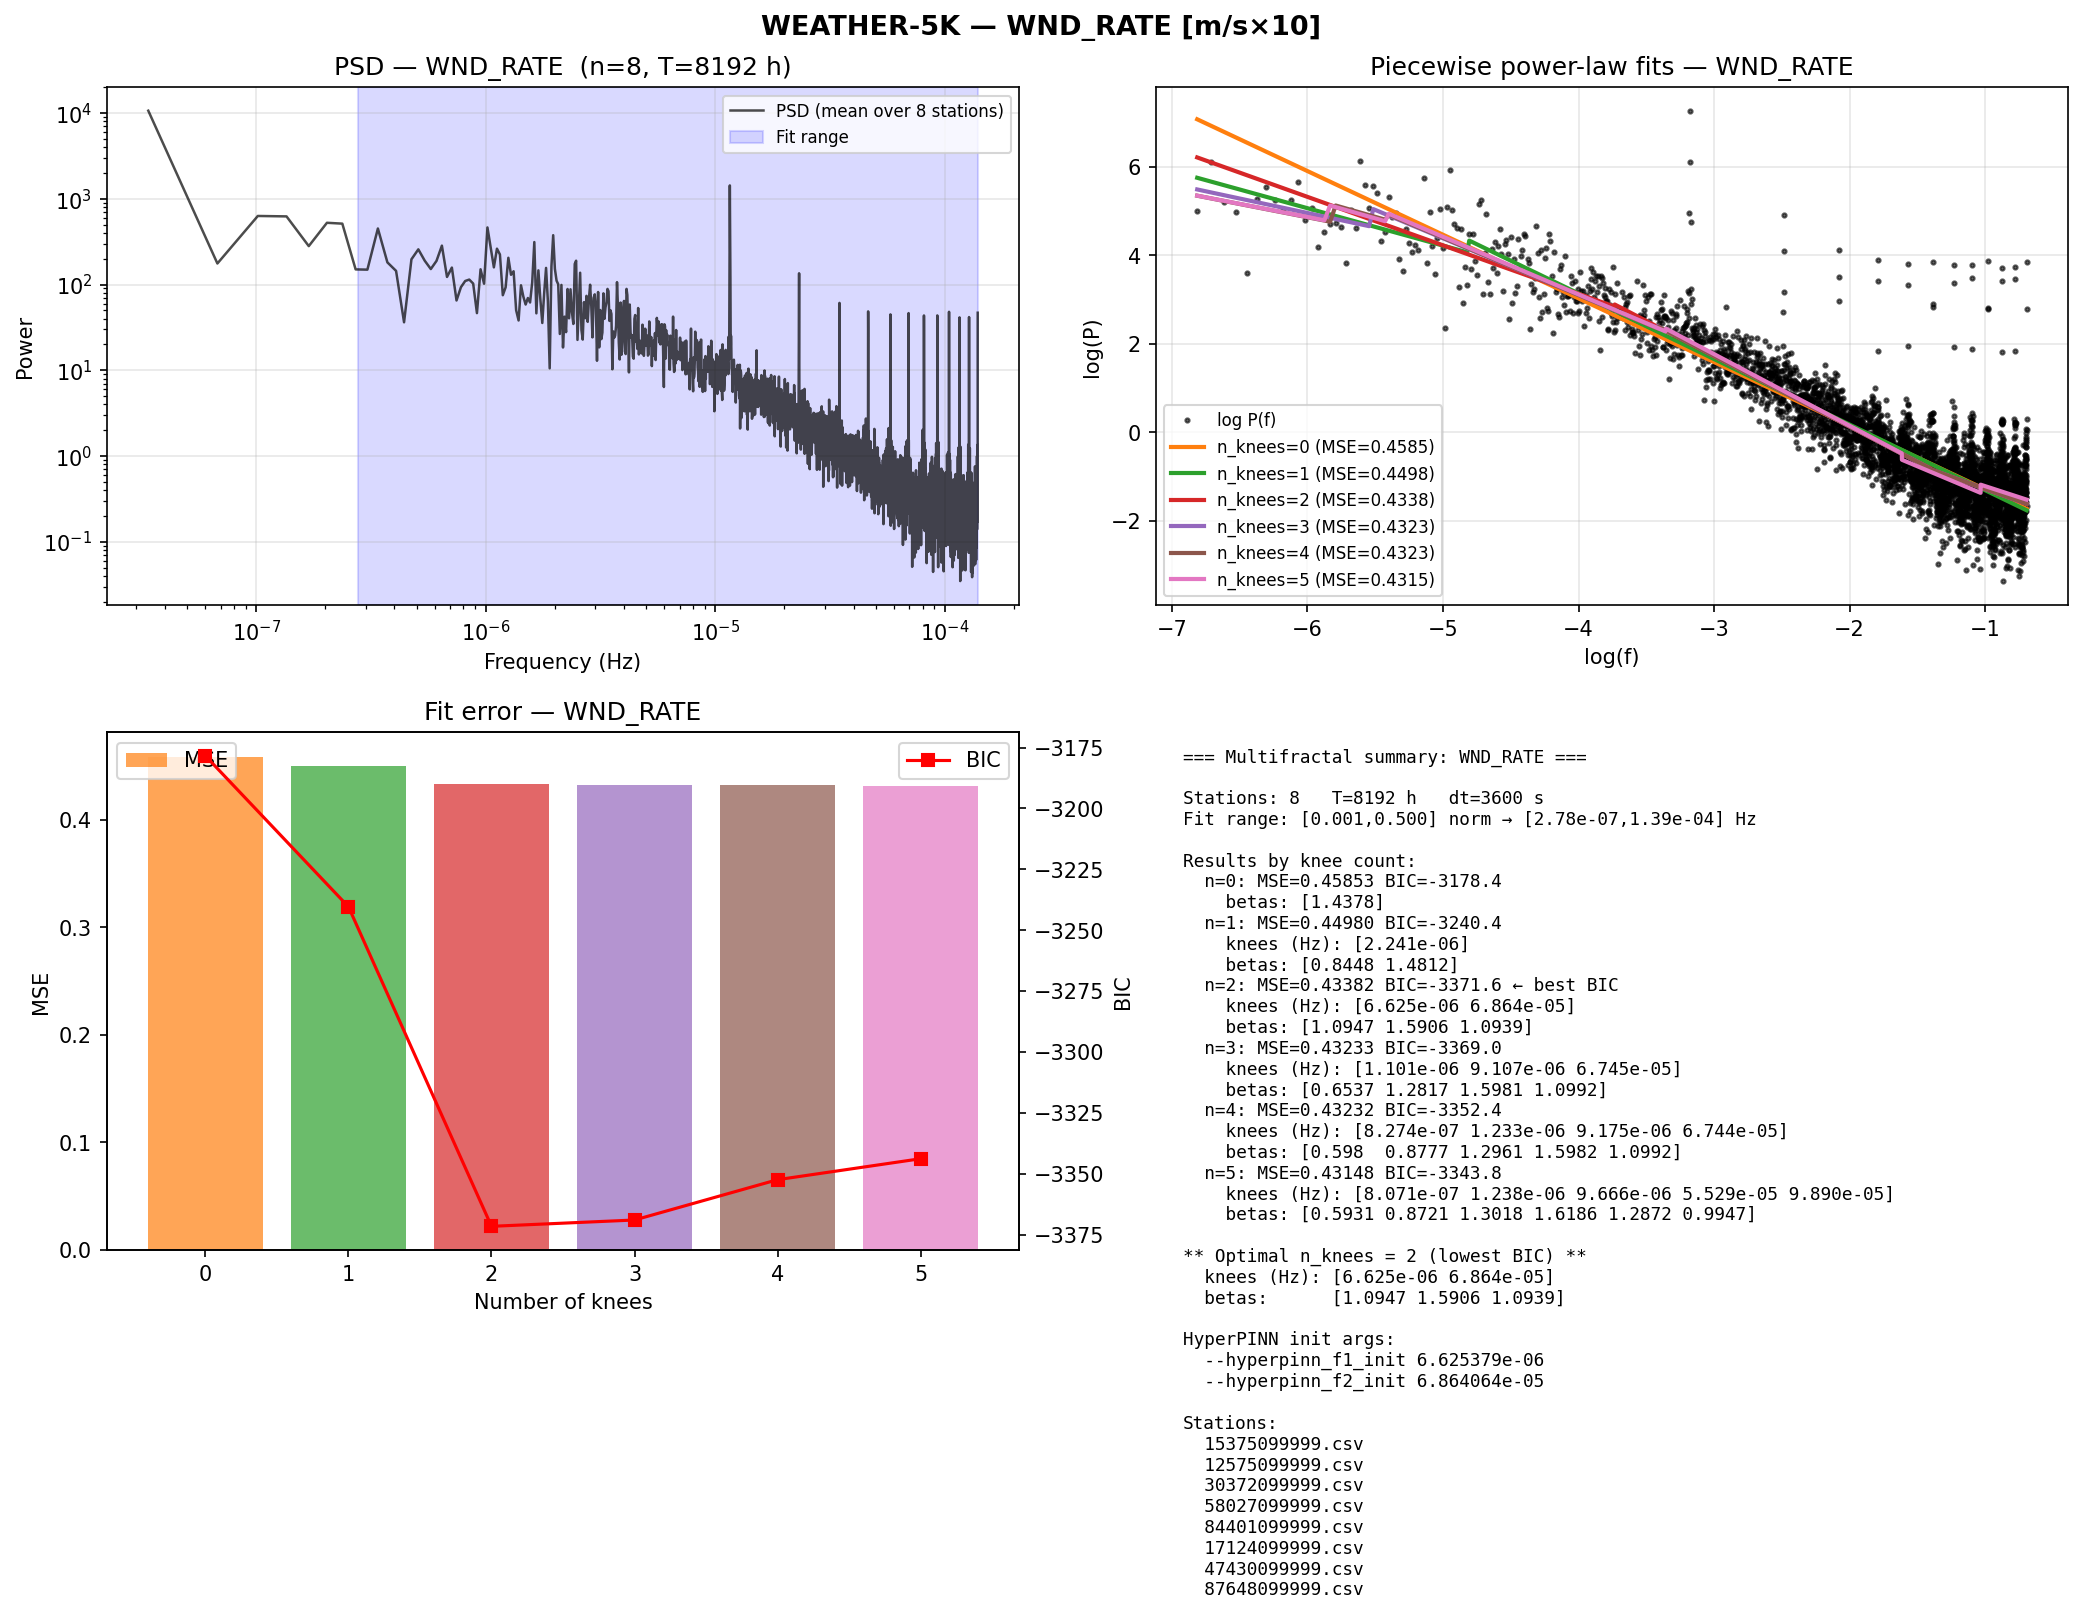
\includegraphics[width=\linewidth]{figures/weather5k_psd_wnd_rate.png}
\end{minipage}

\caption{
\textbf{Piecewise power-law structure of empirical PSD for Weather-5K (per variable).}
Weather-5K meteorological time series: temperature (tmp), dew point (dew), sea-level pressure (slp), wind angle (wnd\_angle), and wind rate (wnd\_rate).
Because PIMSM fits knee frequencies \emph{per variable}, each meteorological channel is analyzed independently rather than aggregated.
The piecewise power-law structure is consistent across all five variables, indicating that the spectral scaling assumption generalises beyond neural data.
In each panel, the fitted piecewise model (dashed lines) accurately captures the observed spectral slope changes at the estimated knee frequencies.
}
\label{fig:appx:psd_weather}
\end{figure}

We present empirical power spectral densities (PSDs) for fMRI cohorts and Weather-5K meteorological variables (Figures~\ref{fig:appx:psd_neural} and~\ref{fig:appx:psd_weather}).
Across all settings, the log-log PSD exhibits a piecewise linear structure with distinct scaling exponents $\beta_k$ separated by knee frequencies $(f_1, f_2)$, consistent with the piecewise power-law model in Eq.~\eqref{eq:piecewise_powerlaw}.
For the Weather-5K dataset, we fit the piecewise model \emph{independently per meteorological variable} (temperature, dew point, sea-level pressure, wind angle, wind rate), since each channel has its own characteristic spectral profile; PIMSM therefore infers a separate set of knee frequencies and scale-specific $\Delta_k$ for each variable.
This empirical regularity motivates the SpectralHyperNet-based scale inference at the heart of PIMSM: rather than imposing a single-exponent scaling law, we fit a configurable piecewise model (default $K=3$ in the main experiments) whose knee frequencies adaptively parameterize the scale-specific discretization parameters $\Delta_k$.

\section{Multi-scale Kernels Reduce Approximation Error to Power-Law Targets}
\label{sec:appx:kernel_approx}

We provide a theoretical result that formalizes the advantage of multi-scale exponential mixtures over single-scale models when approximating power-law decay kernels, which arise naturally from the piecewise power-law spectral structure of neural signals.

\paragraph{Setup.}
Consider the power-law decay kernel
\begin{equation}
g(t) = (1+t)^{-\alpha}, \qquad \alpha > 1,
\label{eq:powerlaw_kernel}
\end{equation}
which corresponds to long-memory temporal dependence.
This arises when the effective temporal kernel of a system integrates contributions from a continuum of timescales.
Let $\mathcal{G}_K$ denote the family of mixtures of $K$ exponentials:
\begin{equation}
\mathcal{G}_K \;=\; \left\{ \tilde{g}(t) = \sum_{k=1}^{K} a_k\, e^{-\lambda_k t} \;:\; a_k \ge 0,\; \sum_{k=1}^K a_k = 1,\; \lambda_k > 0 \right\}.
\label{eq:G_K}
\end{equation}
An SSM whose effective dynamics are dominated by one discretization scale can be viewed as a $K=1$ approximation, while PIMSM with $K$ explicit scales corresponds to $\mathcal{G}_K$.

\begin{proposition}[Multi-scale approximation of power-law kernels]
\label{prop:kernel_approx}
Let $g(t) = (1+t)^{-\alpha}$ with $\alpha > 1$.
There exists a constant $C_\alpha > 0$ depending only on $\alpha$ such that:
\begin{equation}
\inf_{\tilde{g} \in \mathcal{G}_K} \|g - \tilde{g}\|_{L^1[0,\infty)} \;\leq\; C_\alpha \cdot K^{-(\alpha-1)}.
\label{eq:multi_scale_approx_bound}
\end{equation}
In contrast, for $K=1$:
\begin{equation}
\inf_{\tilde{g} \in \mathcal{G}_1} \|g - \tilde{g}\|_{L^1[0,\infty)} \;=\; \Omega(1),
\label{eq:single_scale_floor}
\end{equation}
i.e., the approximation error is bounded away from zero by a positive constant independent of the choice of $\lambda_1$.
\end{proposition}

\paragraph{Proof sketch.}
The key insight is the Stieltjes (Laplace) representation of $g$:
\begin{equation}
g(t) = (1+t)^{-\alpha} = \frac{1}{\Gamma(\alpha)} \int_0^\infty \lambda^{\alpha-1} e^{-\lambda} e^{-\lambda t}\, d\lambda \;\propto\; \int_0^\infty e^{-\lambda t}\, \mu(\lambda)\, d\lambda,
\label{eq:stieltjes}
\end{equation}
where the mixing measure is $\mu(\lambda) \propto \lambda^{\alpha-2}$ (up to normalization) for $\lambda \in (0, \infty)$.
Thus $g$ is a continuous mixture of exponentials, and the best $K$-exponential approximation corresponds to a $K$-point quadrature rule for the measure $\mu$.

\emph{Upper bound (Eq.~\eqref{eq:multi_scale_approx_bound}).}
Choose $\lambda_1 < \lambda_2 < \cdots < \lambda_K$ as the nodes of a $K$-point Gauss--Jacobi quadrature rule adapted to $\mu$, with corresponding weights $a_k$.
By standard quadrature error theory, the $L^2$ error in approximating $\int_0^\infty e^{-\lambda t} \mu(\lambda)\, d\lambda$ decays as $O(K^{-2(\alpha-1)})$ for smooth $\mu$ with polynomial growth $\mu(\lambda) \propto \lambda^{\alpha-2}$.
Applying Cauchy--Schwarz to convert from $L^2$ to $L^1[0,\infty)$ yields Eq.~\eqref{eq:multi_scale_approx_bound}.

\emph{Lower bound (Eq.~\eqref{eq:single_scale_floor}).}
A single exponential $a_1 e^{-\lambda_1 t}$ cannot reproduce the algebraic tail of $(1+t)^{-\alpha}$: for any $\lambda_1 > 0$, the $L^1$ difference $\int_0^\infty |(1+t)^{-\alpha} - a_1 e^{-\lambda_1 t}|\, dt$ remains bounded away from zero because exponentials decay faster than any power law.
This follows from the fact that $e^{-\lambda t} = o((1+t)^{-\alpha})$ as $t \to \infty$ for all $\lambda > 0$ and $\alpha > 1$, giving an $\Omega(1)$ tail discrepancy regardless of the choice of $a_1, \lambda_1$.

\paragraph{Implication for PIMSM.}
Proposition~\ref{prop:kernel_approx} establishes that the approximation error of $\mathcal{G}_K$ to a power-law kernel decreases at rate $K^{-(\alpha-1)}$, while a single exponential ($K=1$) incurs a nonvanishing floor error.
For $\alpha = 2$ (canonical $1/f$ scaling), $K = 3$ reduces the upper bound by a factor of $3^{(\alpha-1)} = 3$ relative to $K=1$.
Combined with Lemma~\ref{lem:kernel_mismatch} (Section~\ref{sec:theory:kernelbound}), this suggests why a 3-scale SSM can reduce representation error relative to a one-scale approximation when the target kernel is well modeled by a power-law decay.

\paragraph{Physics-informed quadrature.}
Proposition~\ref{prop:kernel_approx} shows that \emph{any} $K$-point quadrature achieves the $K^{-(\alpha-1)}$ rate.
PIMSM's SpectralHyperNet provides a structured quadrature: the knee frequencies $(f_1, f_2)$ inferred from the empirical PSD determine the quadrature nodes $\{\lambda_k\}$ in a data-adaptive manner.
Compared to randomly initialized or freely learnable scale parameters (which may cluster in suboptimal regions of the $\lambda$ axis), the physics-informed initialization places the quadrature nodes near the spectral knees of the target distribution, yielding a better-conditioned approximation.
This provides a theoretical mechanism underlying the empirical advantage of SpectralHyperNet-derived $\Delta$ parameters over random or learnable alternatives in the TR-shift experiments (Appendix~\ref{sec:appx:hcp_tr_shift}).

\section{Delta Mapping Ablation: Mixing Weight and Normalization Mode}
\label{sec:appx:delta_ablation}

The per-band frequency-to-delta mapping combines global band position $p_k$ and within-band normalized frequency $t_k$ via $m_k = p_k(1-w) + w\,t_k$. To assess sensitivity to this design choice, we ablate (i) the mixing weight $w \in \{0, 0.3, 0.5, 1.0\}$ and (ii) normalization mode (global vs.\ per-band). At $w=0$, $m_k = p_k$ (band position only); at $w=1$, $m_k = t_k$ (within-band variation only); the default $w=0.3$ balances both. Global normalization maps $f_{c,k}$ directly onto $[\Delta_{\min}, \Delta_{\max}]$ without per-band boundaries. These ablations are designed to verify that the core principle---higher $f \to$ larger $\Delta$---drives the benefit, rather than the specific mixing formula.

\section{Dataset and Preprocessing Details}
\label{sec:appx:data}

\paragraph{HCP-1200 motor task fMRI.}
Time series were extracted from 360 cortical regions (HCPMMP1 atlas~\citep{glasser2016multi}), yielding inputs $\mathbf{x}_{1:T}\in\mathbb{R}^{T\times360}$ (TR$=0.72$\,s).
Event-related segments for five motor conditions (LH, RH, LF, RF, T) were extracted with a maximum block length of 17 TRs; each ROI time series was z-score normalized per run.
\textbf{Temporal-context shift:} SpectralHyperNet receives the full trial sequence for spectral calibration, while the SSM backbone input is truncated to the first 3 or 2 TRs. This tests early-window decoding with full-sequence spectral scale estimates, not a change in scanner TR or sampling rate.
\textbf{Low-resource:} labeled fraction varied in $\{1\%, 5\%, 10\%, 100\%\}$; validation and test sets unchanged.

\paragraph{HCP resting-state fMRI (brain-state shift).}
Models trained on resting-state fMRI (truncated to 284 TRs) for sex classification, then evaluated on HCP motor-task fMRI (284 TRs, same subjects, disjoint test split) without adaptation.

\paragraph{Weather-5K.}
Large-scale meteorological benchmark~\citep{han2024far} spanning 5,672 global weather stations.
We use hourly station records with five raw meteorological variables: temperature (TMP), dew point (DEW), wind angle, wind rate, and sea-level pressure (SLP). Wind angle is circular, so it is represented as sine and cosine components, giving six model channels: TMP, DEW, wind-sin, wind-cos, wind rate, and SLP. Missing rows are dropped before window construction.

For matched experiments we use a 100-station geo-stratified subset. Stations are sampled from geographic clusters built from latitude, longitude, elevation, and station quality metadata, with a target cluster size of eight stations. The spatial OOD split then partitions stations, not windows: stations are clustered on unit-sphere geographic coordinates, clusters are ranked by geographic isolation, and the most isolated cluster(s) are assigned to the held-out test set. We use this station-disjoint split as the primary Weather-5K evaluation because chronological holdouts share station identity between train and test, while spatial holdout evaluates generalization to unseen station domains. In the current runs, 90\% of stations are used for training/validation and 10\% are held out for spatial OOD testing. Within the train-station set, $1/9$ of windows are used for validation, yielding an approximate 8:1:1 train/validation/test station-window budget while keeping test stations disjoint from training.

Normalization statistics for z-scoring are computed from training inputs only. For train stations, per-station mean and standard deviation are estimated from training windows; held-out spatial OOD stations fall back to the global training statistics because their station-specific statistics are unavailable during training. RevIN is then applied on top of this dataset-level normalization during model training and evaluation, and predictions are mapped back to variable units before reporting MAE.

\section{Formal Problem Setup}
\label{sec:appx:problem_setup}

We observe a multivariate time series $x_{1:T} \in \mathbb{R}^{d}$.
A temporal encoder $\Phi_{\theta}$ maps $x_{1:T}$ to latent states $h_{1:T} = \Phi_{\theta}(x_{1:T})$, $h_t \in \mathbb{R}^m$.
An aggregation $z = \rho(h_{1:T})$ feeds a prediction head $\hat{y} = g_{\psi}(z)$.
Given labeled source data $\mathcal{D}_{e}$, training minimizes
\begin{equation}
\min_{\theta,\psi}\;\mathbb{E}_{(x,y)\sim \mathcal{D}_{e}}\!\left[\ell\!\left(g_{\psi}(\rho(\Phi_{\theta}(x))),\,y\right)\right].
\end{equation}
Representation drift under shift $e \to e'$ is defined in Eq.~\eqref{eq:drift_def} of the main text.
The physics-informed spectral assumption is: the power spectral density of $x$ admits a piecewise scaling form $S_x(f) \approx c_k f^{-\beta_k}$, $f \in [f_{k-1}, f_k]$, $k=1,\dots,K$, motivating scale-specific discretization parameters $\Delta^{(k)}$ tied to the knee frequencies $(f_1,\dots,f_{K-1})$.

\section{Theory Proofs}
\label{sec:appx:proofs}

\subsection{Proof of Lemma~\ref{lem:kernel_mismatch} (Kernel Mismatch Bound)}

\begin{proof}
For any $t$,
\[
|h(t)-\tilde h(t)|
=
\left|\int_{0}^{\infty} (g(\tau)-\tilde g(\tau))\, x(t-\tau)\, d\tau\right|
\le
\int_{0}^{\infty} |g(\tau)-\tilde g(\tau)|\, |x(t-\tau)|\, d\tau
\le
M \int_{0}^{\infty} |g(\tau)-\tilde g(\tau)|\, d\tau.
\]
Taking the supremum over $t$ gives Eq.~\eqref{eq:kernel_mismatch_bound}.
\end{proof}

\subsection{Proposition: Readout Sensitivity to Representation Drift}

\begin{proposition}[Readout sensitivity]
\label{prop:readout_sensitivity}
For any $w$ and representations $(h,h')$,
\begin{equation}
|\hat y' - \hat y| = |w^\top(h'-h)| \le \|w\|_2\,\|h'-h\|_2.
\end{equation}
\end{proposition}

\begin{proof}
Cauchy--Schwarz inequality applied directly.
\end{proof}

\bibliography{references}

%%%%%%%%%%%%%%%%%%%%%%%%%%%%%%%%%%%%%%%%%%%%%%%%%%%%%%%%%%%%

\newpage
\input{checklist.tex}


\end{document}
